\section{Renormalization Group Procedure for Effective Particles (RGPEP)}
\label{sec:rgpep}

Divergences appering in Hamiltonian quantum field theories come from far off-diagonal matrix elements. 
These matrix elements arise from interactions between particles of vastly different energy scales. \cite{}
The similarity renormalization group \cite{} applies a unitary transformation $U(\lambda)$ to a matrix $H$, where $\lambda$ is interpretted as an energy scale. 
In general, the unitary transformation defined by $H(\lambda) = U(\lambda)HU^\dagger(\lambda)$ ``lowers the energy scale'' in which interactions can happen. 
This is realized by a continuous transformation to $H$, parameterized by $\lambda$ that makes the original matrix increasingly diagonal. 
In doing this, the spectrum is preserved, but the matrix elements that lead to divergences are removed.

In practice, the parameter $\lambda$ is exchanged for $t$, where $t \sim 1/\lambda$. 
This is because it is easier to scale $t$ from $0 \rightarrow \infty$, than to scale $\lambda$ from $\infty \rightarrow 0$ (higher energy scales to lower).
Determining the rate of change in $t$ of the Hamiltonian $H$ leads us to determining a form of $U(t)$:

\begin{equation}
    \label{eq:rgpep-ut}
    \frac{dH(t)}{dt} = \left[\frac{dU(t)}{dt}U^\dagger(t), H(t) \right]
\end{equation}

The first term in the commutator, $\frac{dU(t)}{dt}U^\dagger(t)$ is called the \textit{generator} $\left(\mathcal{G}(t) \right)$, which is what is chosen, rather than $U(t)$ itself.
In general, any generator can be chosen (in the same way that any $U$ could be); however, the generator that ``pushes'' the matrix towards the diagonal, and is commonly used in literature is $\mathcal{G}(t) \equiv \left[H_0, H(t) \right]$
Thus, the RGPEP equation is given as 

\begin{equation}
    \label{eq:rgpep}
    \frac{dH(t)}{dt} = \left[\mathcal{G}(t), H(t) \right]
\end{equation}

This equation holds true for any matrix; however, in quantum field theories, the Hamiltonians are written as integrals of creation and annihilation operators. 
Given a set of Fock states, one could construct a matrix, and solve equation \ref{eq:rgpep}; however, the renormalization group procedure for effective particles (RGPEP) \cite{} offers an alternative approach.

RGPEP is based on the similarity renormalization group, but rather than calculating commutators of matrices, it is done by commutators of creation and annihilation operators. 
In general, the RGPEP equation cannot be solved exactly, so it must be solved order-by-order in $g$.
This is accomplished by expanding $H$ as 

\begin{equation}
    \label{eq:H-expansion}
    H(t) = H_0(t) + gH^{(1)}(t) + g^2 H^{(2)}(t) + \mathcal{O}(g^3).
\end{equation}

Asserting this form of $H(t)$ in equation \ref{eq:rgpep}, we obtain

\begin{equation}
    g\dot{H}^{(1)}(t) + g^2\dot{H}^{(2)}(t) + \dots = \left[\left[H_0, H_0 + gH^{(1)}(t) + g^2H^{(2)}(t) + \dots\right], H_0 + gH^{(1)}(t) + g^2H^{(2)}(t) + \dots\right].
\end{equation}

Thus, 

\begin{align}
    \label{eq:rgpep-order-by-order}
    &\mathcal{O}(g^0): \dot{H}_0 = 0\\ \nonumber
    &\mathcal{O}(g^1): g\dot{H}^{(1)}(t) = \left[\left[H_0, gH^{(1)}(t)\right], H_0\right] \\\nonumber
    &\mathcal{O}(g^2): g^2\dot{H}^{(2)}(t) = \left[\left[H_0, g^2H^{(2)}(t)\right], H_0\right] + \left[\left[H_0, gH^{(1)}(t)\right],gH^{(1)}(t)\right] \\ \nonumber
    &\vdots
\end{align}

The first equation is trivial, with solution $H_0(t) = H_0$. 
Higher order solutions, however, are not as simple to solve.
The following sections explain procedures to solve these higher-order equations.

\subsection{$\mathcal{O}(g)$ Solution}
\label{sec:first-order}
At first order in $g$, the RGPEP equation is 

\begin{equation}
    \label{eq:first-order}
    \frac{dH^{(1)}(t)}{dt} = \left[\left[H_0, H^{(1)}(t) \right], H_0 \right].
\end{equation}

We can see that the inner commutator in equation \ref{eq:first-order} is the same form as the generator, but at first order only. 
Thus, we define $\mathcal{G}^{(1)}(t) = \left[H_0,  H^{(1)}(t)\right]$.

The first order part of $H$ is given in equation \ref{eq:yukawa-hamiltonian}.
To determine how $H^{(1)}$ evolves in $t$, we must add explicit \textit{t}-dependence to the coefficients of $H^{(1)}$.
This is done by substituting the coefficients in front of each product of creation and annihilation operators with arbitrary coefficients that depend not only on momenta, but also $t$. 
For example, the coefficient in front of $b_i^\dagger b_j a_k$ changes from $$4\pi \delta\left(p_i^+ - p_j^+ - p_k^+ \right)\bar u(p_i) u(p_j) \rightarrow c_{ijk}(t)$$  
The rest of the coefficients can similarly be exchanged for a paramterized version, where it is important to modify the coefficient in a way that it is clear which term it modifies:

\begin{align}\nonumber
    4\pi \delta\left(p_i^+ + p_k^+ - p_j^+ \right)\bar{u}(p_i) u(p_j) &\rightarrow c^*_{ikj}(t)\\ \nonumber
    4\pi \delta\left(p_i^+ - p_j^+ - p_k^+ \right)\bar{v}(p_j) v(p_i) &\rightarrow \bar{c}_{ijk}(t) \\ \nonumber
    4\pi \delta\left(p_i^+ + p_k^+ - p_j^+ \right)\bar{v}(p_j) v(p_i) &\rightarrow \bar c^*_{ikj}(t)\\ \nonumber
    4\pi \delta\left(p_i^+ + p_j^+ - p_k^+ \right)\bar{u}(p_i) v(p_j) &\rightarrow \tilde c_{ijk}(t)\\ \nonumber
    4\pi \delta\left( p_k^+ - p_i^+ - p_j^+ \right)\bar{v}(p_j) u(p_i) &\rightarrow \tilde c^*_{kij}(t)\\ \nonumber
\end{align}

The Hamiltonian now assumes a simpler form:

\begin{align}
    \label{eq:H-first-order-c-coeffs}
    H^{(1)}(t) = g\int_i \int_j \int_k &\left(c_{ijk}(t)b_i^\dagger b_j a_k + c_{ikj}^*(t) b_i^\dagger b_j a_k^\dagger + \bar c_{ijk}(t) d_i^\dagger d_j a_k \right. \\ \nonumber
    & \left. \bar c^*_{ikj}(t) d^\dagger_i d_j a_k^\dagger + \tilde c_{ijk}(t)b_i^\dagger d_j^\dagger a_k + \tilde c^*_{kij}(t) b_i d_j a_k^\dagger \right).
\end{align}

where
\begin{equation}
    \int_i \rightarrow \int_0^\infty \frac{dp_i^\dagger}{4\pi p_i^+}
\end{equation}

We similarly modify the free part of the Hamiltonian as

\begin{equation}
    H_0 = \int_n B_n b_n^\dagger b_n + \int_n D_n d_n^\dagger d_n + \int_n A_n a_n^\dagger a_n.
\end{equation}

The inner commutator in equation \ref{eq:first-order} modifies each term in the Hamiltonian by the coefficients in the free part $H_0$.
For example, the first term in equation \ref{eq:H-first-order-c-coeffs} corresponds to fermion $+$ boson in, fermion out. 
The term thus gets modified by $\left(B_i - D_j - A_k\right)$.
Continuing this with every term arrives at:

\begin{align}
    \label{eq:first-order-inner-commutator}
    \left[H_0, H^{(1)}(t) \right] &= g\int_i \int_j \int_k \left(\left(B_i - B_j - A_k \right)c_{ijk}(t)b_i^\dagger b_j a_k + \left(B_i + A_k - B_j\right)c_{ikj}^*(t) b_i^\dagger b_j a_k^\dagger + \left(D_i - D_j - A_k \right)\bar c_{ijk}(t) d_i^\dagger d_j a_k \right. \\ \nonumber
    & \left. \left(D_i + A_k - D_j\right)\bar c^*_{ikj}(t) d^\dagger_i d_j a_k^\dagger + \left(B_i + D_j - A_k\right)\tilde c_{ijk}(t)b_i^\dagger d_j^\dagger a_k + \left(A_k - B_i - D_j \right)\tilde c^*_{kij}(t) b_i d_j a_k^\dagger \right).
\end{align}

To get the full right hand side of equation \ref{eq:first-order}, we do another commutator of equation \ref{eq:first-order-inner-commutator} with $H_0$, which gives another factor of the modificiations of the form $B_i + D_j - A_k$, with a negative sign ($H_0$ is on the right of the commutator now). 

\begin{align}
    \label{eq:RHS-first-order}
    \left[\left[H_0, H^{(1)}(t) \right], H_0\right] = g\int_i \int_j \int_k &\left(-\left(B_i - B_j - A_k \right)^2c_{ijk}(t)b_i^\dagger b_j a_k - \left(B_i + A_k - B_j\right)^2c_{ikj}^*(t) b_i^\dagger b_j a_k^\dagger \right. \\ \nonumber
    &\left. - \left(D_i - D_j - A_k \right)^2\bar c_{ijk}(t) d_i^\dagger d_j a_k -\left(D_i + A_k - D_j\right)^2\bar c^*_{ikj}(t) d^\dagger_i d_j a_k^\dagger\right. \\ \nonumber
    & \left.  - \left(B_i + D_j - A_k\right)^2\tilde c_{ijk}(t)b_i^\dagger d_j^\dagger a_k - \left(A_k - B_i - D_j \right)^2\tilde c^*_{kij}(t) b_i d_j a_k^\dagger \right).
\end{align}

If we differentiate equation \ref{eq:H-first-order-c-coeffs}, the coefficients in $t$ now become derivatives in $t$.
Term by term, we can equate the derivatives on the left hand side of \ref{eq:first-order} with the corresponding term from equation \ref{eq:RHS-first-order}.
For example, 

\begin{equation}
    \frac{d}{dt}c_{ijk}(t) = -\left(B_i - B_j - A_k \right)^2 c_{ijk}(t)
\end{equation}

which has solution 

\begin{equation}
    c_{ijk}(t) = c_{ijk}(0)e^{-\left(B_i - B_j - A_k \right)^2t}
\end{equation}
where $c_{ijk}(0)$ comes from the initial Hamiltonian we wrote down: $c_{ijk}(0) = 4\pi \delta\left(p_i^+ - p_j^+ - p_k^+ \right)\bar u(p_i) u(p_j)$.
Thus, the full first order solution is given as:
 
\begin{align}
    &H^{(1)}(t) = \int_0^\infty\int_0^\infty\int_0^\infty \frac{dp_i^+dp_j^+dp_k^+}{\left(4\pi \right)^3 p_i^+ p_j^+ p_k^+}\left(4\pi \delta\left(p_i^+ - p_j^+ - p_k^+ \right) \bar u(p_i) u(p_j) e^{-\left(\frac{m_F^2}{p_i^+} - \frac{m_F^2}{p_j^+} - \frac{m_B^2}{p_k^+} \right)^2t} b_i^\dagger b_j a_k \right.\\ \nonumber
    &\left. +4\pi \delta\left(p_i^+ + p_k^+- p_j^+  \right) \bar u(p_i) u(p_j) e^{-\left(\frac{m_F^2}{p_i^+} + \frac{m_B^2}{p_k^+} - \frac{m_F^2}{p_j^+}  \right)^2t} b_i^\dagger b_j a_k^\dagger + 4\pi \delta\left(p_i^+ - p_j^+ - p_k^+ \right) \bar v(p_j) v(p_i) e^{-\left(\frac{m_{\bar F}^2}{p_i^+} - \frac{m_{\bar F}^2}{p_j^+} - \frac{m_B^2}{p_k^+} \right)^2t} d_i^\dagger d_j a_k \right. \\ \nonumber
    &\left.  +4\pi \delta\left(p_i^+ + p_k^+ - p_j^+ \right) \bar v(p_j) v(p_i) e^{-\left(\frac{m_{\bar F}^2}{p_i^+} + \frac{m_B^2}{p_k^+} - \frac{m_{\bar F}^2}{p_j^+}  \right)^2t} d_i^\dagger d_j a_k^\dagger + 4\pi \delta\left(p_i^+ + p_j^+ - p_k^+ \right) \bar u(p_i) v(p_j) e^{-\left(\frac{m_F^2}{p_i^+} + \frac{m_{\bar F}^2}{p_j^+} - \frac{m_B^2}{p_k^+} \right)^2t} b_i^\dagger d_j^\dagger a_k \right. \\ \nonumber
    & \left.  +4\pi \delta\left(p_i^+ + p_j^+ - p_k^+ \right) \bar v(p_j) u(p_i) e^{-\left(\frac{m_B^2}{p_k^+} - \frac{m_F^2}{p_i^+} - \frac{m_{\bar F}^2}{p_j^+}  \right)^2t}b_i d_j a_k^\dagger\right)\\ \nonumber
\end{align}

It is important to note that the exponentials in $t$ are referred to as \textit{form factors}.

\subsection{$\mathcal{O}(g^2)$ Solution}
\label{sec:second-order}
At second order in $g$, the RGPEP equation is more involved:

\begin{equation}
    \label{eq:rgpep-second-order}
g^2\dot{H}^{(2)}(t) = \left[\left[H_0, g^2H^{(2)}(t)\right], H_0\right] + \left[\left[H_0, gH^{(1)}(t)\right],gH^{(1)}(t)\right]
\end{equation}

At first glance at equation \ref{eq:yukawa-hamiltonian}, it appears as if only the instantaneous terms make up $H^{(2)}(t)$. 
However, it is important to add to $H^{(2)}(t)$ higher order terms arising from combining two $\mathcal{O}(g)$ interactions. 
Computing the second commutator in equation \ref{eq:rgpep-second-order} reveals the $\mathcal{O}(g^2)$ interaction terms. 
This commutator is written as $$\left[\mathcal{G}^{(1)}(t), H^{(1)}(t) \right].$$
Using Wick's theorem, we can simplify this commutator \footnote{For example, to compute $\left[b_n^\dagger b_n, b_x^\dagger b_y a_z \right] = b_n^\dagger b_nb_x^\dagger b_y a_z - b_x^\dagger b_y a_zb_n^\dagger b_n$, we first normal order both terms and induce Dirac deltas: $b_n^\dagger b_nb_x^\dagger b_y a_z - b_x^\dagger b_y a_zb_n^\dagger b_n = b_n^\dagger \left(\delta_{nx} - b_x^\dagger b_n \right)b_y a_z - b_x^\dagger \left(\delta_{ny} - b_n^\dagger b_y \right)b_n a_z = \delta_{nx}b_n^\dagger b_y a_z - \delta_{ny}b_x^\dagger b_n a_z$. This is the difference between normal ordered contractions in the last line of equation \ref{eq:commutator-to-contractions}}: 

\begin{align}
    \label{eq:commutator-to-contractions}
    \left[\mathcal{G}^{(1)}(t), H^{(1)}(t) \right] &= \mathcal{G}^{(1)}(t)H^{(1)}(t) - H^{(1)}(t)\mathcal{G}^{(1)}(t)\\ \nonumber
    &= :\mathcal{G}^{(1)}(t)H^{(1)}(t): + :C\left(\mathcal{G}^{(1)}(t)H^{(1)}(t)\right): - :H^{(1)}(t)\mathcal{G}^{(1)}(t): - :C\left(H^{(1)}(t)\mathcal{G}^{(1)}(t) \right):\\ \nonumber
    &=:C\left(\mathcal{G}^{(1)}(t)H^{(1)}(t)\right): - :C\left(H^{(1)}(t) \mathcal{G}^{(1)}(t)\right):.\\ \nonumber
\end{align} 

Here, it is assumed that $:\mathcal{G}^{(1)}(t)H^{(1)}(t): = H^{(1)}(t)\mathcal{G}^{(1)}(t): $ since the number of fermions (antifermions) always come in pairs in any quantum field theory.

We can continue simplifying equation \ref{eq:commutator-to-contractions}:

\begin{align}
    \label{eq:full-simplification-of-GH-comm}
    \left[\mathcal{G}^{(1)}(t), H^{(1)}(t) \right] &= :C\left(\mathcal{G}^{(1)}(t)H^{(1)}(t)\right): - :C\left(H^{(1)}(t) \mathcal{G}^{(1)}(t)\right):\\ \nonumber
    &= \sum_{D_1, D_2} \left(:C\left(\mathcal{G}_{D_1}^{(1)}(t)H_{D_2}^{(1)}(t)\right): - :C\left(H^{(1)}_{D_1}(t) \mathcal{G}^{(1)}_{D_2}(t)\right) \right) \\ \nonumber
    &= \sum_{contractions} \left(\mathcal{P}_A + \mathcal{P}_B -2\mathcal{P}_C  \right)V_1(0) V_2(0)T_{contraction}
\end{align}

To understand the final form of equation \ref{eq:full-simplification-of-GH-comm}, we note $D_i \in \{\text{Yukawa interactions} \}$. 
Thus, we calculate contractions of every pair of interaction terms in $H^{(1)}(t)$ (since interaction terms in $\mathcal{G}^{(1)}(t)$ are the same, up to some coefficient modifications).
After writing down every possible contraction, we now have $\mathcal{O}(g^2)$ interaction diagrams, labeled by $T_{contraction}$, which describes the ladder operator structure of the term. 
Instead of meticulously keeping track of indices, the last line in equation \ref{eq:full-simplification-of-GH-comm} allows you to take a given contraction from two interactions, and gives the modification to the coefficient needed to write out the commutator in equation \ref{eq:full-simplification-of-GH-comm}.
An example is given in figures \ref{fig:D1D2} and \ref{fig:contraction}.

\begin{figure}
    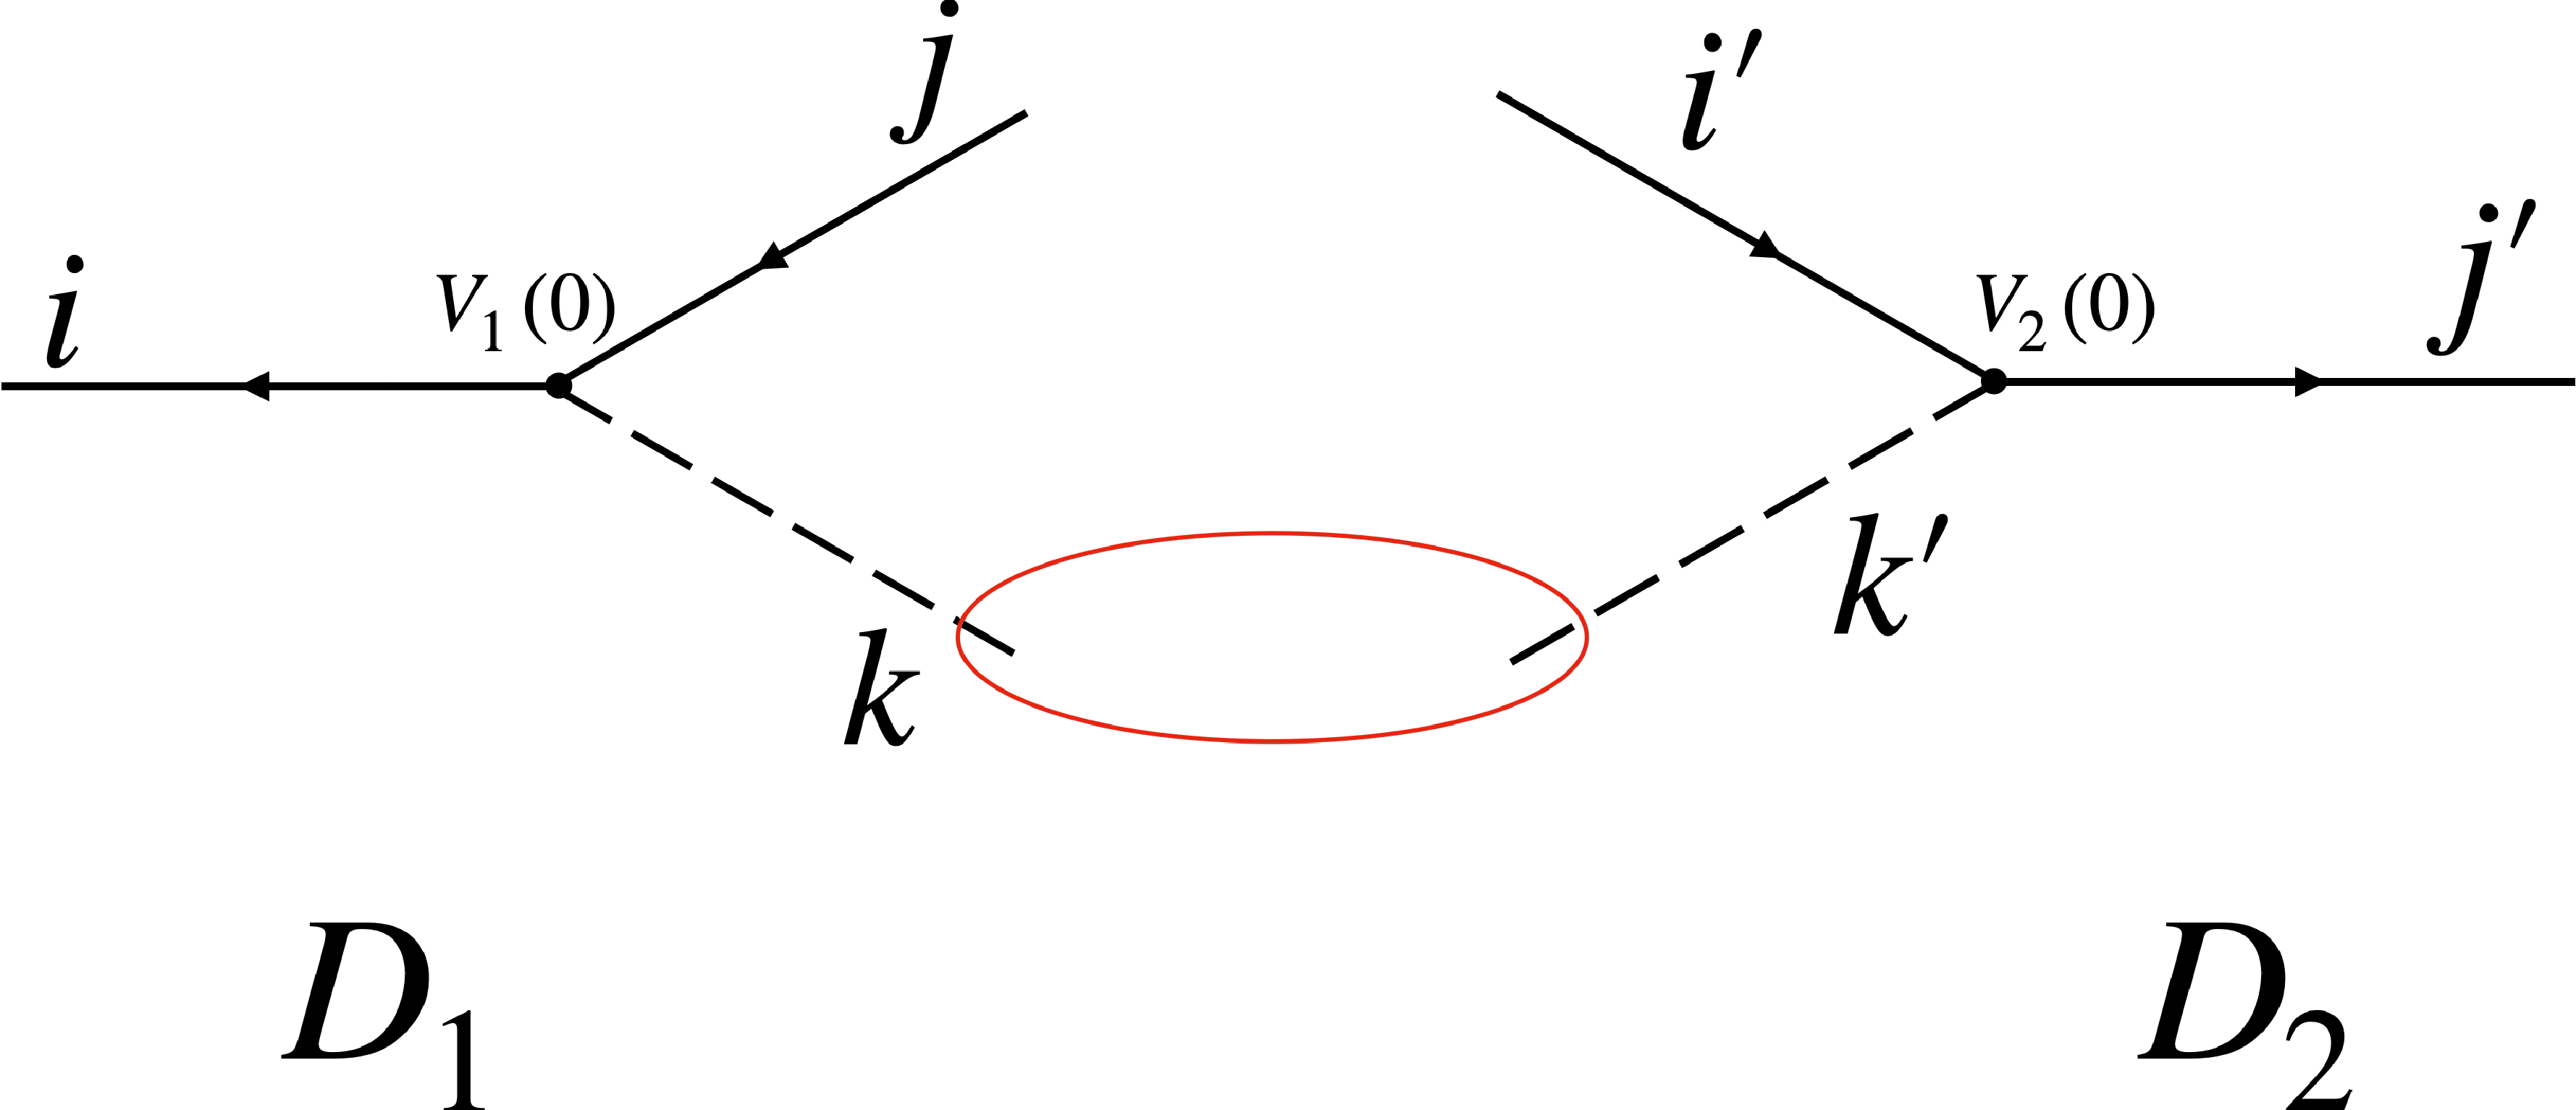
\includegraphics[width = 0.75\textwidth]{figures/D1D2.pdf}
    \caption{Two interaction diagrams, $D1$ and $D2$ are chosen. There is only one possible contraction, which is circled in red.}
    \label{fig:D1D2}
\end{figure}

\begin{figure}
    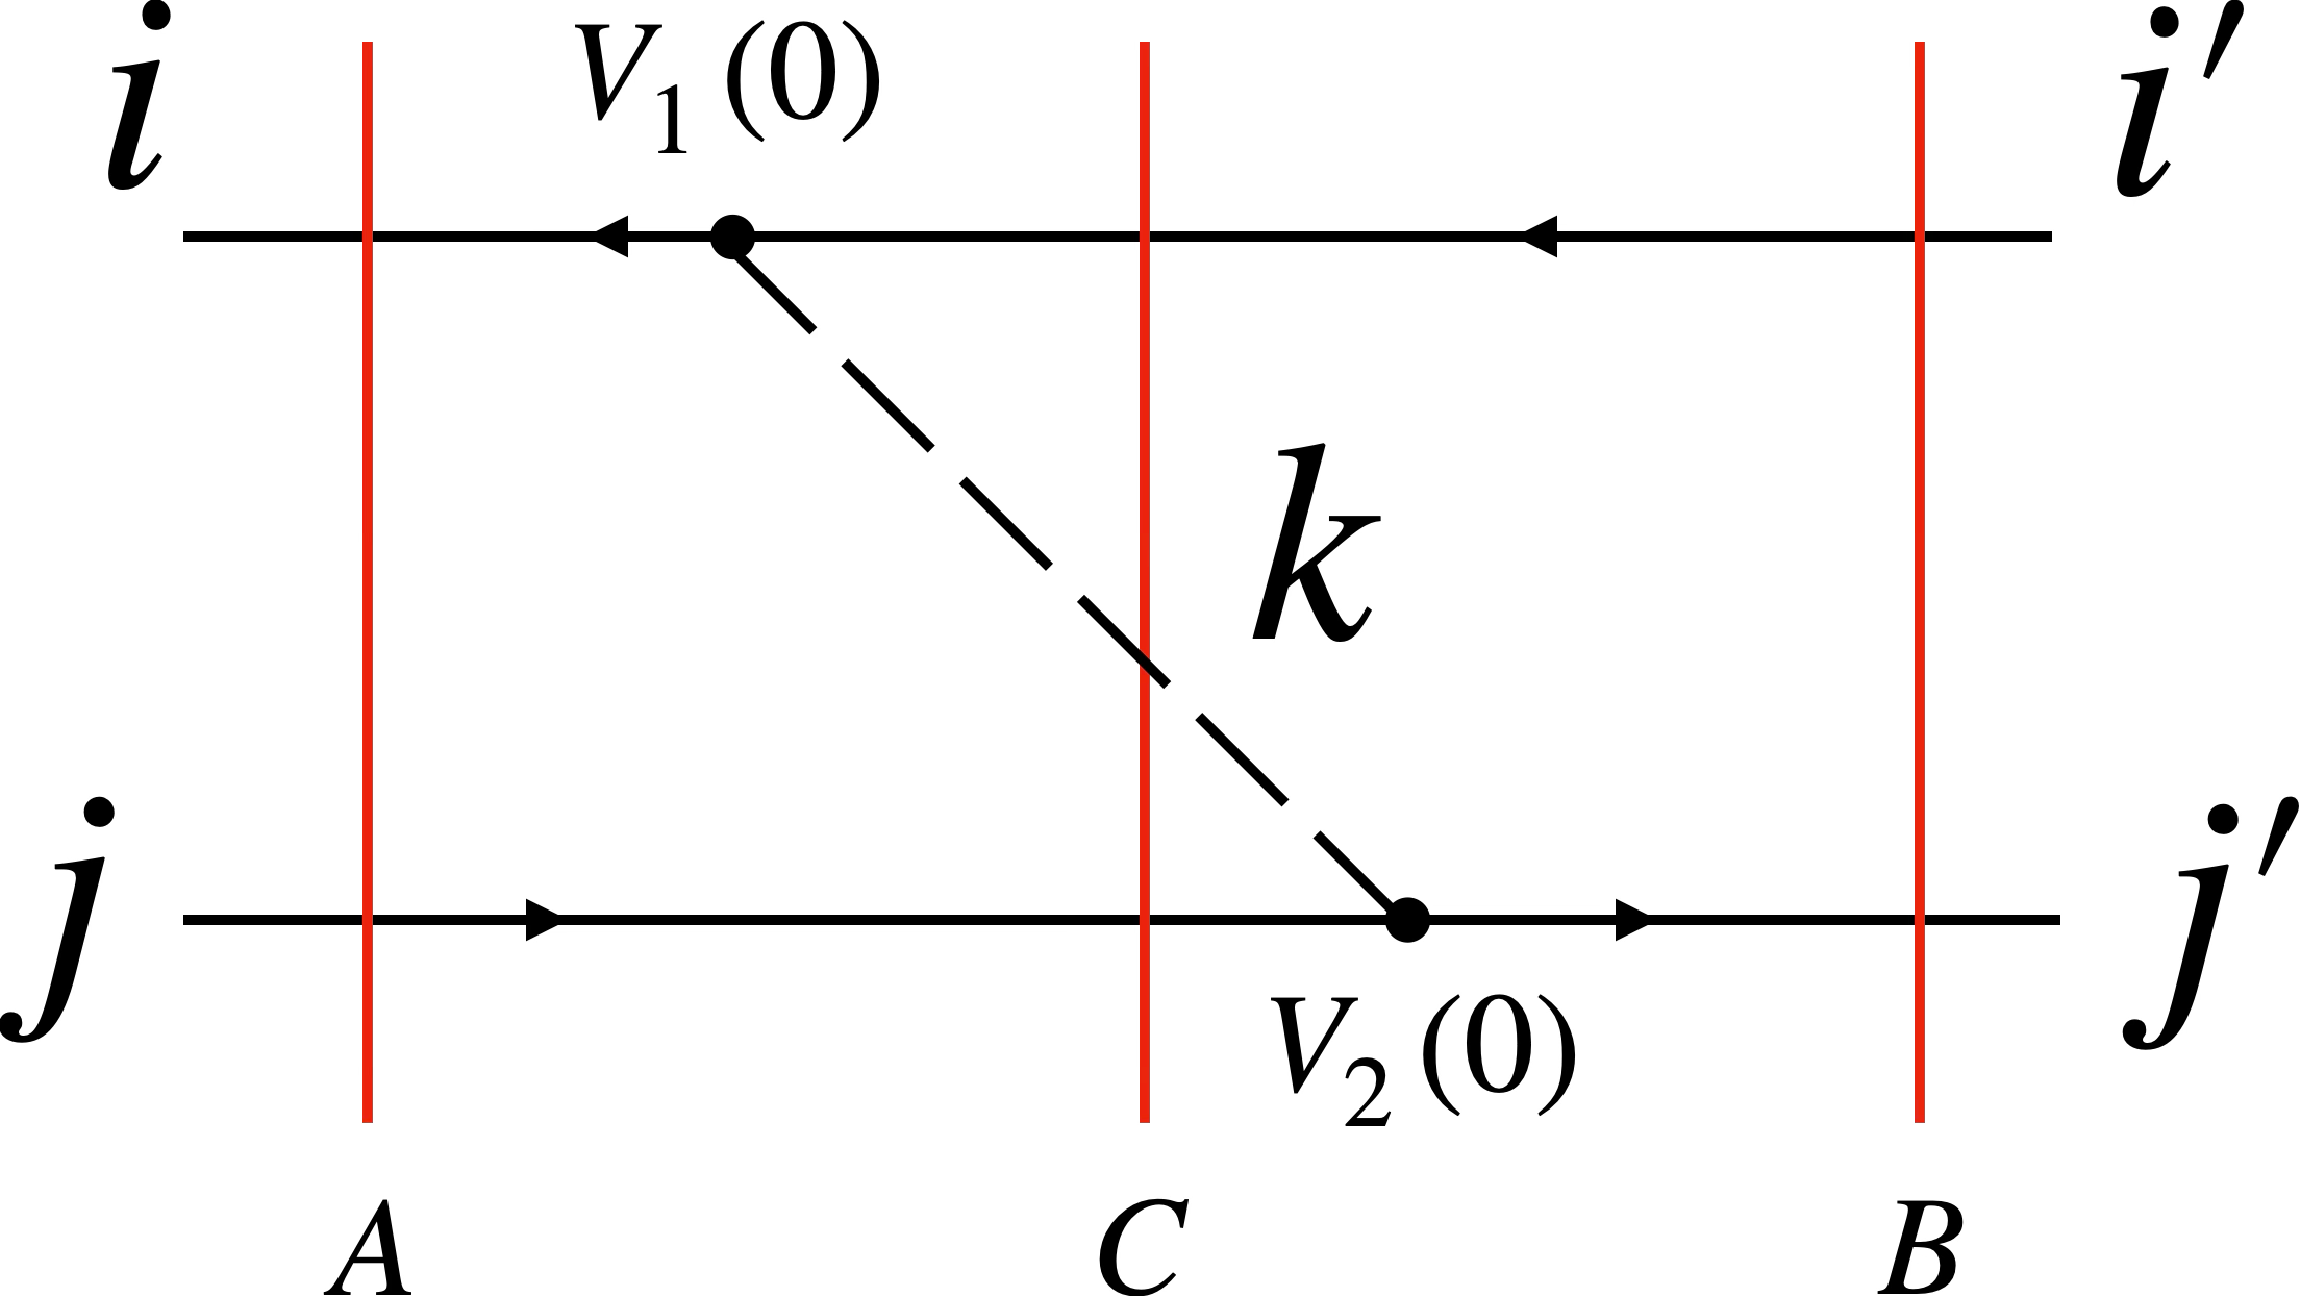
\includegraphics[width = 0.6\textwidth]{figures/contraction.pdf}
    \caption{When we contract the bosons in $D1$ and $D2$ in figure \ref{fig:D1D2}, we get an $\mathcal{O}(g^2)$ diagram. Keeping track of the original indices is unnecesssary, if you label them in a consistent way.}
    \label{fig:contraction}
\end{figure}

For this example, $\mathcal{P}_A + \mathcal{P}_B - 2\mathcal{P}_2 = c_i - c_{i'} + c_j - c_{j'} - 2c_k$ (i.e. $\mathcal{P}_i$ is the sum of momentum along the red line of $i$), and $V_1(t) = c_{ijk}(t), V_2(t) = \bar c^*_{ijk}(t)$. Thus, $$\left[\mathcal{G}^{(1)}(t), H^{(1)}(t) \right]_{D_1, D_2} = \int_{ijki'j'}\left(c_i - c_{i'} + c_j - c_{j'} - 2c_k \right)c_{ijk}(0)\bar c^*_{ijk}(0) b_i^\dagger b_{i'}d_j^\dagger d_{j'}.$$

Doing this $\forall D_1, D_2 \in \{interactions\}$, we obtain $\left[\mathcal{G}^{(1)}(t), H^{(1)}(t) \right]$. 
The important information obtained from computing all of the contractions is that you can now write down a parameterized form for $\mathcal{O}(g^2)$ terms to add to $H^{(2)}(t)$. 
Again, using the example of figures \ref{fig:D1D2} and \ref{fig:contraction}, we could parameterize this addition to $H^{(2)}(t)$ as $$H^{(2)}_{D_1, D_2}(t) = \int_{ijki'j'}K(t)  b_i^\dagger b_{i'}d_j^\dagger d_{j'},$$ where $K(t)$ is a parameterized coefficient to be determined by solving equation \ref{eq:rgpep-second-order}. \gus{Change $D1, D2$ subscript in above equation to be a figure of the corresponding diagram}.

Now that we have a parameterized form of $H^{(2)}(t)$, complete with additional terms from the contractions, we can calculate the first commutator in equation \ref{eq:rgpep-second-order}.

For a given term in $H^{(2)}(t)$, the commutator $\left[\left[H_0, g^2H^{(2)}(t)\right], H_0\right]$ is simple to calculate. 
In a similar way that $\left[\left[H_0, gH^{(1)}(t)\right], H_0\right]$ was calculated, this second order commutator will modify the given term by $-\left(\mathcal{P}_A - \mathcal{P}_B\right)^2$ (refer to figure \ref{fig:contraction}).

We can finally write down the general form of the differential equation that comes from equation \ref{eq:rgpep-second-order} for a given second order diagram $D$ with parameterized coefficient in $H^{(2)}(t)$, $K(t)$:

\begin{equation}
    \label{eq:second-order-DE}
    \frac{d}{dt}K_D(t) = -\left(\mathcal{P}_A - \mathcal{P}_B \right)^2 K_D(t) + \left(\mathcal{P}_A + \mathcal{P}_B - 2\mathcal{P}_C \right)V_1(0)e^{-p_{V_1}^2t}V_2(0)e^{-p_{V_2}^2t}
\end{equation}

where $p_{V_i}^2$ is sum of $c_j's$ into $V_i$ minus sum of $c_j's$ out of $V_i$. 
For the example of $D_1$ in figure \ref{fig:D1D2}, $p_{V_1} = \left(c_i - c_j - c_k \right)$.

The general solution to equation \ref{eq:second-order-DE} is \footnote{A differential equation of the form $\frac{dy}{dt} = -p(t)y(t) + q(t)$ has the general solution $y(t) = e^{-h(t)}\int e^{h(t)}q(t) + Ce^{-h(t)}$, where $h(t) = \int dt p(t)$}:

\begin{equation}
    K_D(t) = \frac{\left(\mathcal{P}_A + \mathcal{P}_B - 2\mathcal{P}_C \right)V_1(0)V_2(0)}{p_{V_1}^2 + p_{V_2}^2 - \left(\mathcal{P}_A - \mathcal{P}_B \right)^2} \left(e^{-\left( \mathcal{P}_A - \mathcal{P}_B\right)^2t} - e^{-\left(p_{V_1}^2 + p_{V_2}^2\right)t} \right) + K_D(0)
\end{equation}

The last thing to note before writing out the solution to \ref{eq:rgpep-second-order} is that we must take into account the original instantaneous second order diagrams present in \ref{eq:yukawa-hamiltonian}. 
The first commutator in \ref{eq:rgpep-second-order} will be non-zero for this interaction, and can simply be wrote down as the original term, modified by $-\left(\mathcal{P}_A - \mathcal{P}_B \right)^2$. 
Each second order term in the Hamiltonian is now written out explicitly in table \ref{tab:H2}:


\begin{table}[h]
    \centering
    \hspace*{-1.7cm} % Move table to the left
    \begin{tabular}{|c|c|}
        \hline
        \textbf{Diagram ($D$)} & \textbf{$H_D^{(2)}(t)$} \\
        \hline
        \hline
        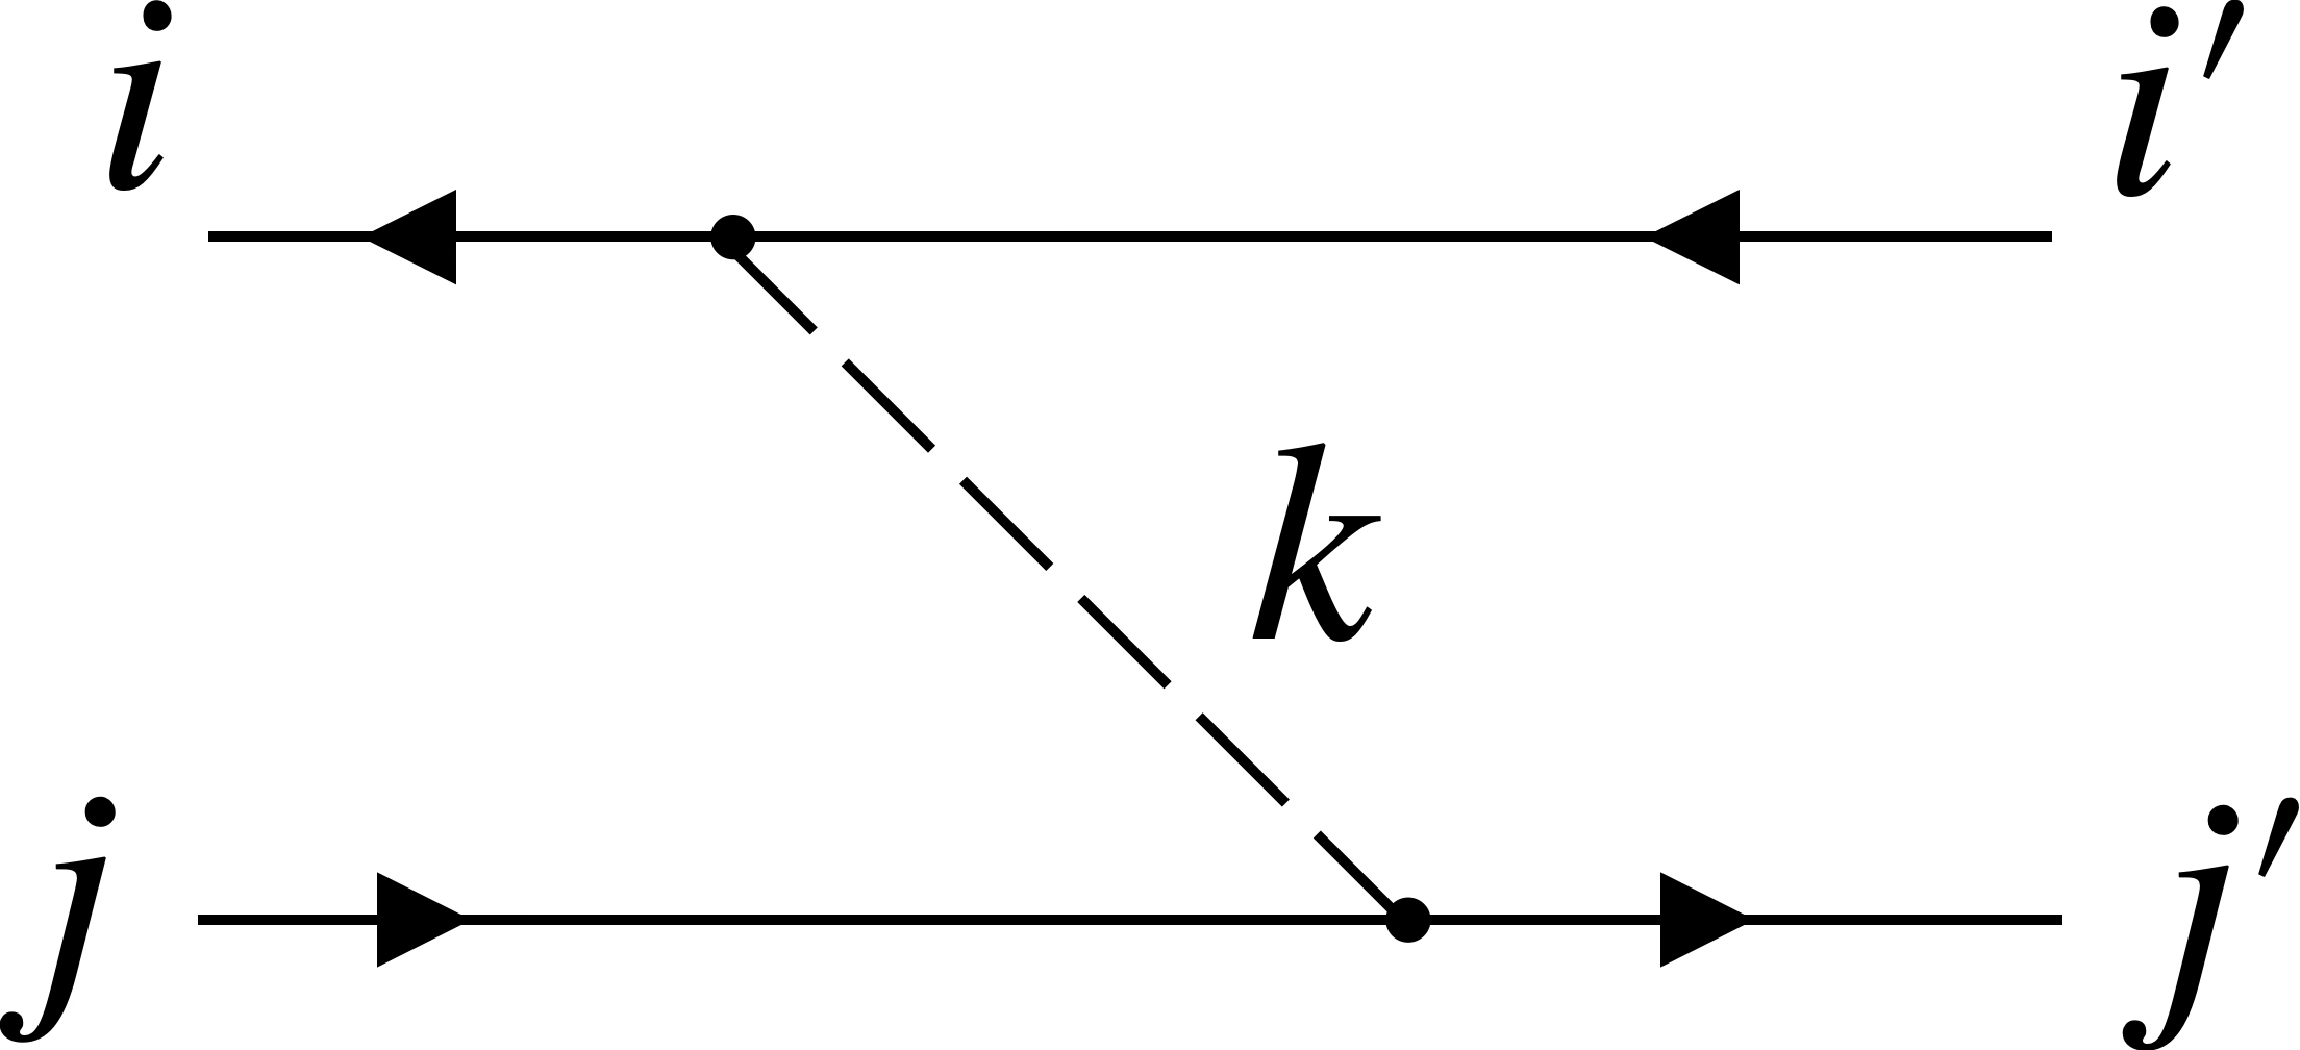
\includegraphics[width=0.15\textwidth]{figures/ffbar-ffbar(1).pdf} & 
        {\small $\displaystyle 
        \int_{ijki'j'} \frac{(c_i + c_{j'} - c_{i'} - c_j - 2c_k)c_{ii'k}(0)\bar c^*_{jj'k}(0)}
        {(c_i - c_{i'} - c_k)^2 + (c_j + c_k - c_{j'})^2 - (c_i + c_j - c_{i'} - c_{j'})^2}
        \left( e^{- (c_i + c_j - c_{i'} - c_{j'})^2t} 
        - e^{-\left( (c_i - c_{i'} - c_k)^2 + (c_j + c_k - c_{j'})^2 \right)t} \right)
        b_i^\dagger b_{i'} d_j^\dagger d_{j'}
        $} \\
        \hline
        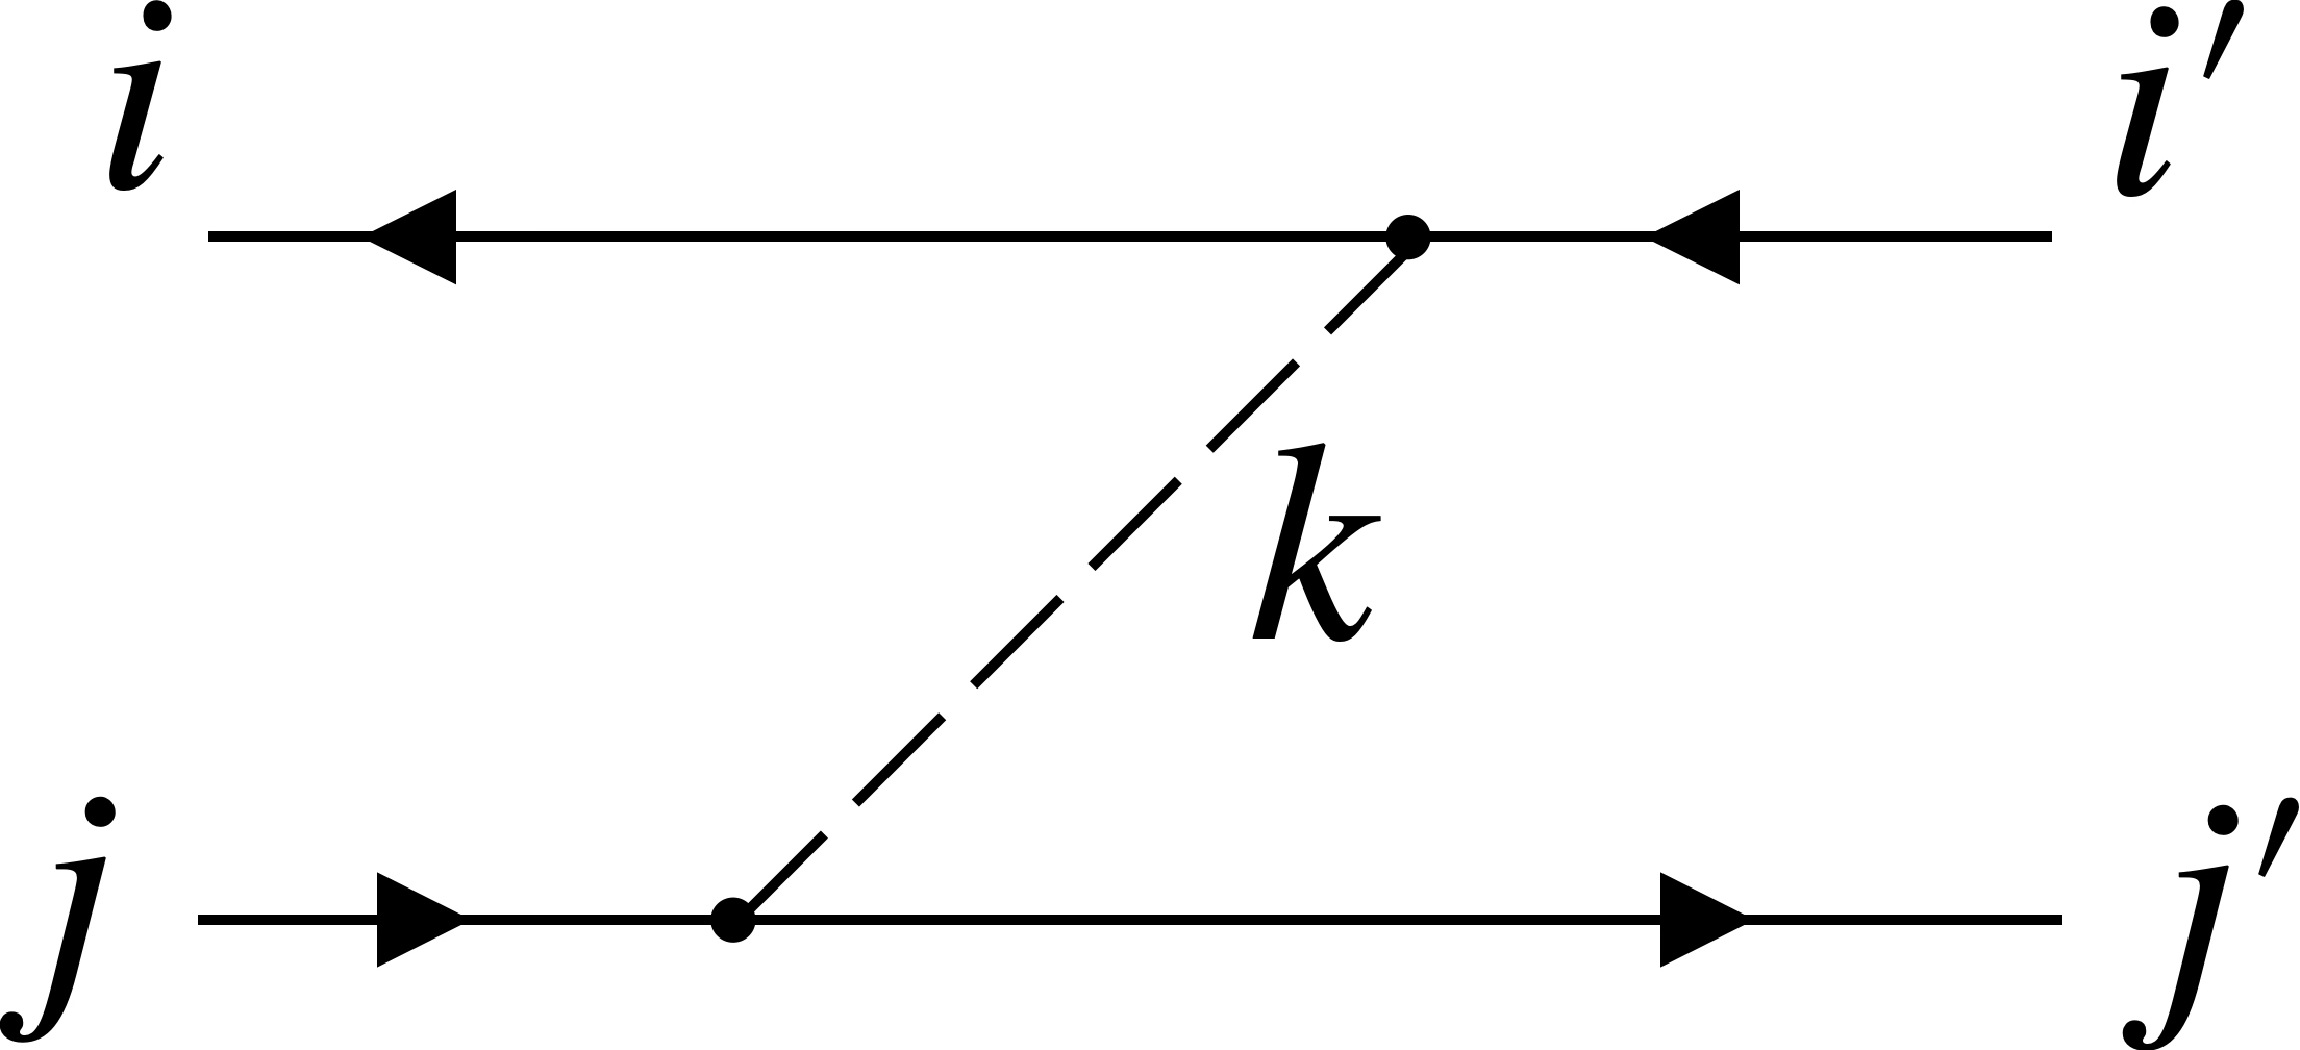
\includegraphics[width=0.15\textwidth]{figures/ffbar-ffbar(2).pdf} & 
        {\small $\displaystyle 
        \int_{ijki'j'} \frac{(c_{i'} + c_{j} -c_i  - c_{j'} - 2c_k)c^*_{ii'k}(0)\bar c_{jj'k}(0)}
        {(c_i + c_k - c_{i'} )^2 + (c_j - c_{j'}- c_k )^2 - (c_i + c_j - c_{i'} - c_{j'})^2}
        \left( e^{- (c_i + c_j - c_{i'} - c_{j'})^2t} 
        - e^{-\left( (c_i + c_k - c_{i'} )^2 + (c_j - c_{j'}- c_k )^2 \right)t} \right)
        b_i^\dagger b_{i'} d_j^\dagger d_{j'}
        $} \\
        \hline
        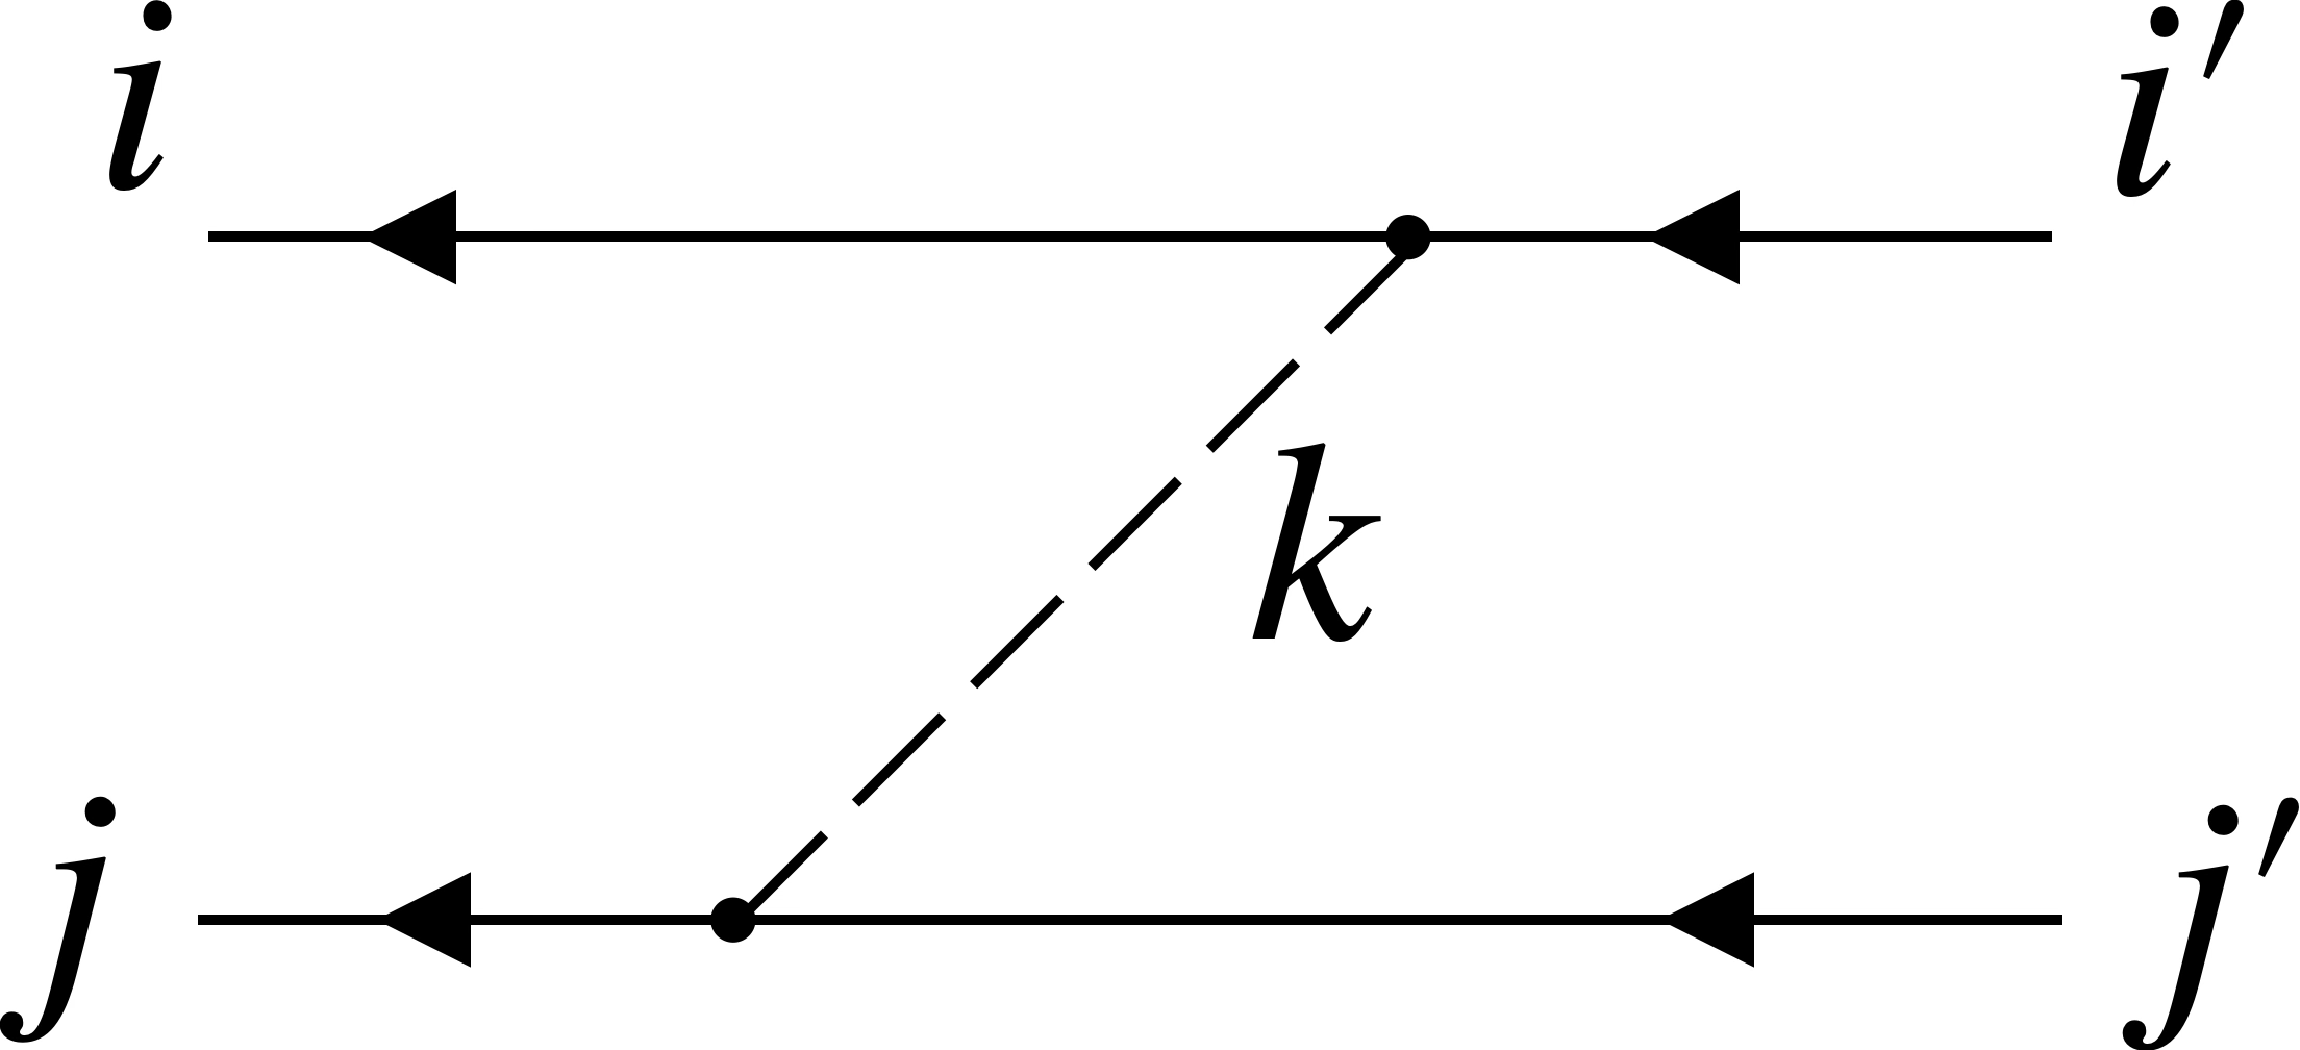
\includegraphics[width=0.15\textwidth]{figures/ff-ff.pdf} & 
        {\small $\displaystyle 
        \int_{ijki'j'} \frac{(c_{i'} + c_{j} -c_i  - c_{j'} - 2c_k)c^*_{ii'k}(0)c_{jj'k}(0)}
        {(c_i + c_k - c_{i'} )^2 + (c_j - c_{j'}- c_k )^2 - (c_i + c_j - c_{i'} - c_{j'})^2}
        \left( e^{- (c_i + c_j - c_{i'} - c_{j'})^2t} 
        - e^{-\left( (c_i + c_k - c_{i'} )^2 + (c_j - c_{j'}- c_k )^2 \right)t} \right)
        b_i^\dagger b_j^\dagger b_{i'}  b_{j'}
        $} \\
        \hline
        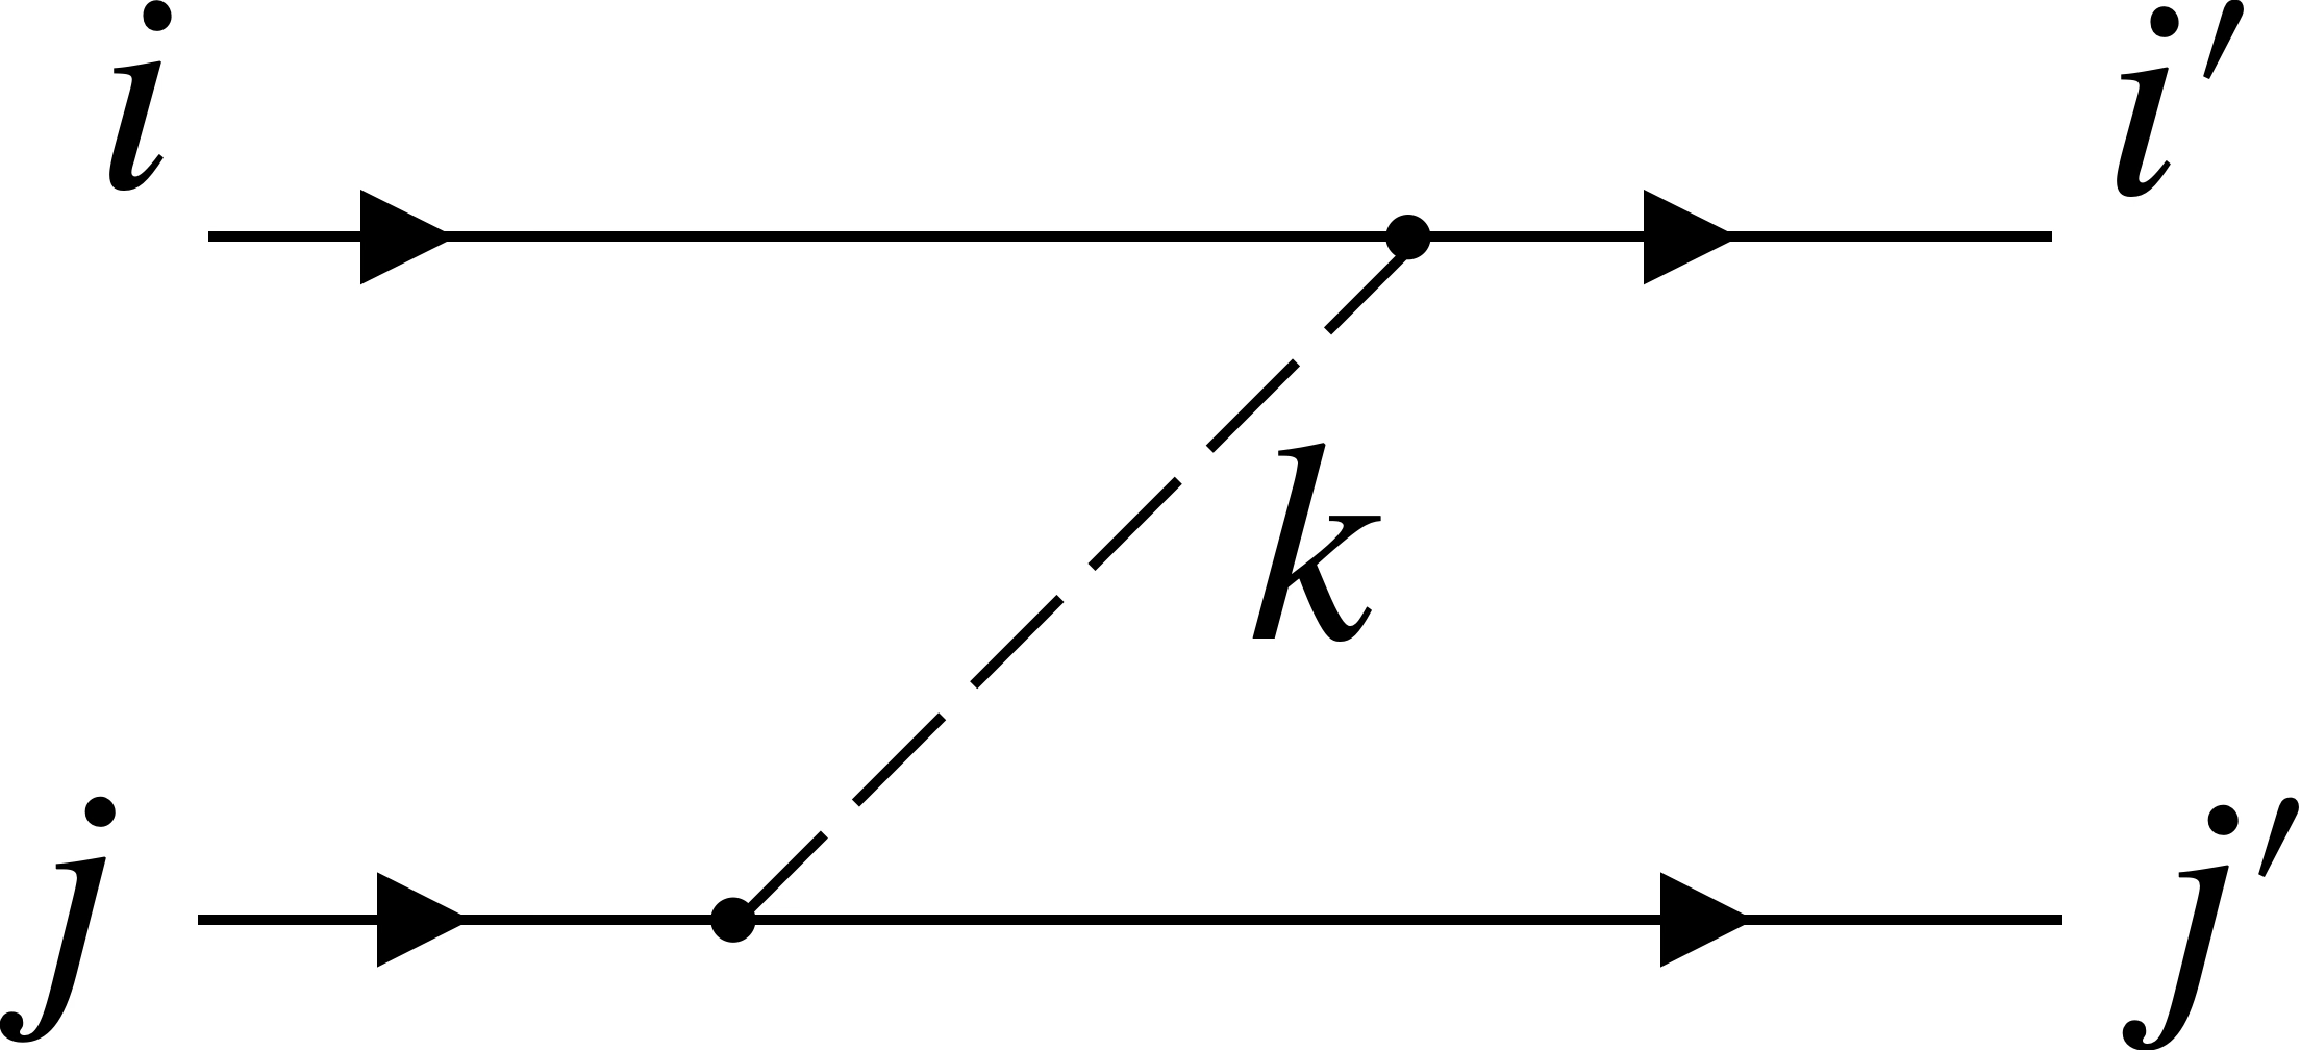
\includegraphics[width=0.15\textwidth]{figures/fbarfbar-fbarfbar.pdf} & 
        {\small $\displaystyle 
        \int_{ijki'j'} \frac{(c_{i'} + c_{j} -c_i  - c_{j'} - 2c_k)\bar c^*_{ii'k}(0)\bar c_{jj'k}(0)}
        {(c_i + c_k - c_{i'} )^2 + (c_j - c_{j'}- c_k )^2 - (c_i + c_j - c_{i'} - c_{j'})^2}
        \left( e^{- (c_i + c_j - c_{i'} - c_{j'})^2t} 
        - e^{-\left( (c_i + c_k - c_{i'} )^2 + (c_j - c_{j'}- c_k )^2 \right)t} \right)
        d_i^\dagger d_j^\dagger d_{i'}  d_{j'}
        $} \\
        \hline
        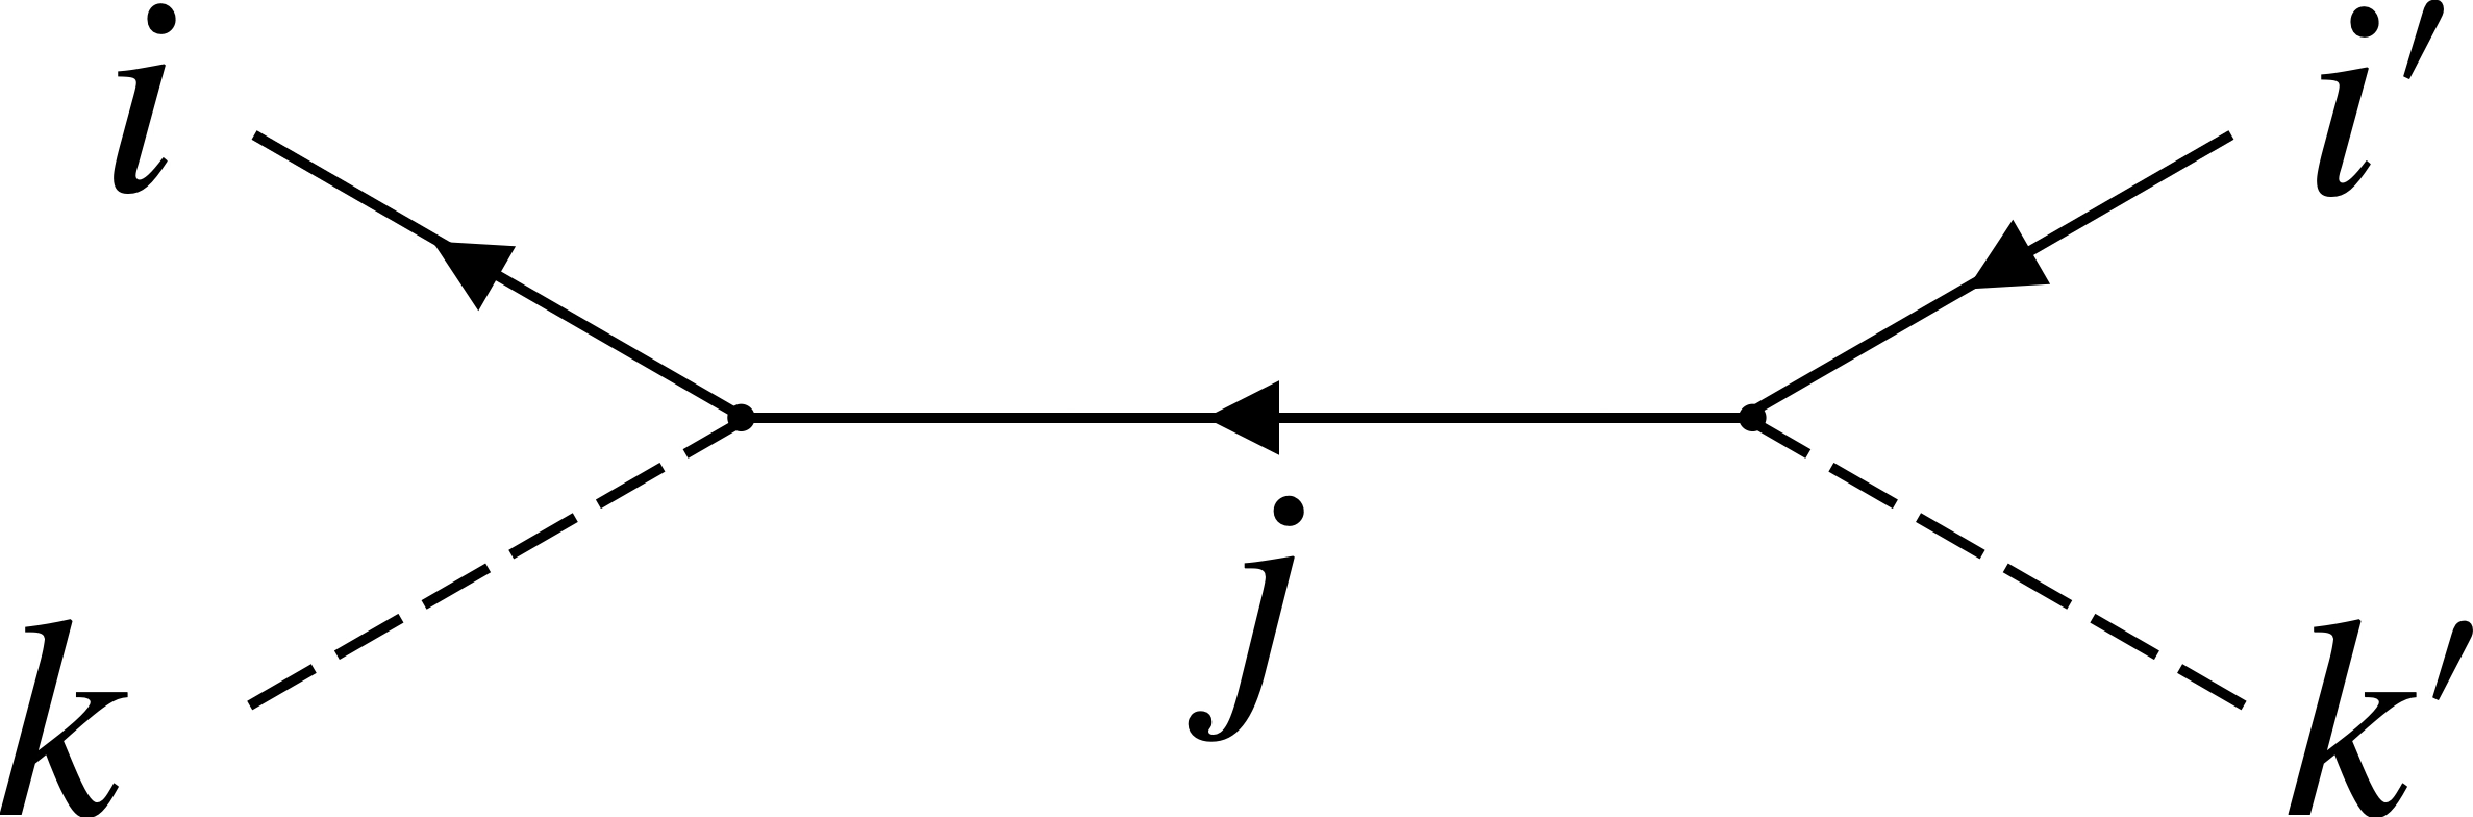
\includegraphics[width=0.15\textwidth]{figures/fb-fb.pdf} & 
        {\small $\displaystyle 
        \int_{ijki'k'} \frac{(c_i + c_{i'} + c_{k'} +c_k  - 2c_j) c^*_{ikj}(0) c_{ji'k'}(0)}
        {(c_i + c_k - c_{j} )^2 + (c_j - c_{i'}- c_{k'} )^2 - (c_i + c_k - c_{i'} - c_{k'})^2}
        \left( e^{- (c_i + c_k - c_{i'} - c_{k'})^2t} 
        - e^{-\left( (c_i + c_k - c_{j} )^2 + (c_j - c_{i'}- c_{k'} )^2 \right)t} \right)
        b_i^\dagger b_{i'}  a_k^\dagger a_{k'}
        $} \\
        \hline
        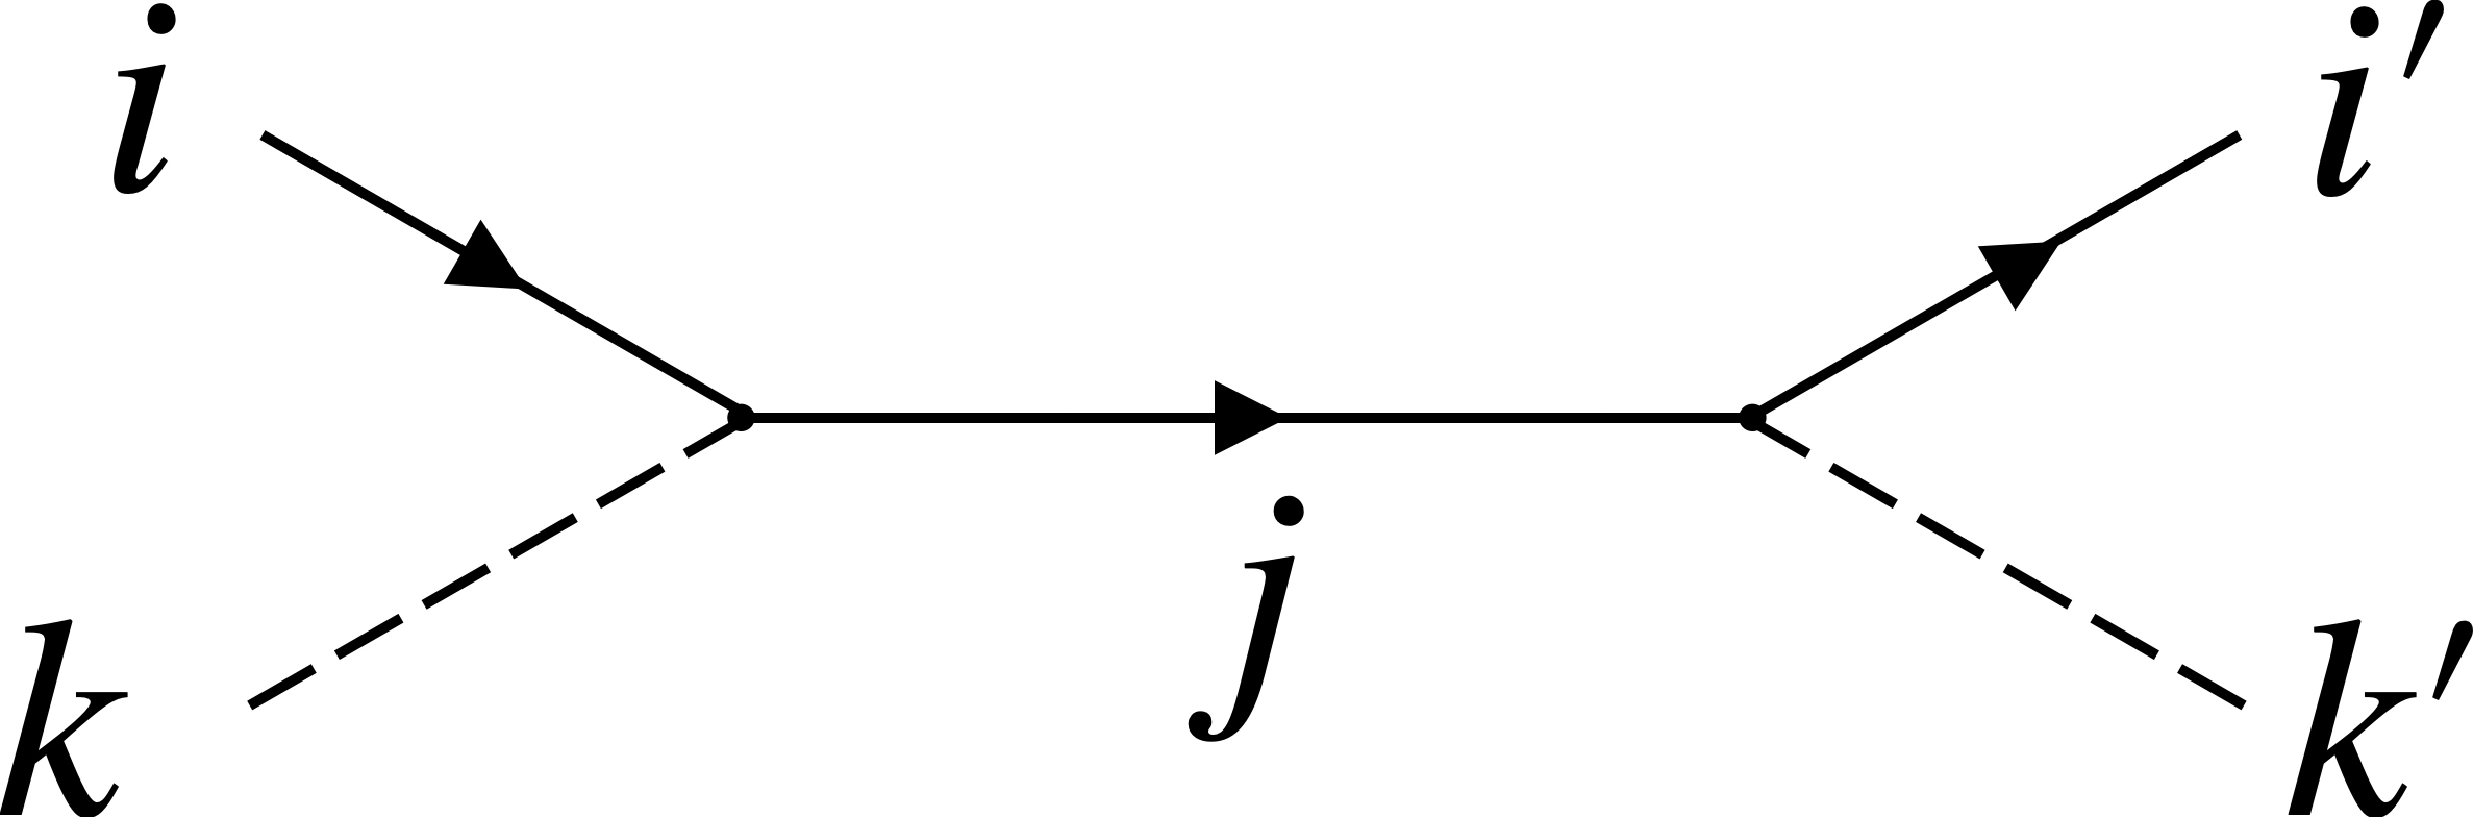
\includegraphics[width=0.15\textwidth]{figures/fbarb-fbarb.pdf} & 
        {\small $\displaystyle 
        \int_{ijki'k'} \frac{(c_i + c_{i'} + c_{k'} +c_k  - 2c_j) \bar c^*_{ikj}(0)\bar c_{ji'k'}(0)}
        {(c_i + c_k - c_{j} )^2 + (c_j - c_{i'}- c_{k'} )^2 - (c_i + c_k - c_{i'} - c_{k'})^2}
        \left( e^{- (c_i + c_k - c_{i'} - c_{k'})^2t} 
        - e^{-\left( (c_i + c_k - c_{j} )^2 + (c_j - c_{i'}- c_{k'} )^2 \right)t} \right)
        d_i^\dagger d_{i'}  a_k^\dagger a_{k'}
        $} \\
        \hline
        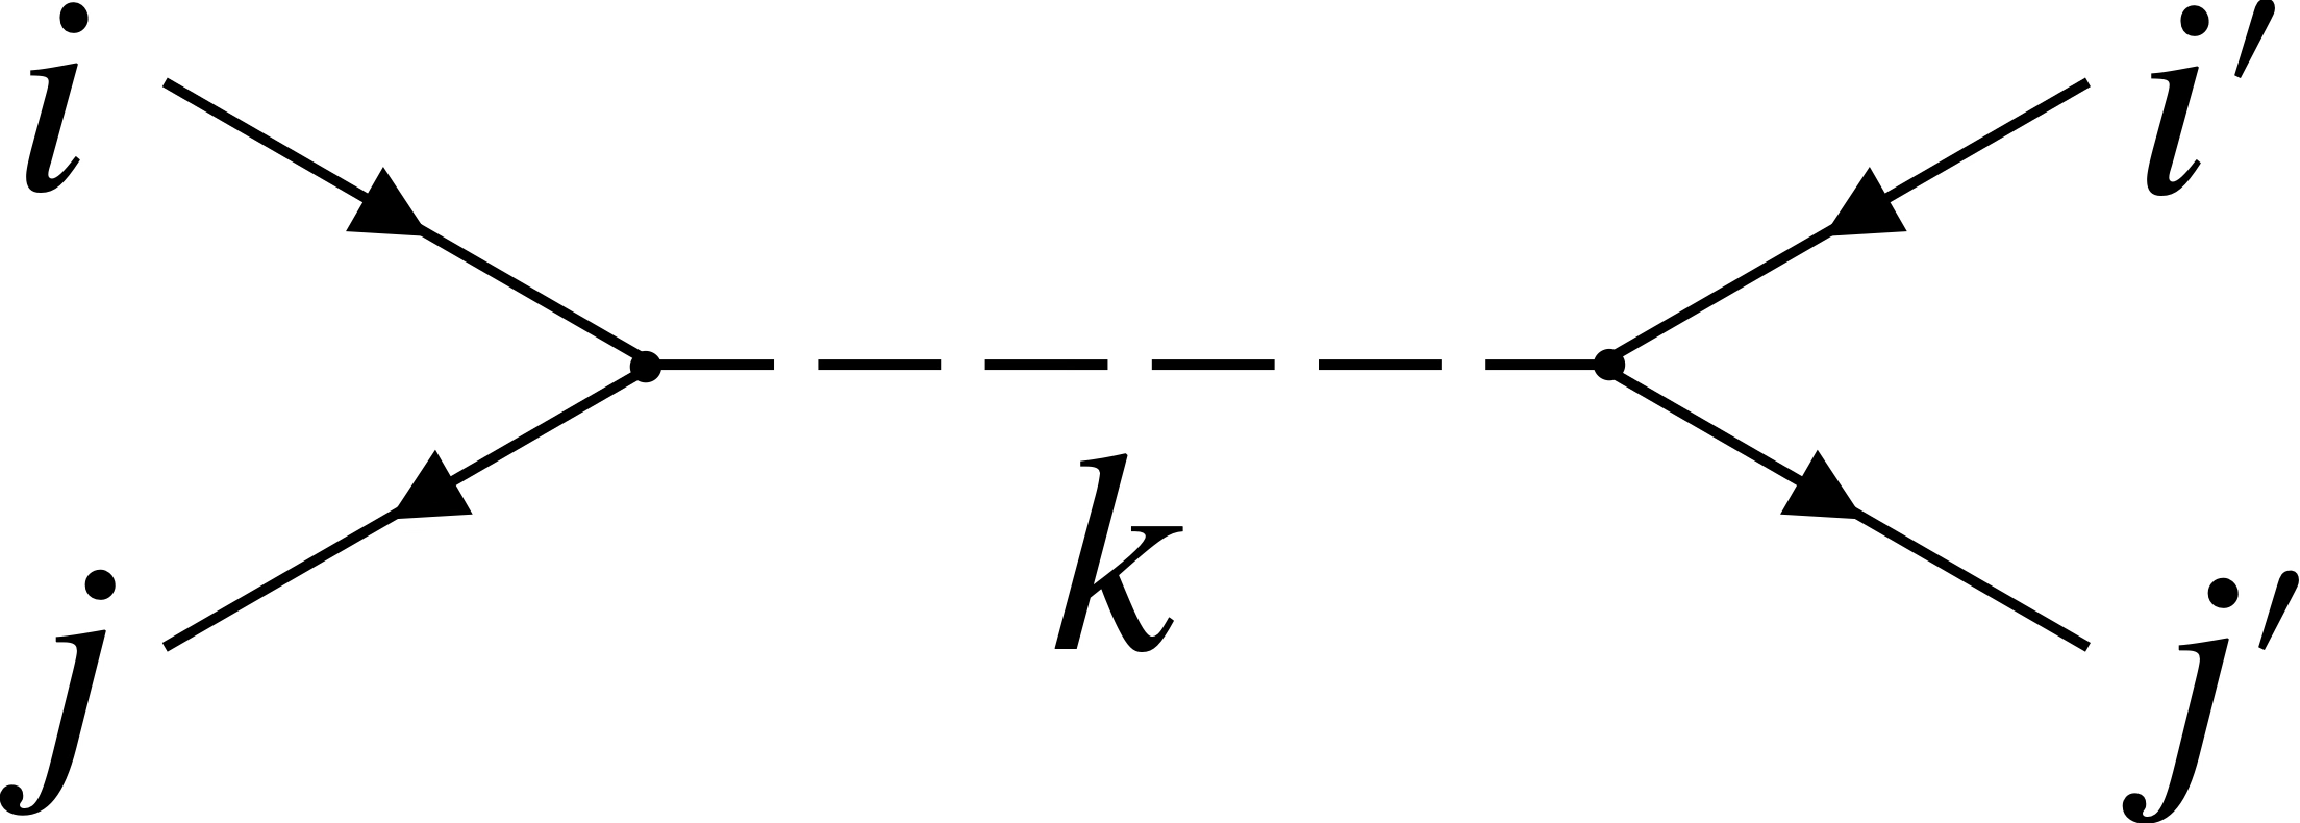
\includegraphics[width=0.15\textwidth]{figures/ffbar-ffbar(3).pdf} & 
        {\small $\displaystyle 
        \int_{ijki'k'} \frac{(c_i + c_{i'} + c_{j'} +c_j  - 2c_k) \tilde c_{ijk}(0)\tilde c^*_{ki'j'}(0)}
        {(c_i + c_j - c_{k} )^2 + (c_k - c_{i'}- c_{j'} )^2 - (c_i + c_j - c_{i'} - c_{j'})^2}
        \left( e^{- (c_i + c_j - c_{i'} - c_{j'})^2t} 
        - e^{-\left( (c_i + c_j - c_{k} )^2 + (c_k - c_{i'}- c_{j'} )^2\right)t} \right)
        b_i^\dagger b_{i'} d_j^\dagger d_{j'}
        $} \\
        \hline
        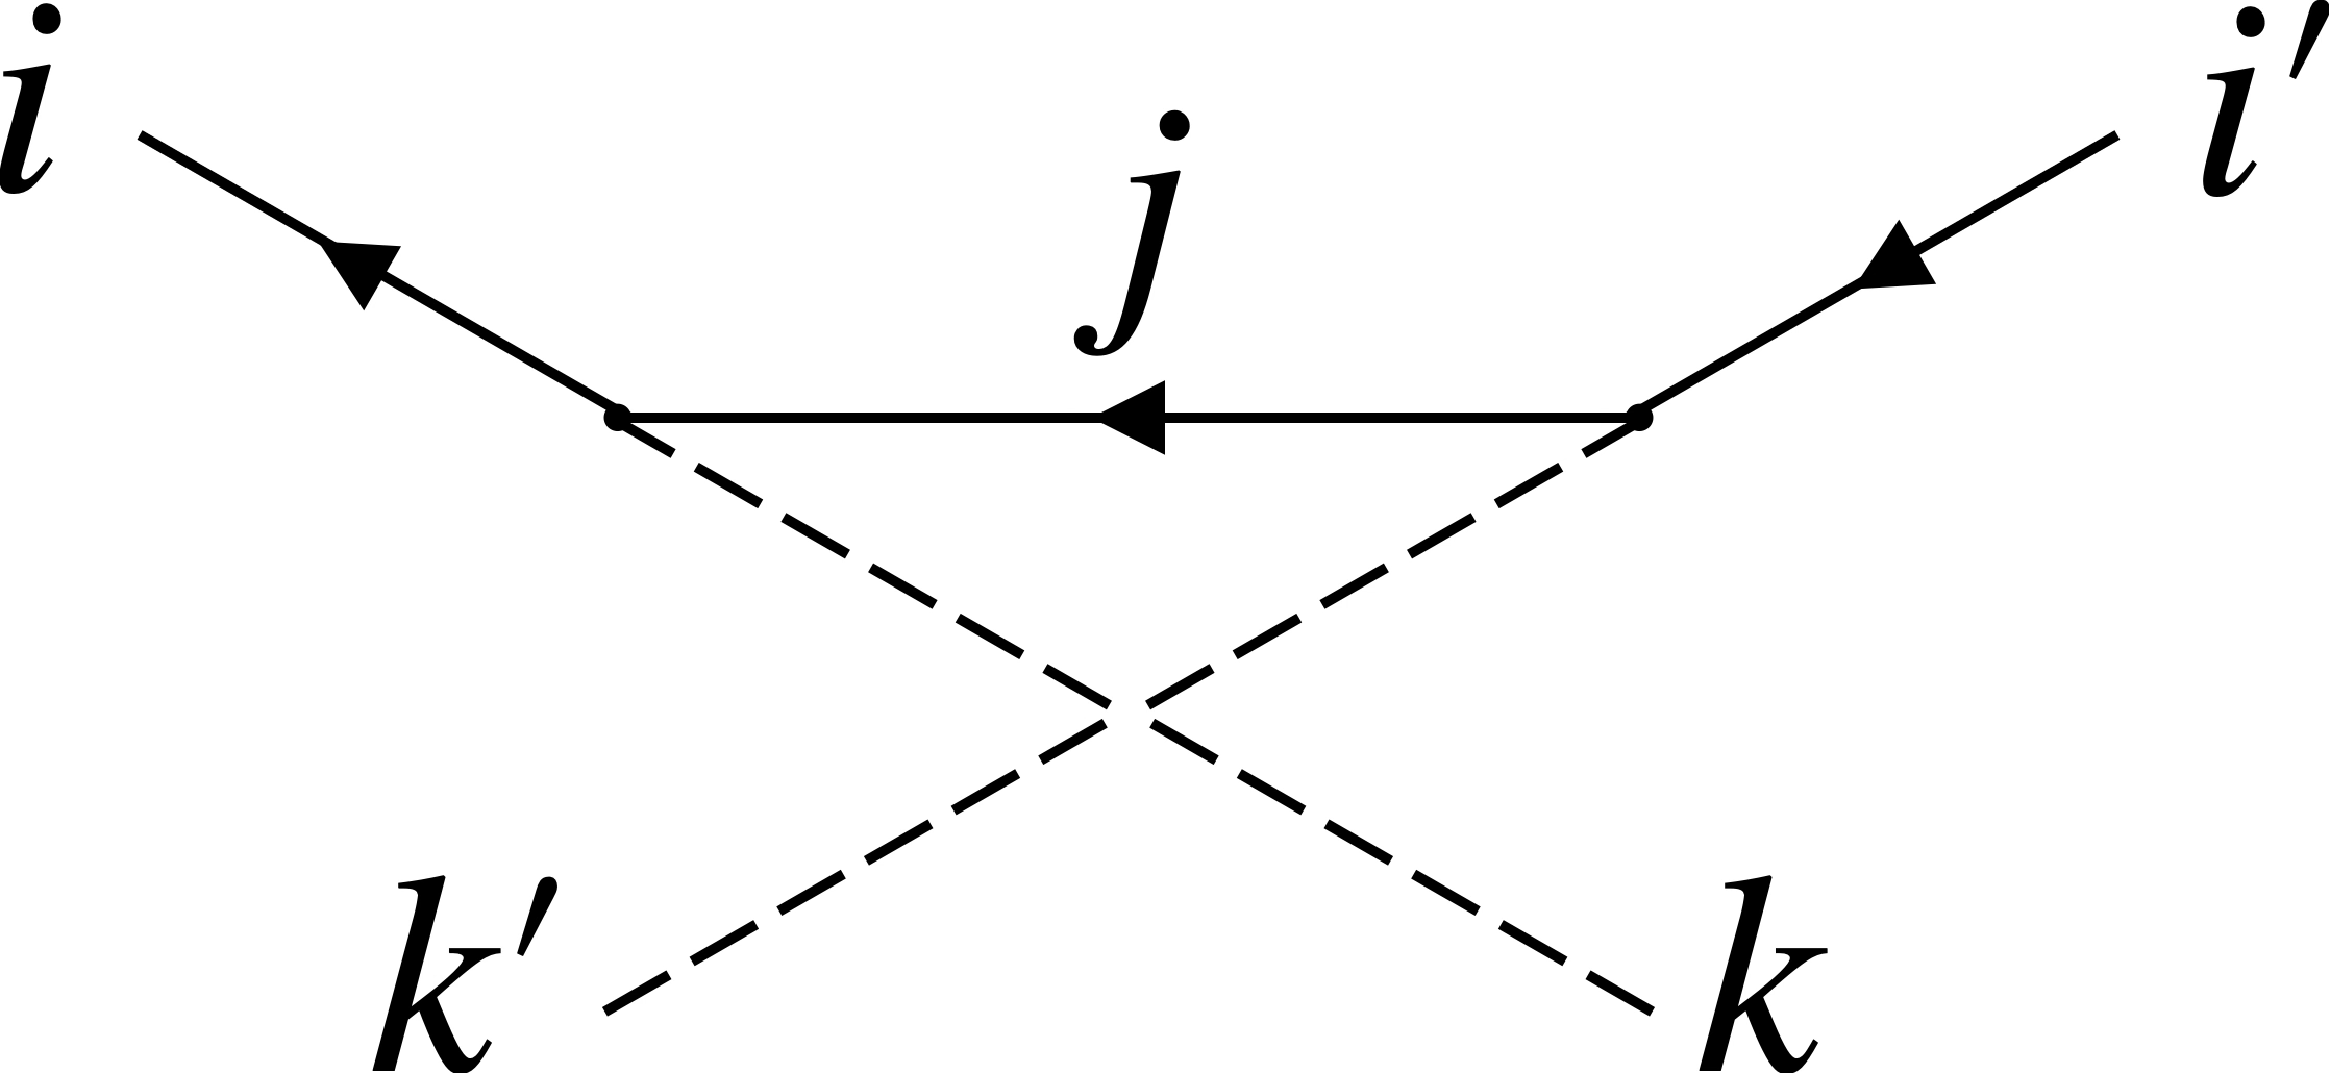
\includegraphics[width=0.15\textwidth]{figures/fb-fb(2).pdf} & 
        {\small $\displaystyle 
        \int_{ijki'k'} \frac{(c_i + c_{i'}-c_k - c_{k'}   - 2c_j)  c_{ijk}(0) c^*_{jk'i'}(0)}
        {(c_i - c_k - c_{j} )^2 + (c_j+ c_{k'} - c_{i'} )^2 - (c_i + c_{k'} - c_{i'} - c_{k})^2}
        \left( e^{- (c_i + c_{k'} - c_{i'} - c_{k})^2t} 
        - e^{-\left( (c_i - c_k - c_{j} )^2 + (c_j+ c_{k'} - c_{i'} )^2 \right)t} \right)
        b_i^\dagger b_{i'}   a_{k'}^\dagger a_k
        $} \\
        \hline
        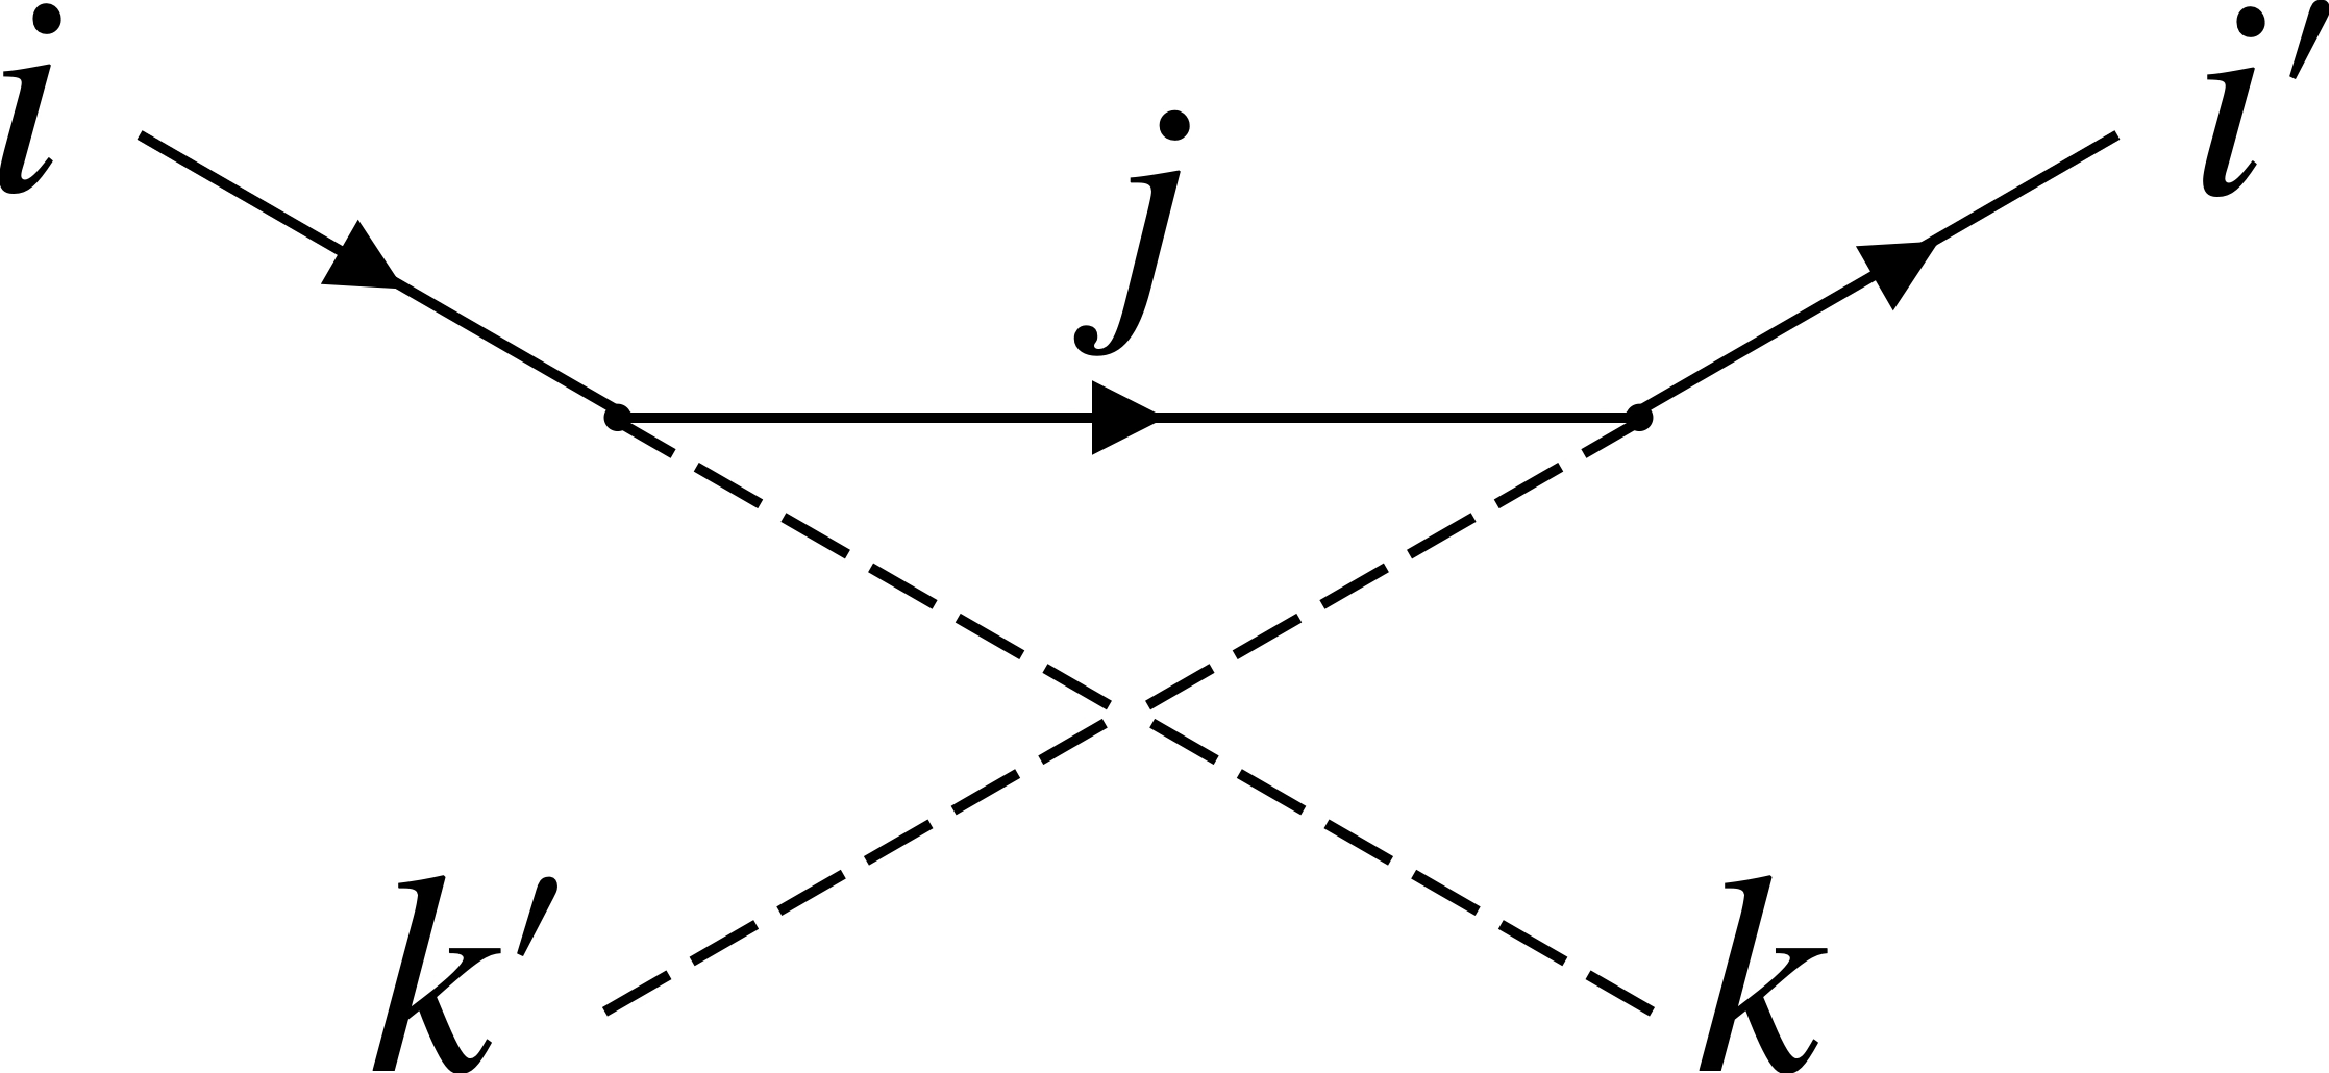
\includegraphics[width=0.15\textwidth]{figures/fbarb-fbarb(2).pdf} & 
        {\small $\displaystyle 
        \int_{ijki'k'} \frac{(c_i + c_{i'}-c_k - c_{k'}   - 2c_j)  \bar c_{ijk}(0) \bar c^*_{jk'i'}(0)}
        {(c_i - c_k - c_{j} )^2 + (c_j+ c_{k'} - c_{i'} )^2 - (c_i + c_{k'} - c_{i'} - c_{k})^2}
        \left( e^{- (c_i + c_{k'} - c_{i'} - c_{k})^2t} 
        - e^{-\left( (c_i - c_k - c_{j} )^2 + (c_j+ c_{k'} - c_{i'} )^2 \right)t} \right)
        d_i^\dagger d_{i'}   a_{k'}^\dagger a_k
        $} \\
        \hline
        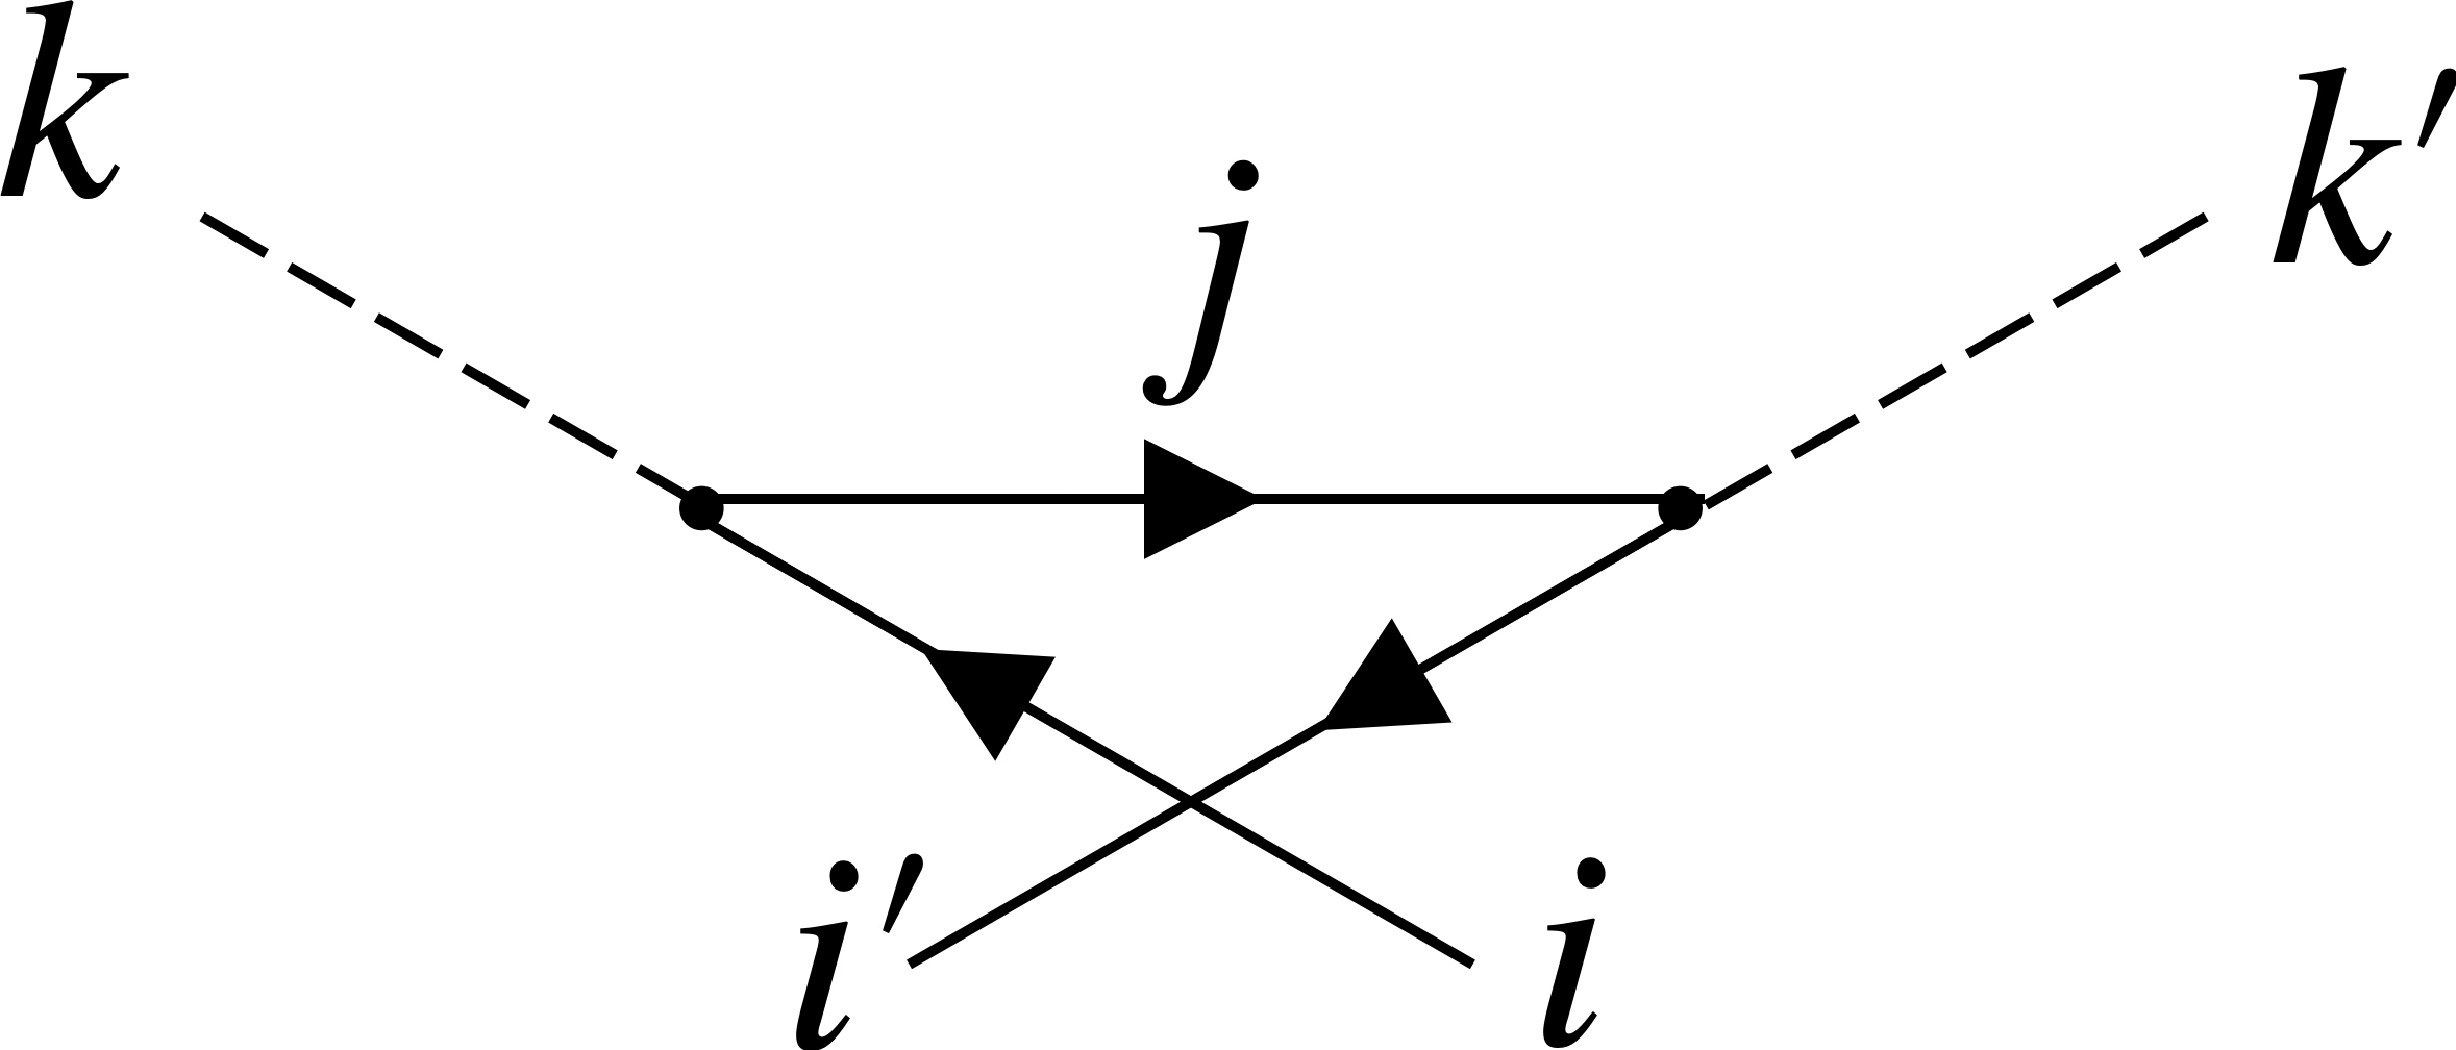
\includegraphics[width=0.15\textwidth]{figures/bf-bf.pdf} & 
        {\small $\displaystyle 
        \int_{ijki'k'} \frac{(c_k + c_{k'}-c_i - c_{i'}   - 2c_j)  \tilde c_{i'jk'}(0) \tilde c^*_{kij}(0)}
        {(c_{i'} + c_j - c_{k'} )^2 + (c_k- c_{i} - c_{j} )^2 - (c_{i'} + c_{k} - c_{i} - c_{k'})^2}
        \left( e^{- (c_{i'} + c_{k} - c_{i} - c_{k'})^2t} 
        - e^{-\left((c_{i'} + c_j - c_{k'} )^2 + (c_k- c_{i} - c_{j} )^2 \right)t} \right)
        d_{i'}^\dagger d_{i}   a_{k}^\dagger a_{k'}
        $} \\
        \hline
        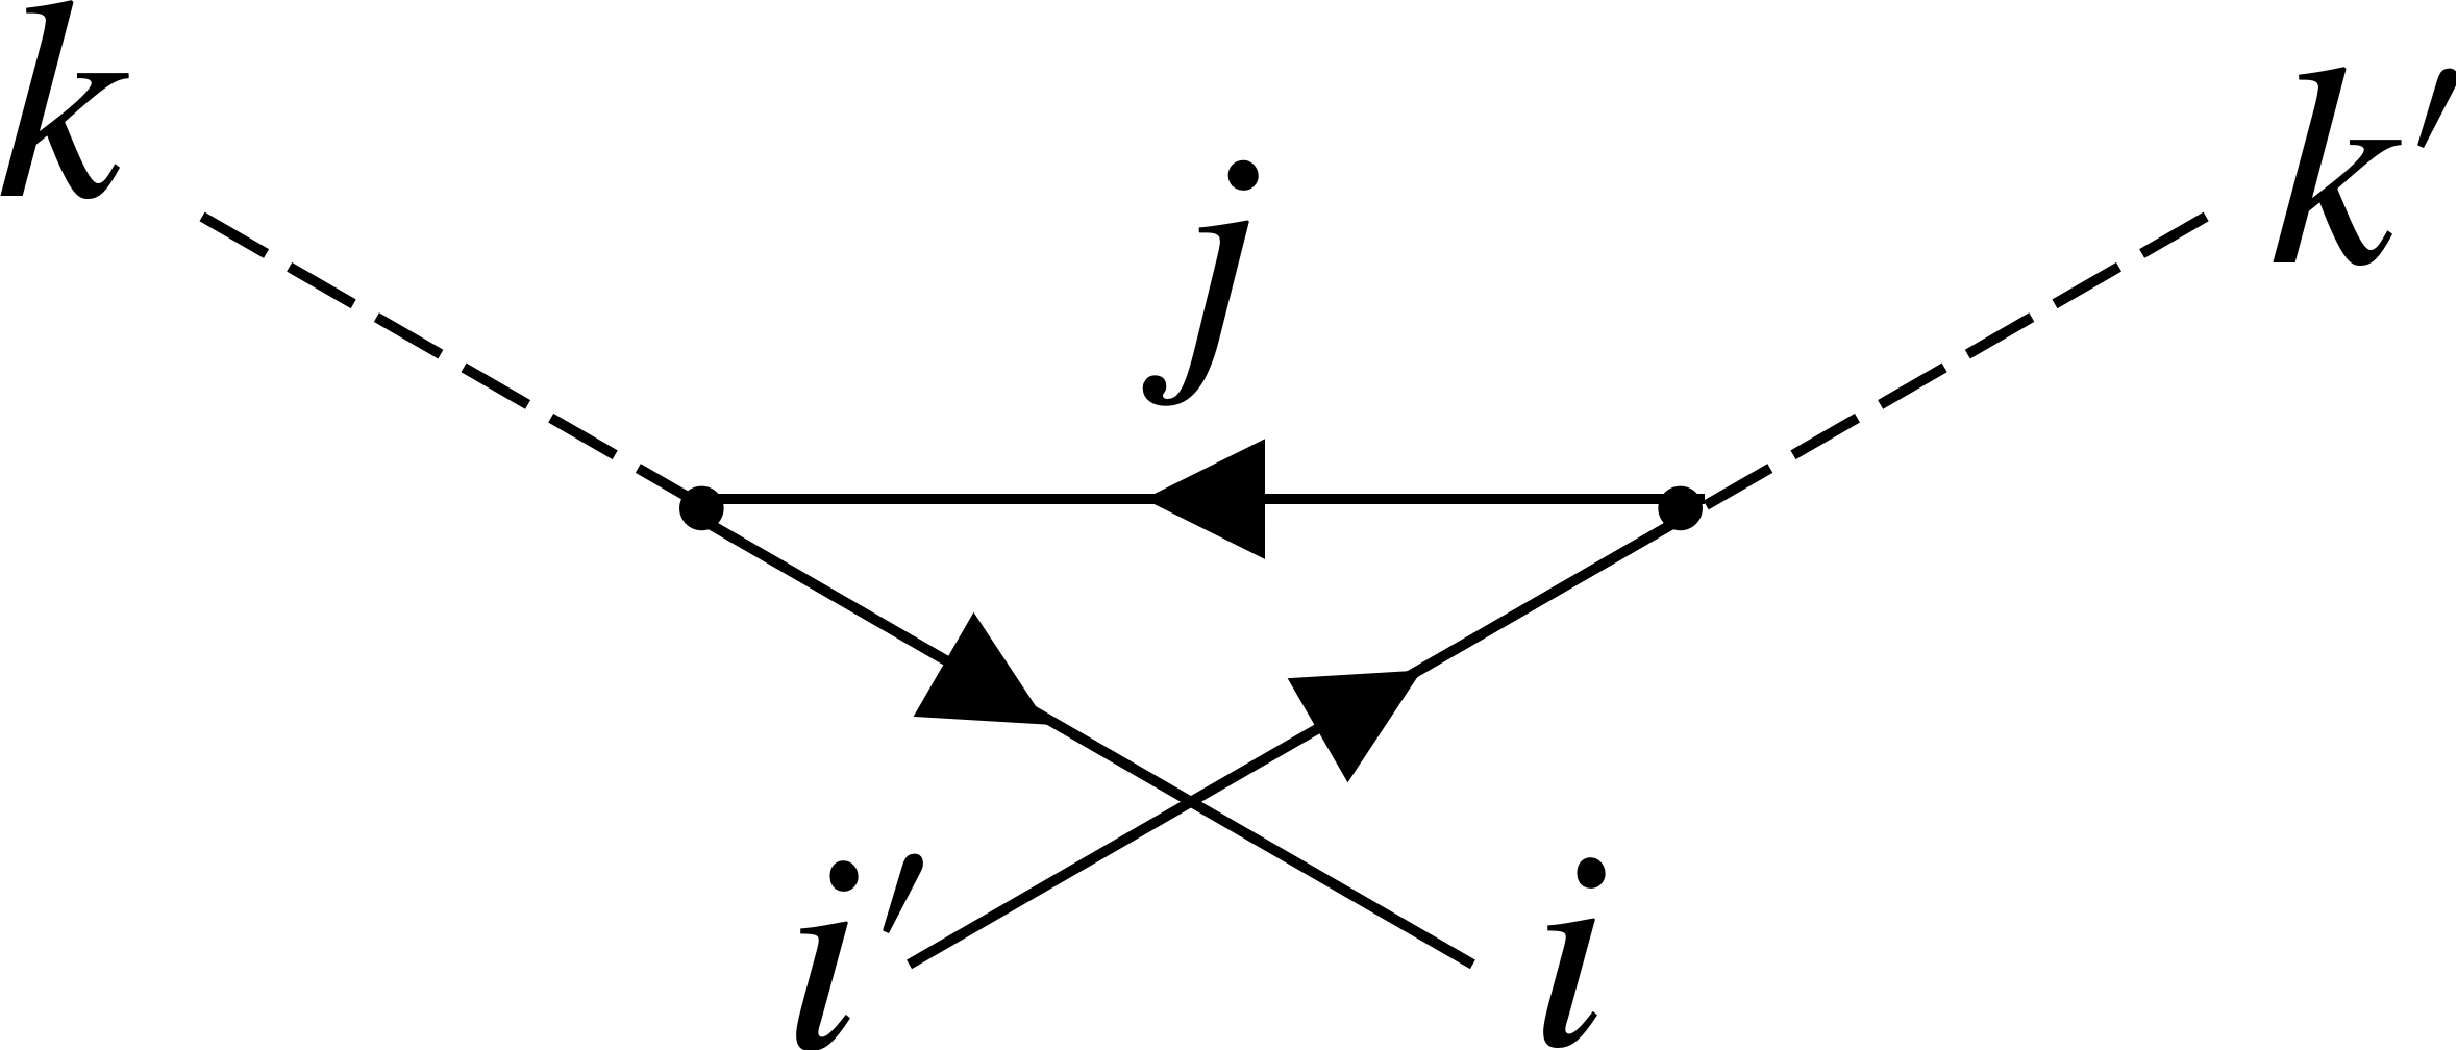
\includegraphics[width=0.15\textwidth]{figures/bfbar-bfbar.pdf} & 
        {\small $\displaystyle 
        \int_{ijki'k'} \frac{(c_k + c_{k'}-c_i - c_{i'}   - 2c_j)  \tilde c_{i'jk'}(0) \tilde c^*_{kij}(0)}
        {(c_{i'} + c_j - c_{k'} )^2 + (c_k- c_{i} - c_{j} )^2 - (c_{i'} + c_{k} - c_{i} - c_{k'})^2}
        \left( e^{- (c_{i'} + c_{k} - c_{i} - c_{k'})^2t} 
        - e^{-\left((c_{i'} + c_j - c_{k'} )^2 + (c_k- c_{i} - c_{j} )^2 \right)t} \right)
        b_{i'}^\dagger b_{i}   a_{k}^\dagger a_{k'}
        $} \\
        \hline
        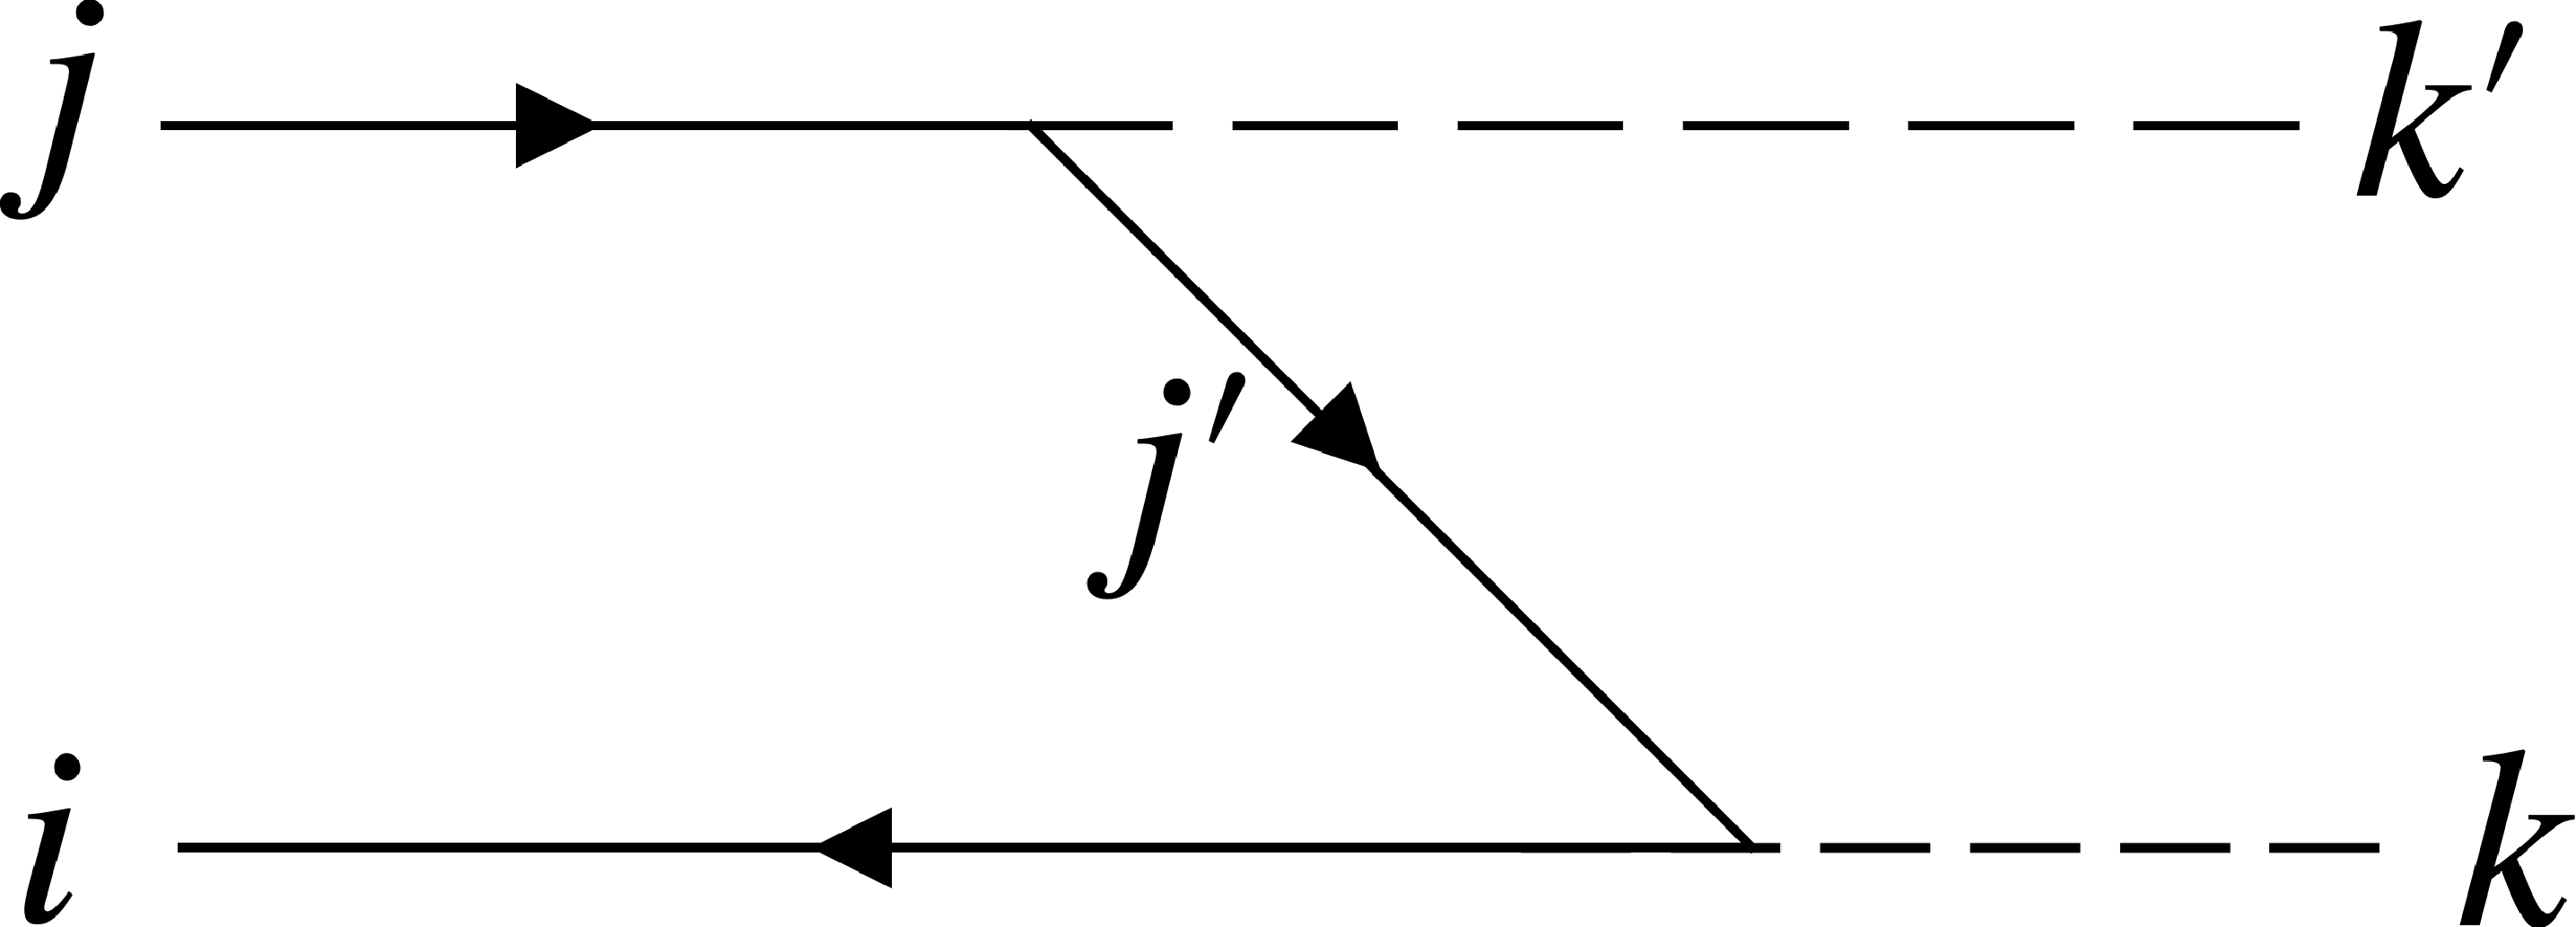
\includegraphics[width=0.15\textwidth]{figures/bb-ffbar(1).pdf} & 
        {\small $\displaystyle 
        \int_{ijki'k'} \frac{(c_j + c_{k}-c_{k'} - c_{i}   - 2c_{j'})  \bar c_{jj'k'}(0) \tilde c_{ij'k}(0)}
        { (c_i - c_{k'} - c_{j'} )^2 + (c_i+ c_{j'} - c_{k} )^2 - (c_i + c_{j} - c_{k'} - c_{k})^2}
        \left( e^{- (c_i + c_{j} - c_{k'} - c_{k})^2t} 
        - e^{-\left( (c_i - c_{k'} - c_{j'} )^2 + (c_i+ c_{j'} - c_{k} )^2 \right)t} \right)
        b_i^\dagger d_{j}^\dagger   a_{k'} a_k
        $} \\
        \hline
        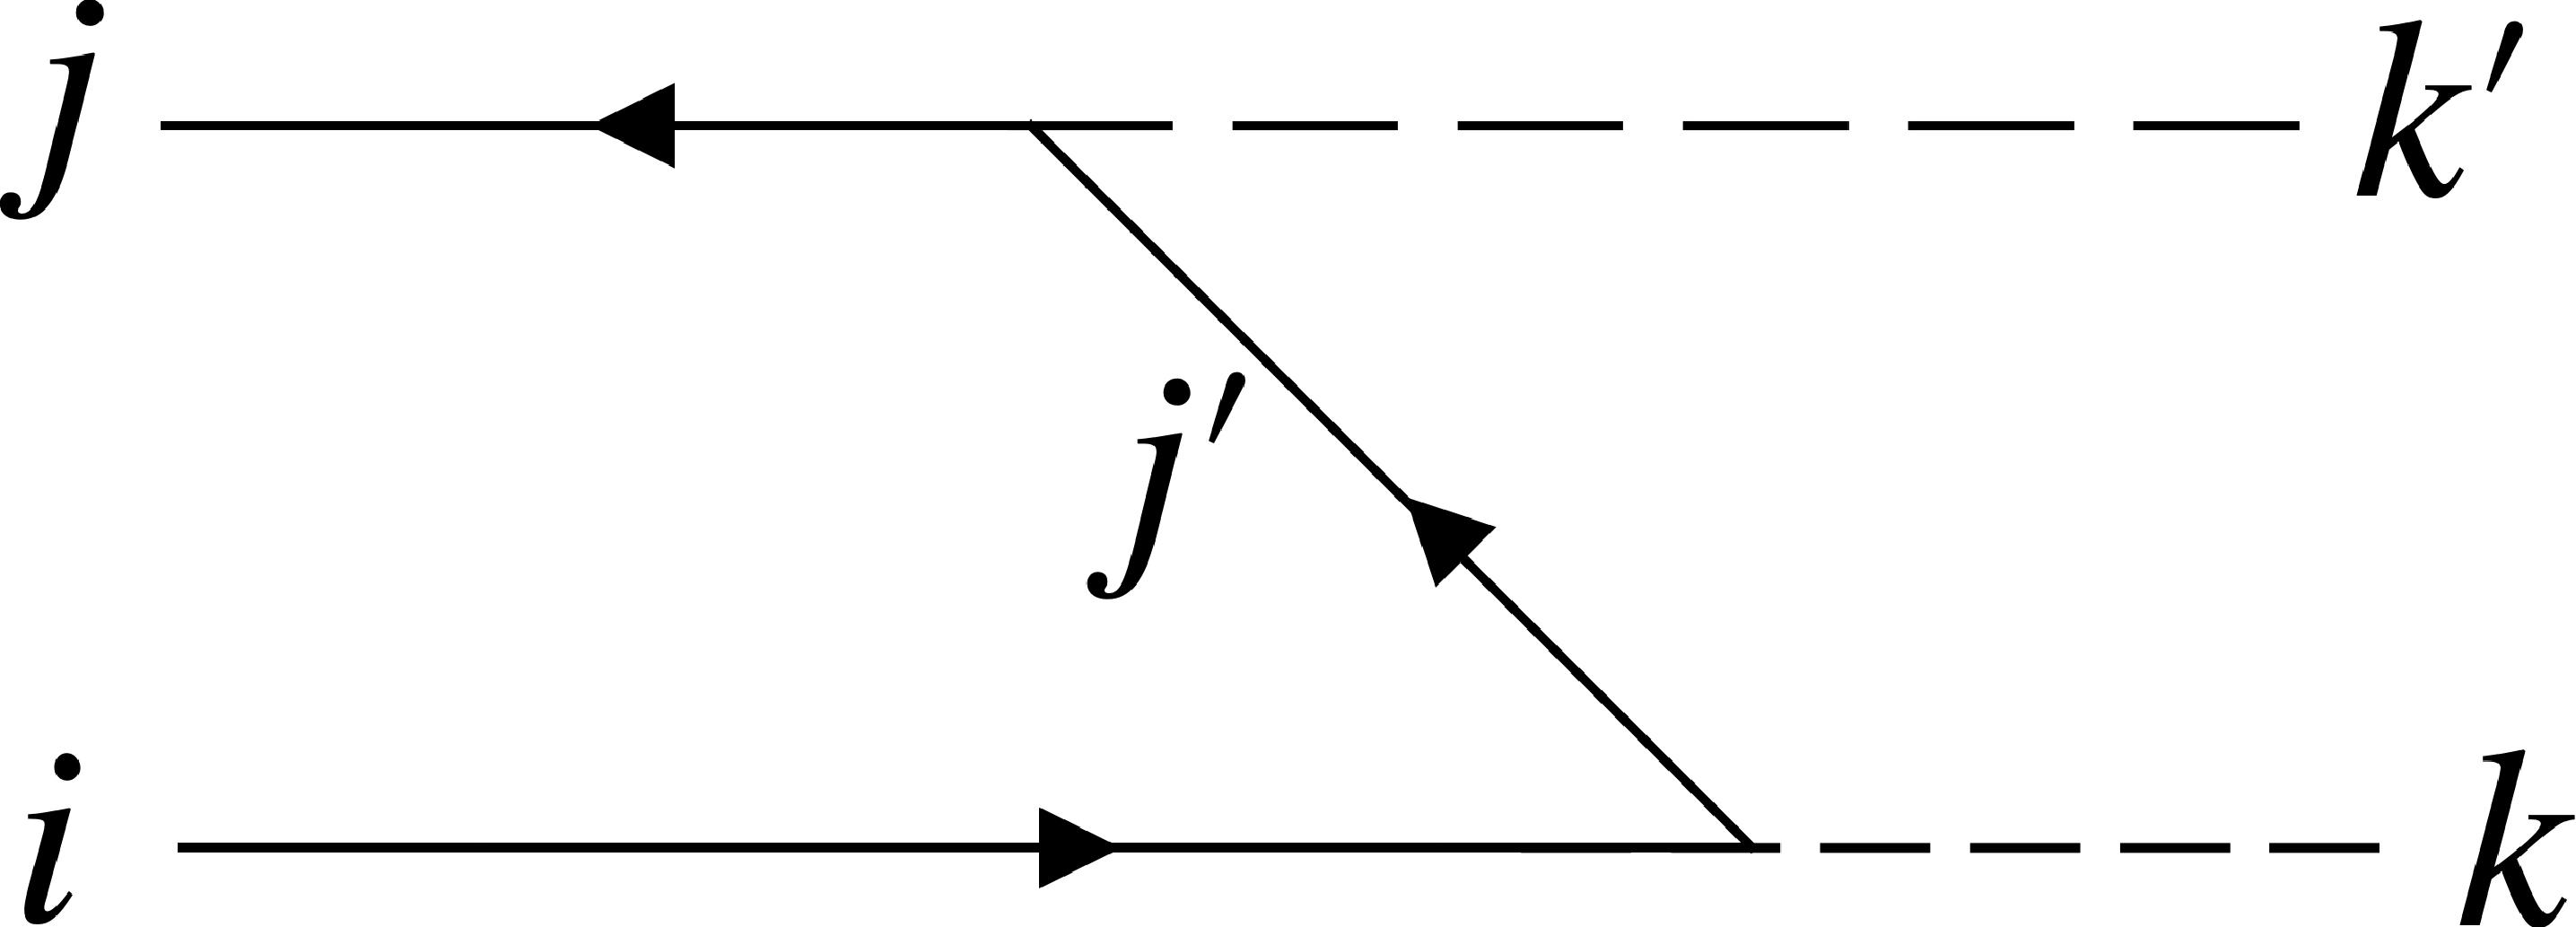
\includegraphics[width=0.15\textwidth]{figures/bb-ffbar(2).pdf} & 
        {\small $\displaystyle 
        \int_{ijki'k'} \frac{(c_j + c_{k}-c_{k'} - c_{i}   - 2c_{j'})  c_{jj'k'}(0) \tilde c_{ij'k}(0)}
        { (c_i - c_{k'} - c_{j'} )^2 + (c_i+ c_{j'} - c_{k} )^2 - (c_i + c_{j} - c_{k'} - c_{k})^2}
        \left( e^{- (c_i + c_{j} - c_{k'} - c_{k})^2t} 
        - e^{-\left( (c_i - c_{k'} - c_{j'} )^2 + (c_i+ c_{j'} - c_{k} )^2 \right)t} \right)
        b_j^\dagger d_{i}^\dagger   a_{k'} a_k
        $} \\
        \hline
        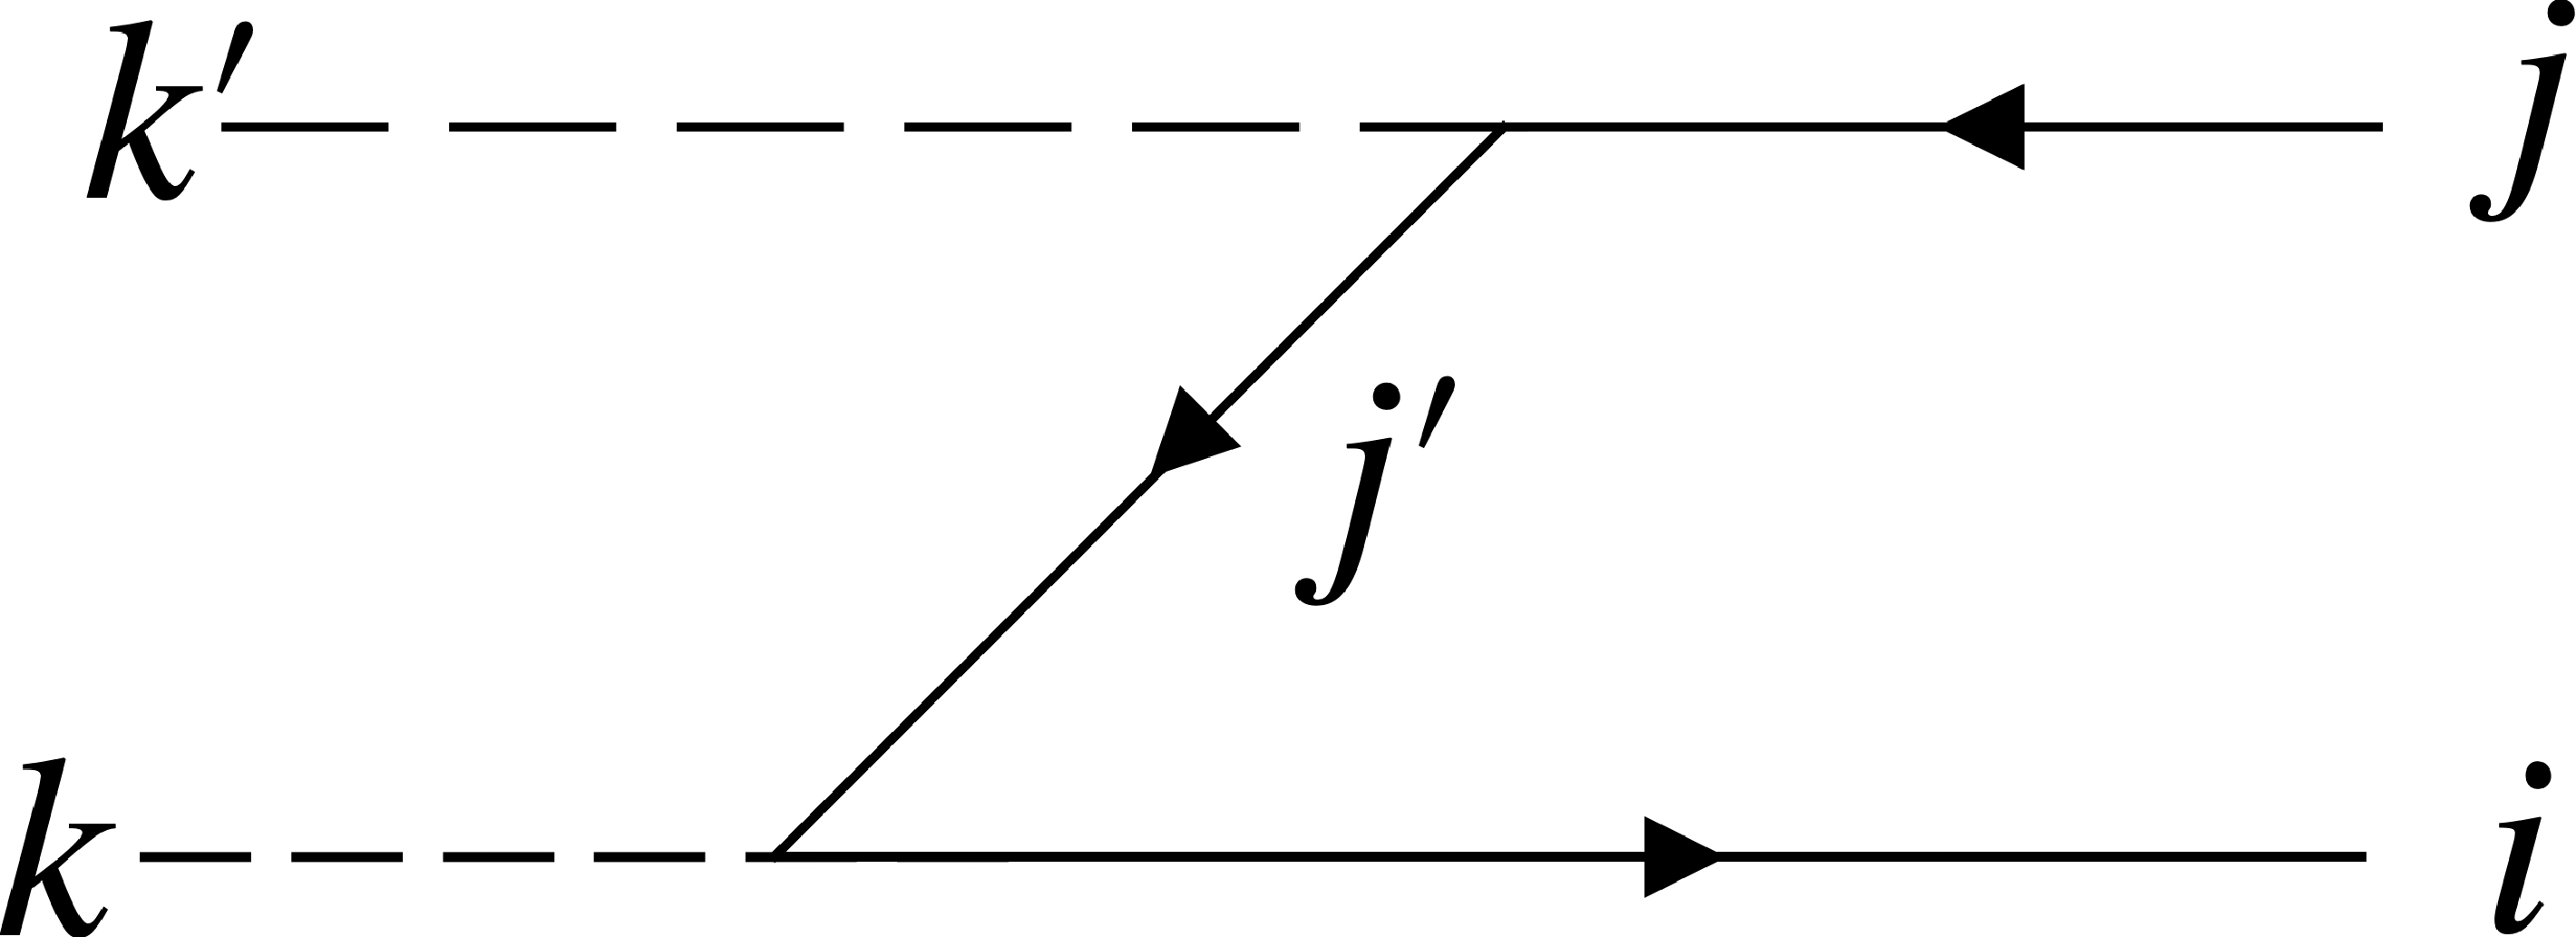
\includegraphics[width=0.15\textwidth]{figures/ffbar-bb(1).pdf} & 
        {\small $\displaystyle 
        \int_{ijki'k'} \frac{(c_j + c_{k}-c_{k'} - c_{i}   - 2c_{j'})  c^*_{jj'k'}(0) \tilde c^*_{ij'k}(0)}
        { (c_{k'} + c_{j'} - c_{j} )^2 + (c_k- c_{j'} - c_{i} )^2 -(c_k + c_{k'} - c_{i'} - c_{j})^2}
        \left( e^{- (c_k + c_{k'} - c_{i'} - c_{j})^2t} 
        - e^{-\left((c_{k'} + c_{j'} - c_{j} )^2 + (c_k- c_{j'} - c_{i} )^2 \right)t} \right)
        b_j d_{i}   a_{k'}^\dagger a_k ^\dagger
        $} \\
        \hline
        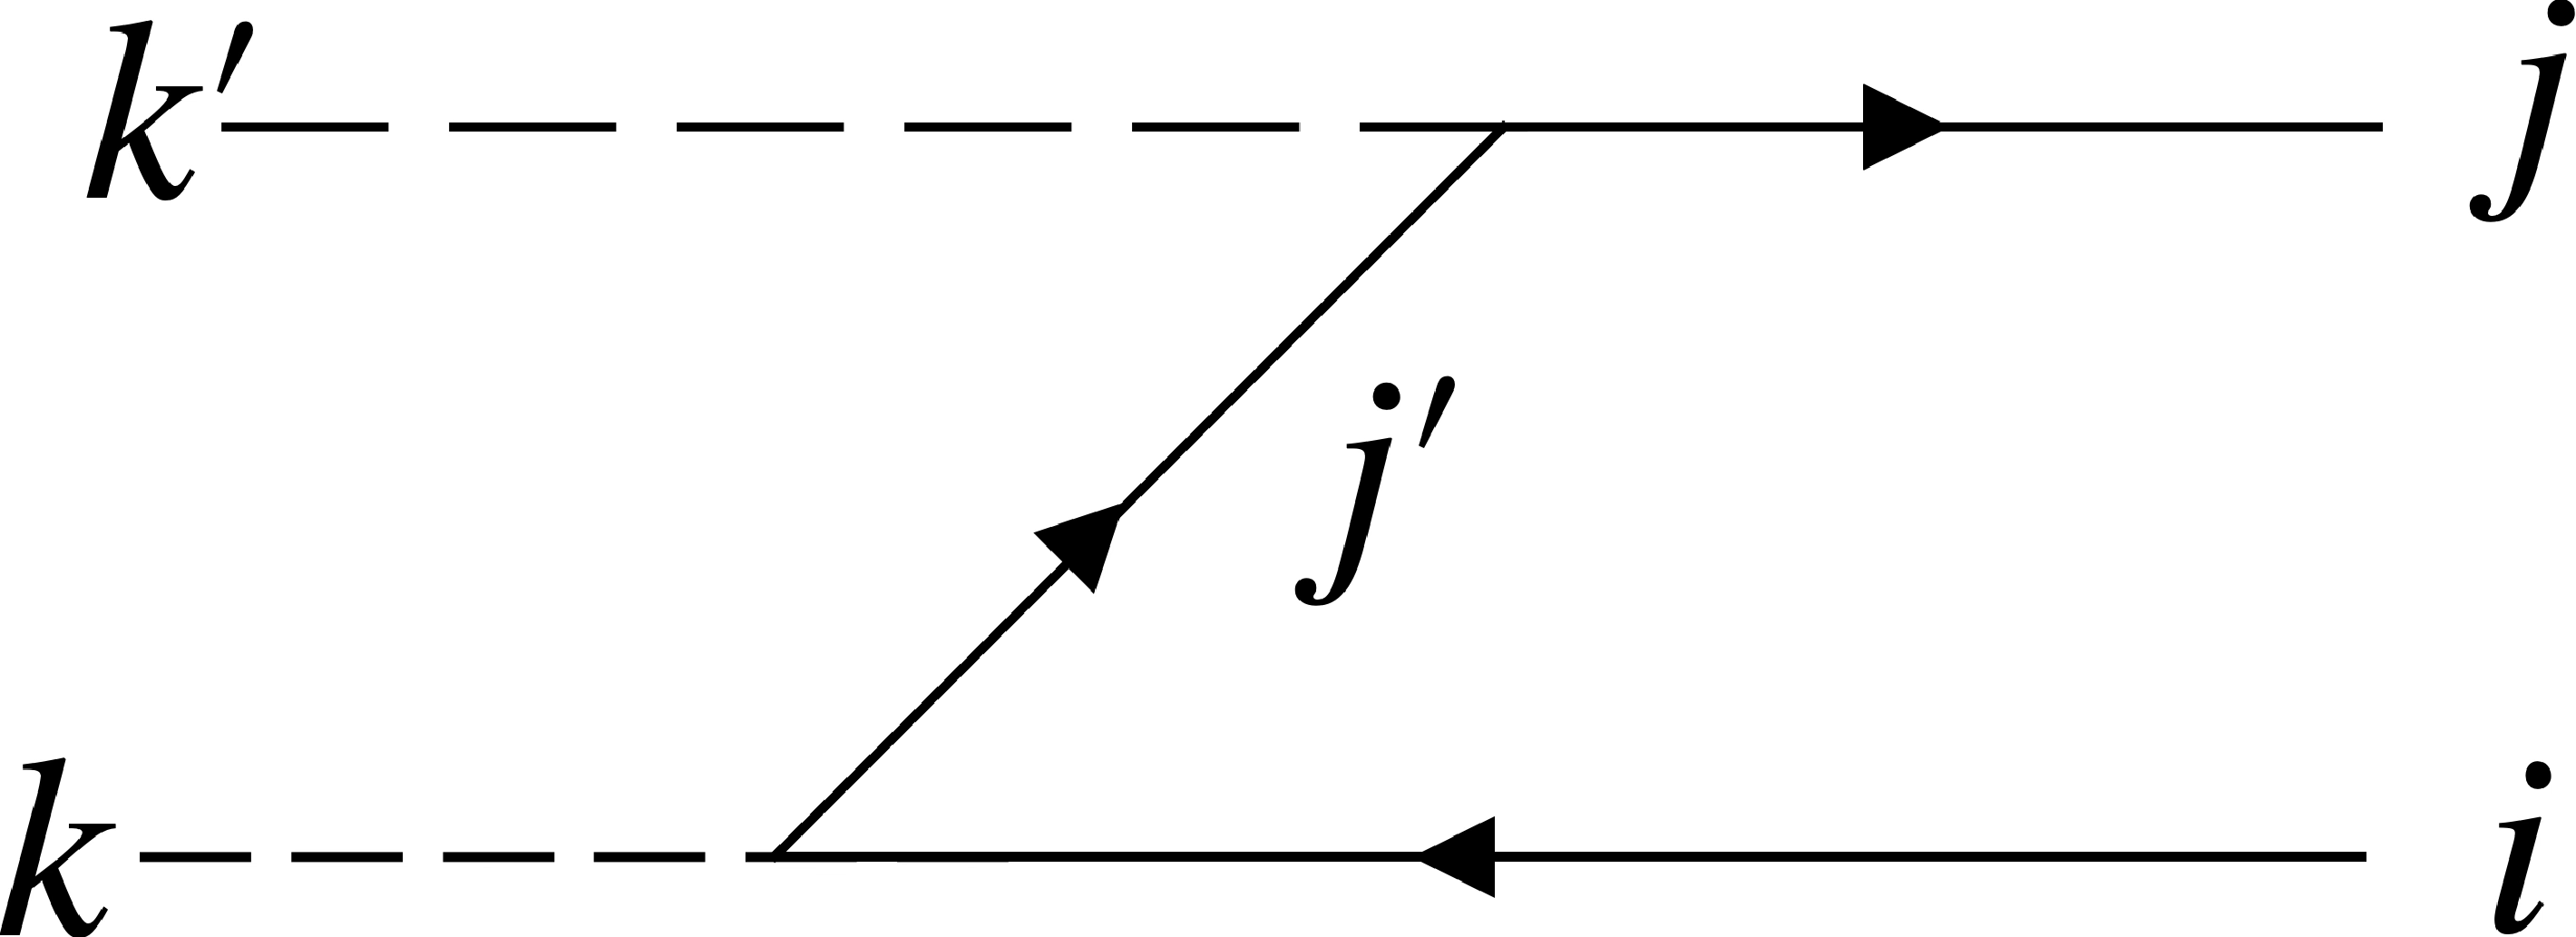
\includegraphics[width=0.15\textwidth]{figures/ffbar-bb(2).pdf} & 
        {\small $\displaystyle 
        \int_{ijki'k'} \frac{(c_j + c_{k}-c_{k'} - c_{i}   - 2c_{j'})  \bar c^*_{jj'k'}(0) \tilde c^*_{ij'k}(0)}
        { (c_{k'} + c_{j'} - c_{j} )^2 + (c_k- c_{j'} - c_{i} )^2 -(c_k + c_{k'} - c_{i'} - c_{j})^2}
        \left( e^{- (c_k + c_{k'} - c_{i'} - c_{j})^2t} 
        - e^{-\left((c_{k'} + c_{j'} - c_{j} )^2 + (c_k- c_{j'} - c_{i} )^2 \right)t} \right)
        b_i d_{j}   a_{k'}^\dagger a_k^\dagger
        $} \\
        \hline
    \end{tabular}
    
\end{table}


\begin{table}[h]
    \centering
    \hspace*{-1.7cm} % Move table to the left
    \begin{tabular}{|c|c|}
        \hline
        %1-3 or 3-1 diagrams
        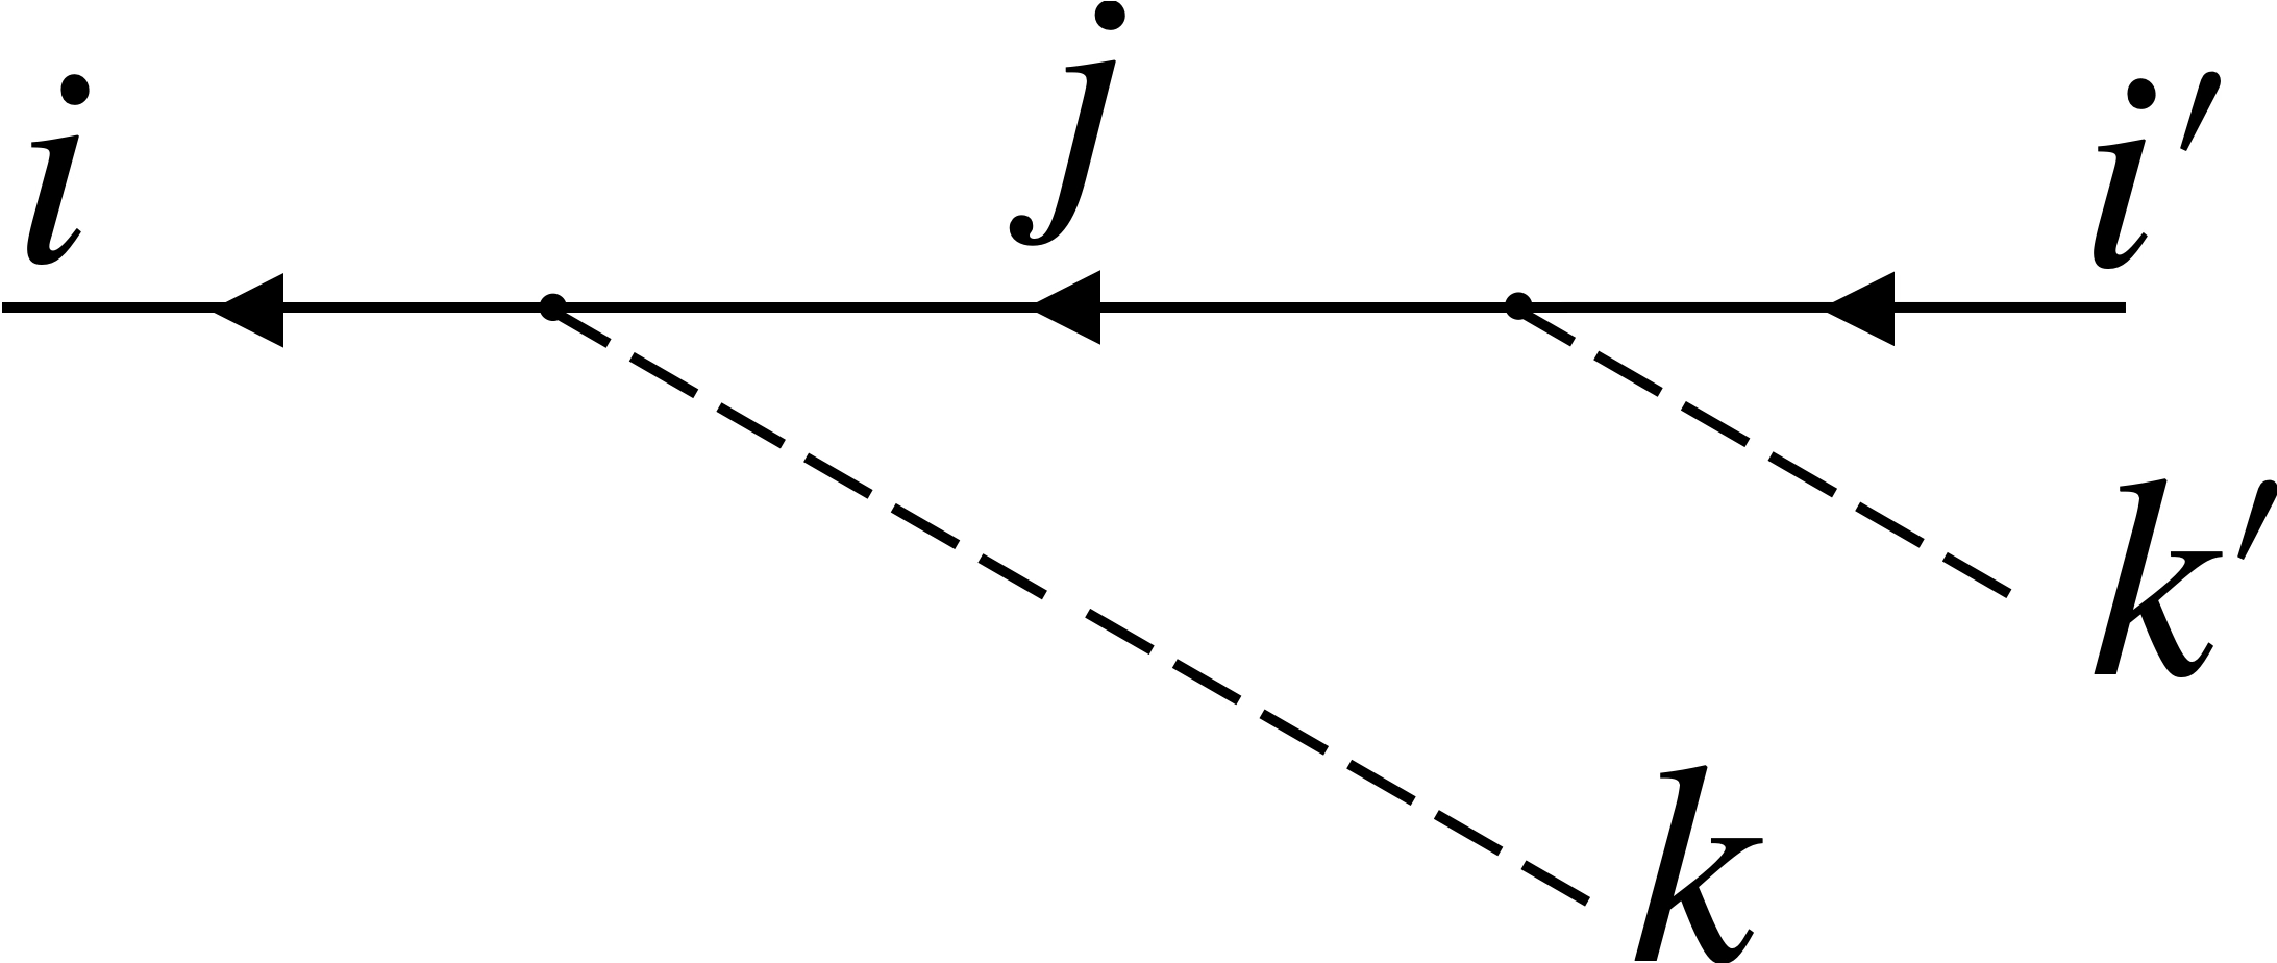
\includegraphics[width=0.15\textwidth]{figures/fbb-f.pdf} & 
        {\small $\displaystyle 
        \int_{ijki'k'} \frac{(c_i + c_{k'} + c_{i'} - c_k - 2c_j)  c_{ijk}(0)  c_{ji'k'}(0)}
        { (c_i - c_j - c_k)^2 + (c_j - c_{i'} - c_{j'})^2 -(c_i - c_k - c_{i'} - c_{k'})^2}
        \left( e^{- (c_i - c_k - c_{i'} - c_{k'})^2t} 
        - e^{-\left((c_i - c_j - c_k)^2 + (c_j - c_{i'} - c_{j'})^2 \right)t} \right)
        b_i^\dagger b_{i'}   a_{k'} a_k
        $} \\
        \hline
        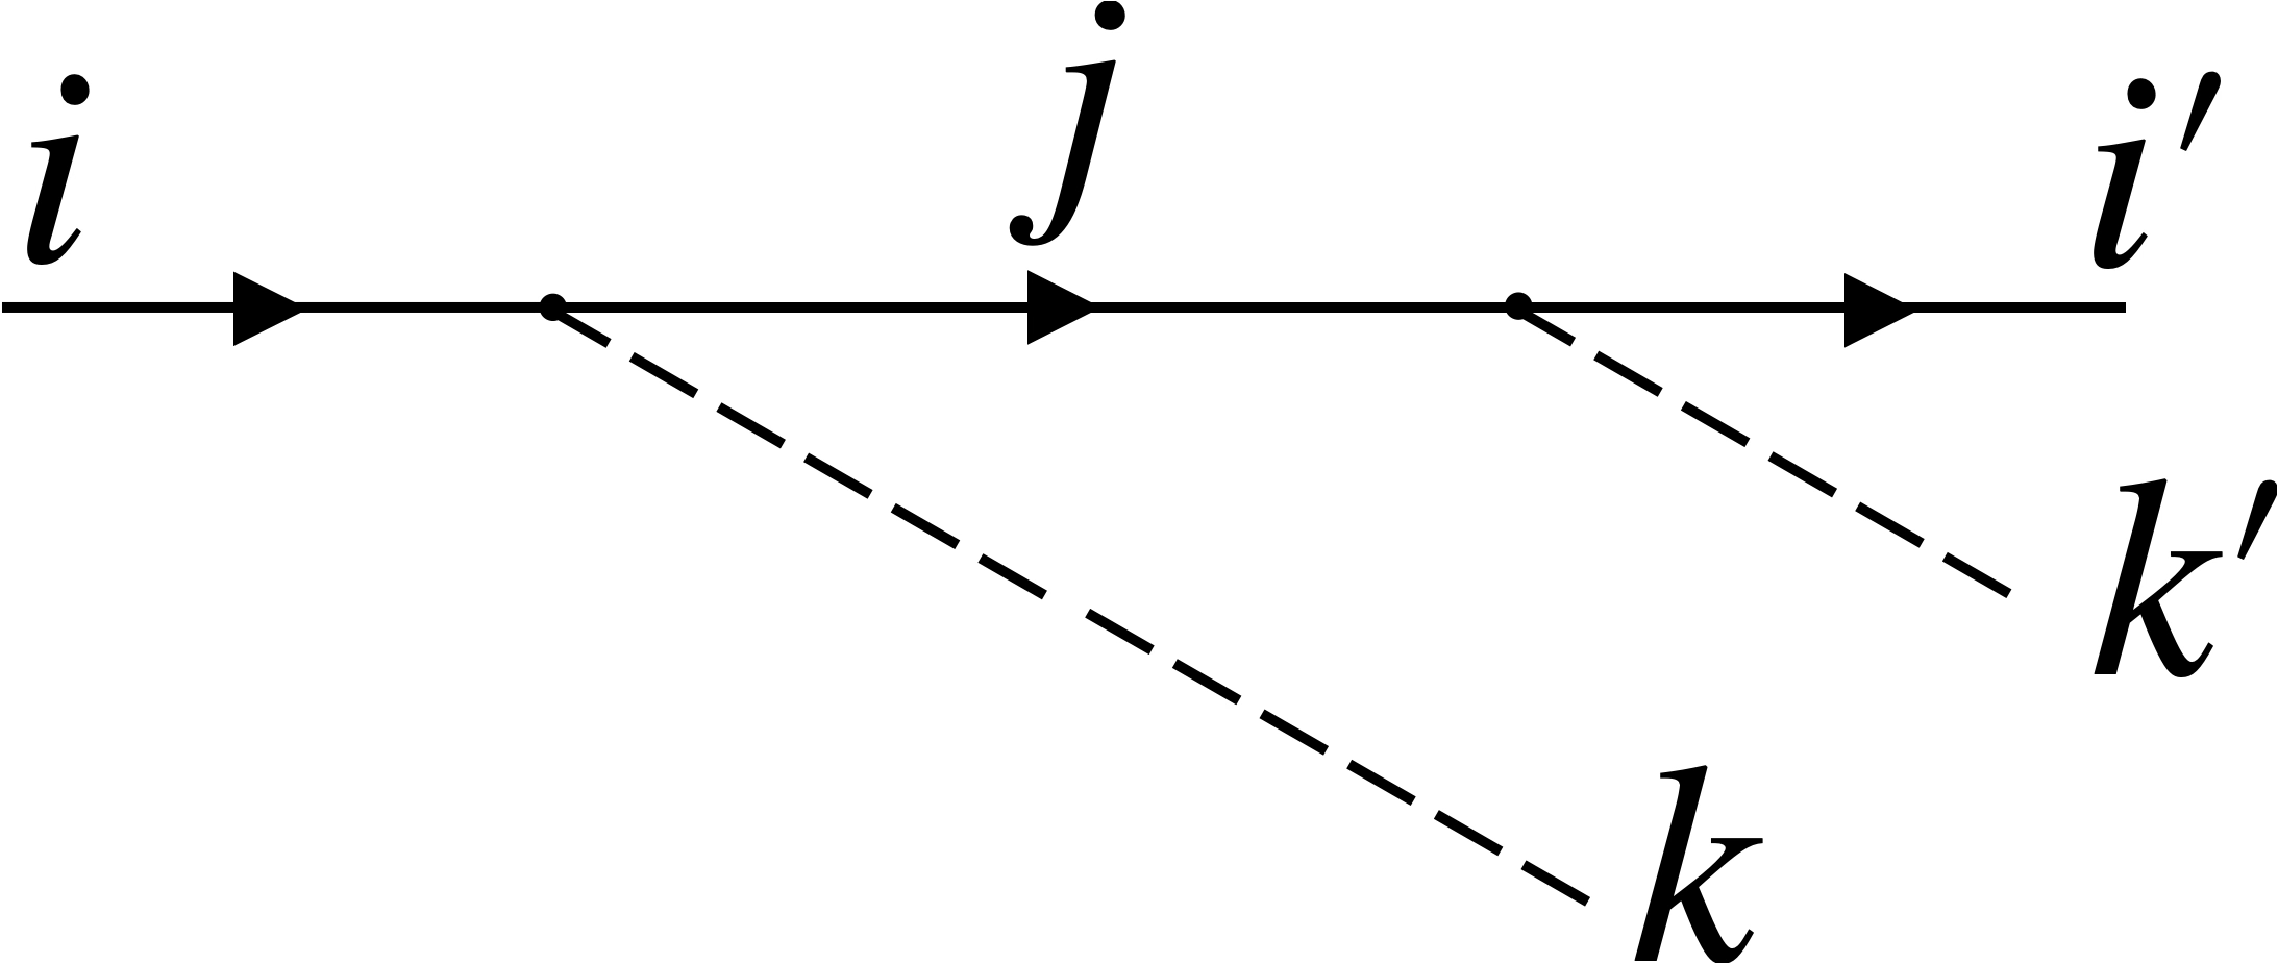
\includegraphics[width=0.15\textwidth]{figures/fbarbb-fbar.pdf} & 
        {\small $\displaystyle 
        \int_{ijki'k'} \frac{(c_i + c_{k'} + c_{i'} - c_k - 2c_j)  \bar c_{ijk}(0)  \bar c_{ji'k'}(0)}
        { (c_i - c_j - c_k)^2 + (c_j - c_{i'} - c_{j'})^2 -(c_i - c_k - c_{i'} - c_{k'})^2}
        \left( e^{- (c_i - c_k - c_{i'} - c_{k'})^2t} 
        - e^{-\left((c_i - c_j - c_k)^2 + (c_j - c_{i'} - c_{j'})^2 \right)t} \right)
        d_i^\dagger d_{i'}   a_{k'} a_k
        $} \\
        \hline
        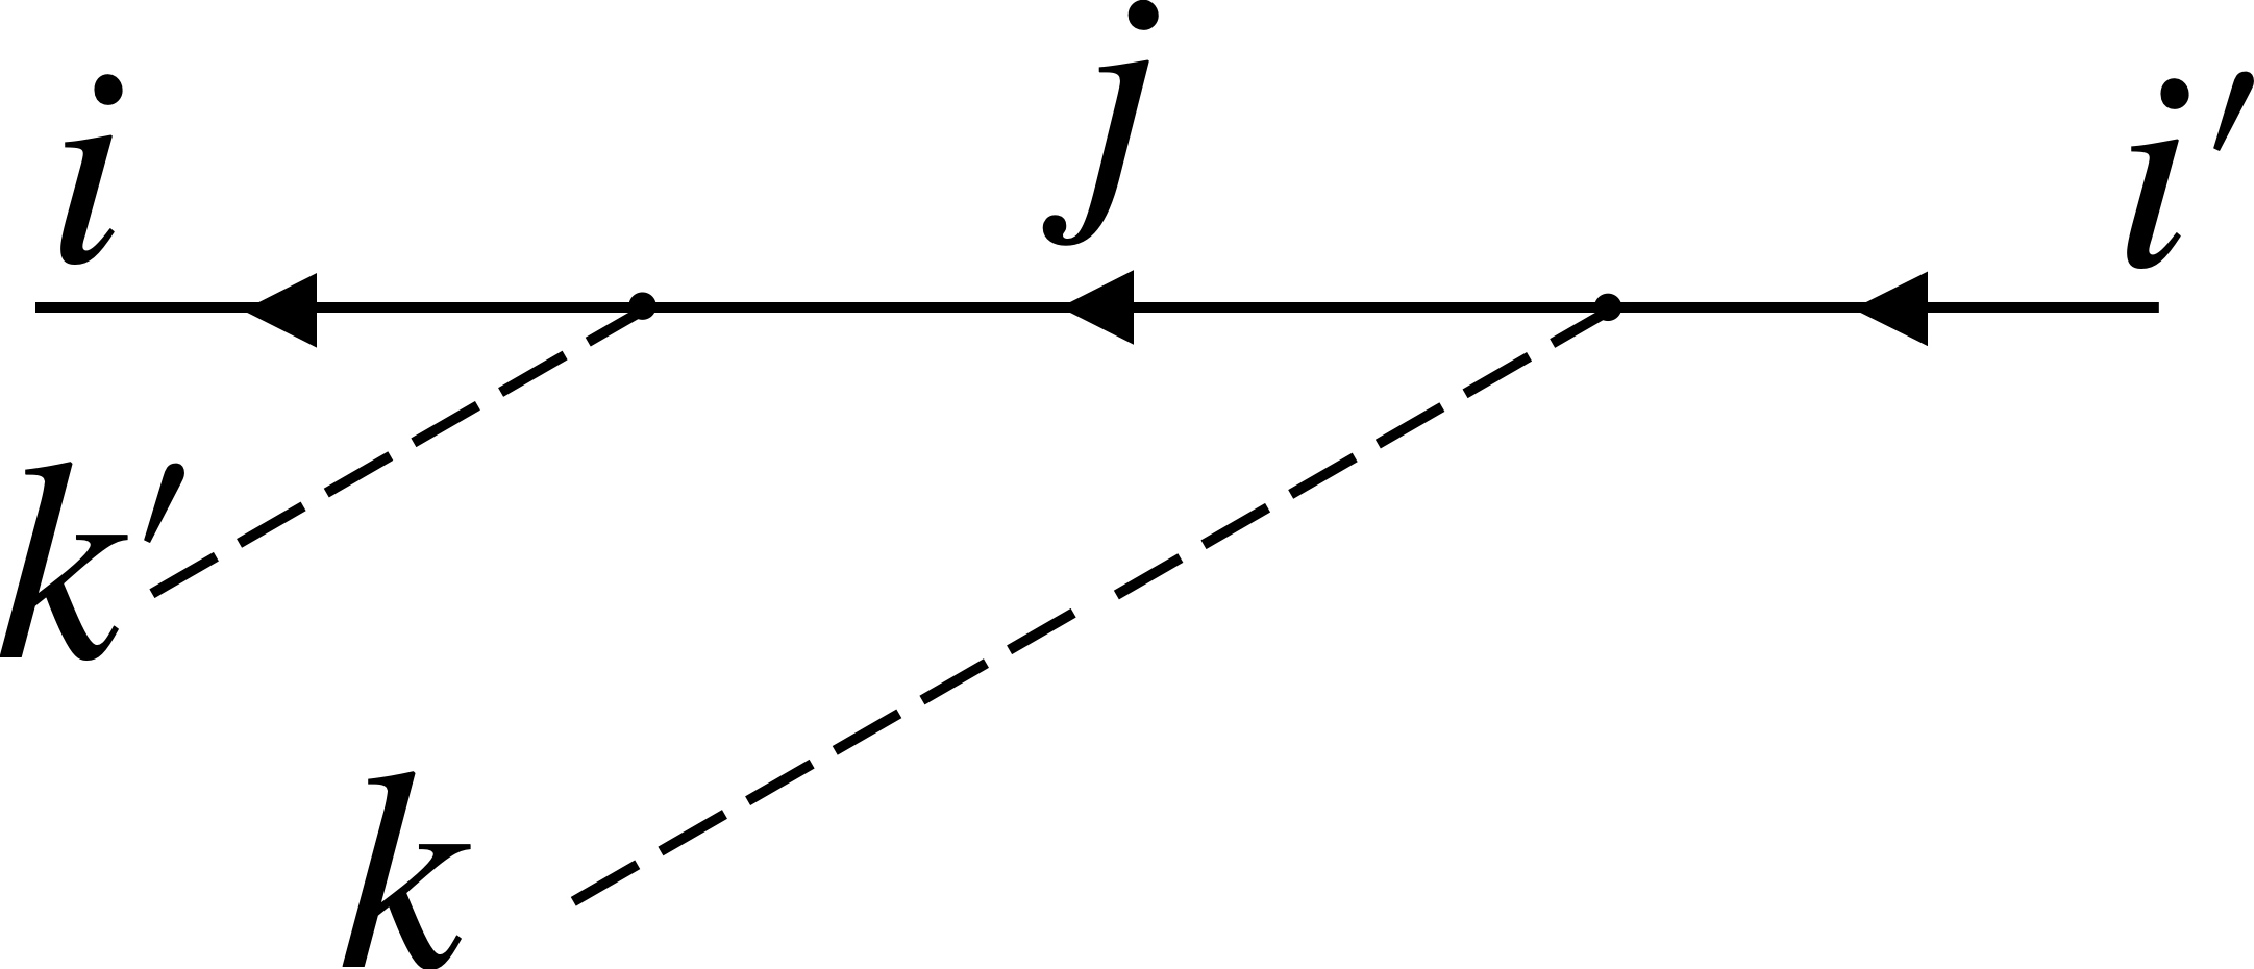
\includegraphics[width=0.15\textwidth]{figures/f-fbb.pdf} & 
        {\small $\displaystyle 
        \int_{ijki'k'} \frac{(c_i + c_{k'} + c_{i'} - c_k - 2c_j)   c^*_{ik'j}(0)  c^*_{jki'}(0)}
        { (c_i + c_{k'} - c_j )^2 + (c_j + c_{k} - c_{i'})^2 -(c_i + c_k + c_{k'} - c_{i'})^2}
        \left( e^{-(c_i + c_k + c_{k'} - c_{i'})^2t} 
        - e^{-\left((c_i + c_{k'} - c_j )^2 + (c_j + c_{k} - c_{i'})^2 \right)t} \right)
        b_i^\dagger b_{i'}   a_{k'}^\dagger a_k^\dagger
        $} \\
        \hline
        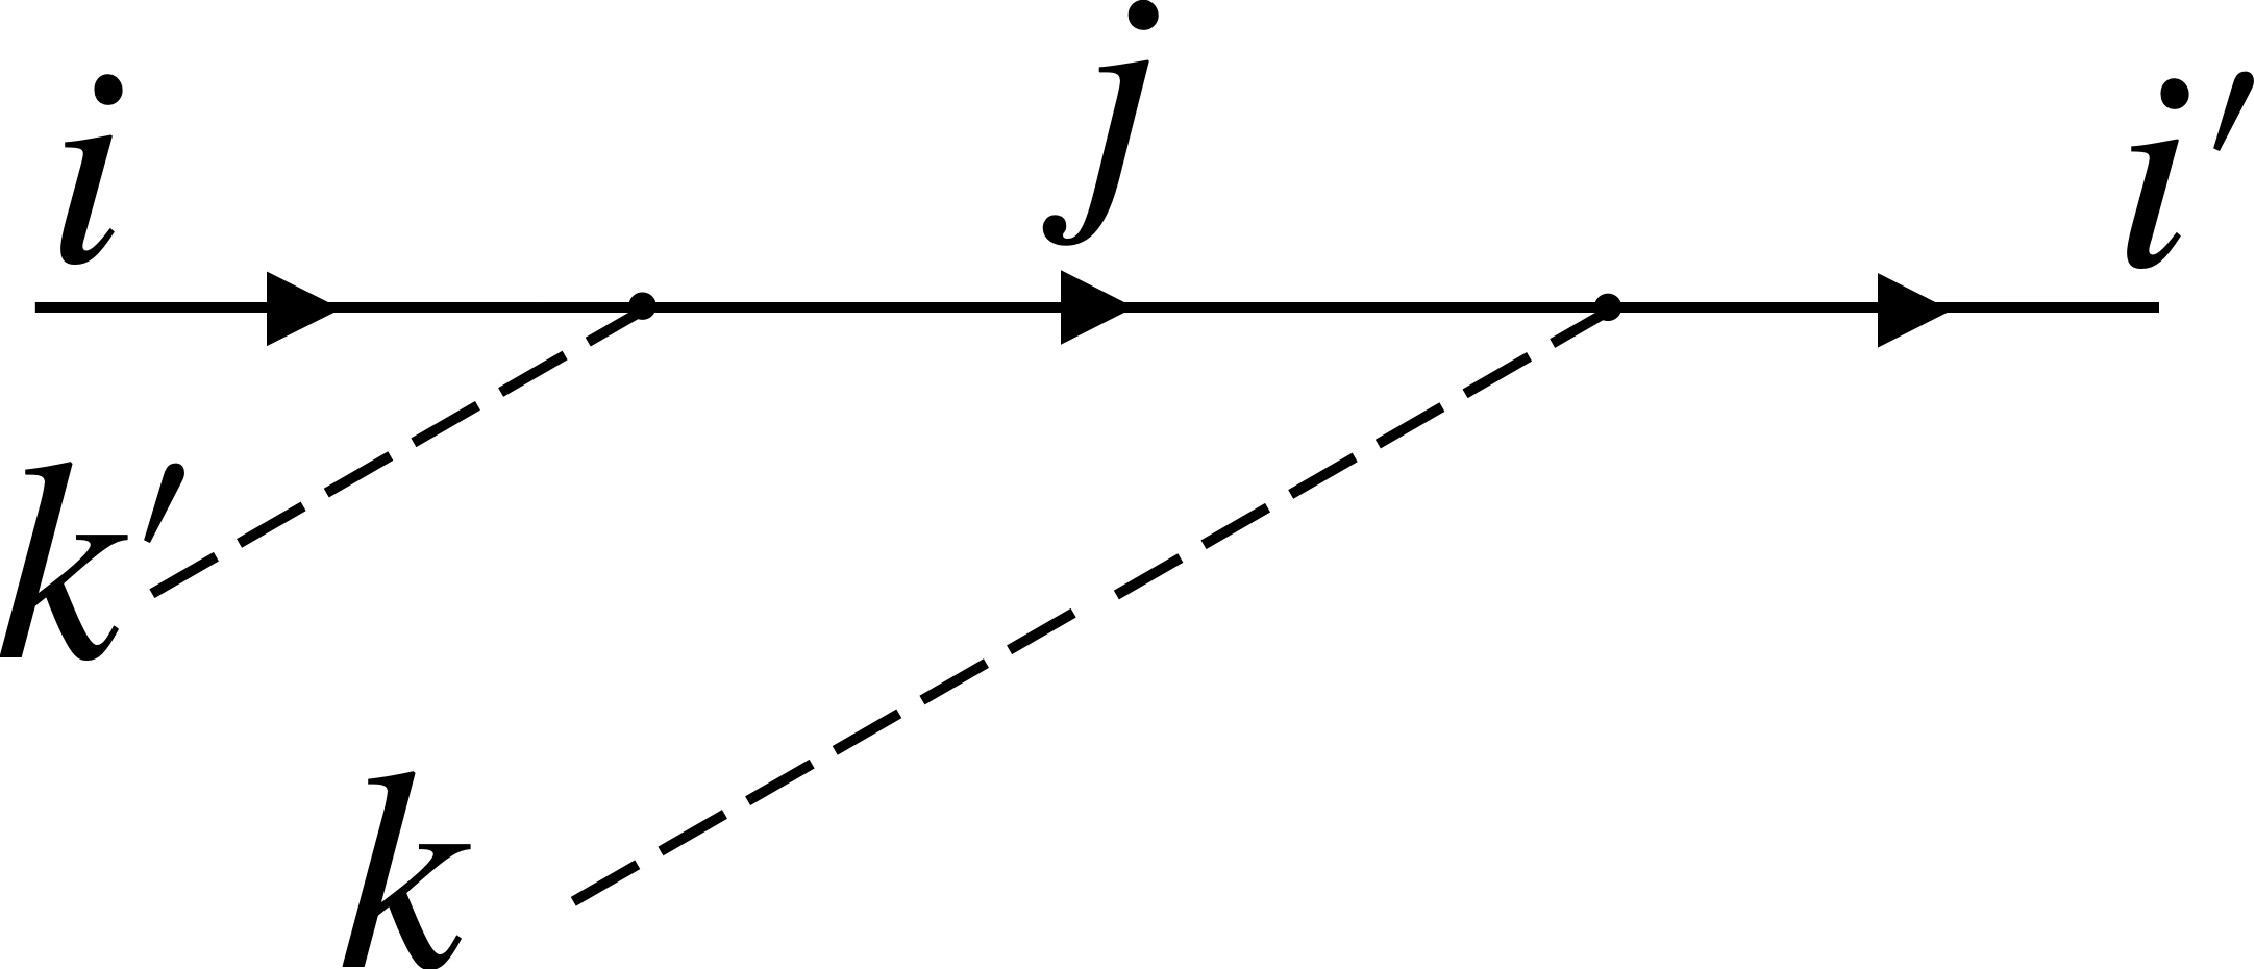
\includegraphics[width=0.15\textwidth]{figures/fbar-fbarbb.pdf} & 
        {\small $\displaystyle 
        \int_{ijki'k'} \frac{(c_i + c_{k'} + c_{i'} - c_k - 2c_j)   \bar c^*_{ik'j}(0)  \bar c^*_{jki'}(0)}
        { (c_i + c_{k'} - c_j )^2 + (c_j + c_{k} - c_{i'})^2 -(c_i + c_k + c_{k'} - c_{i'})^2}
        \left( e^{-(c_i + c_k + c_{k'} - c_{i'})^2t} 
        - e^{-\left((c_i + c_{k'} - c_j )^2 + (c_j + c_{k} - c_{i'})^2 \right)t} \right)
        d_i^\dagger d_{i'}   a_{k'}^\dagger a_k^\dagger
        $} \\
        \hline
        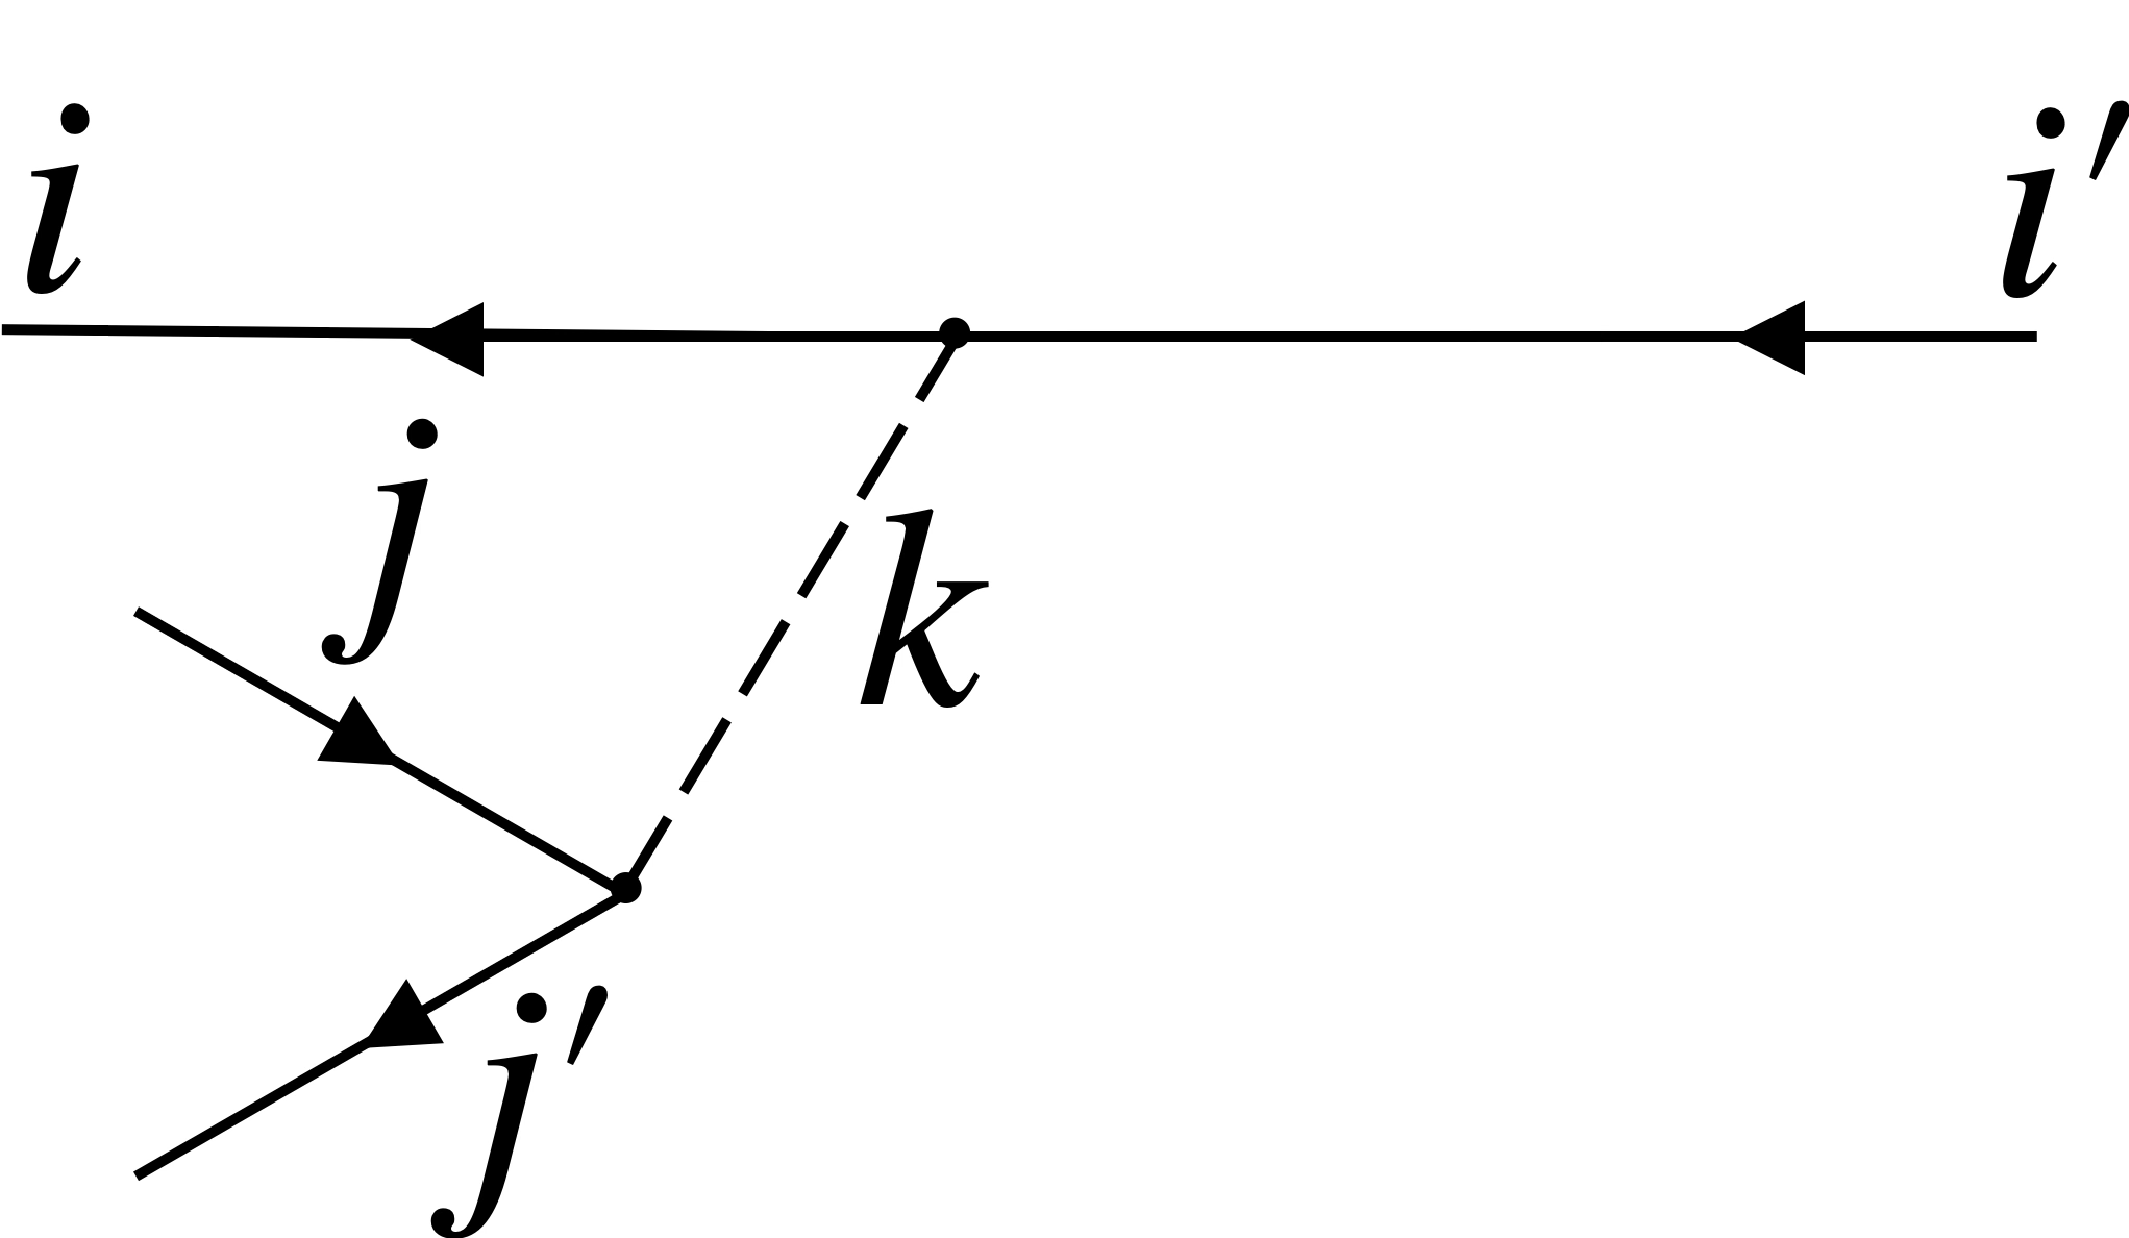
\includegraphics[width=0.15\textwidth]{figures/f-fffbar.pdf} & 
        {\small $\displaystyle 
        \int_{ijki'k'} \frac{(c_{i'} + c_{j} + c_{j'} - c_i - 2c_k)   c^*_{iki'}(0)  \tilde c_{ij'k}(0)}
        { (c_i + c_k - c_{i'})^2 + (c_i + c_{j'} - c_k)^2 -(c_i + c_j + c_{j'} - c_{i'})^2}
        \left( e^{-(c_i + c_j + c_{j'} - c_{i'})^2t} 
        - e^{-\left( (c_i + c_k - c_{i'})^2 + (c_i + c_{j'} - c_k)^2 \right)t} \right)
        b_i^\dagger b_{j'}^\dagger  b_{i'}  d_{j}^\dagger 
        $} \\
        \hline
        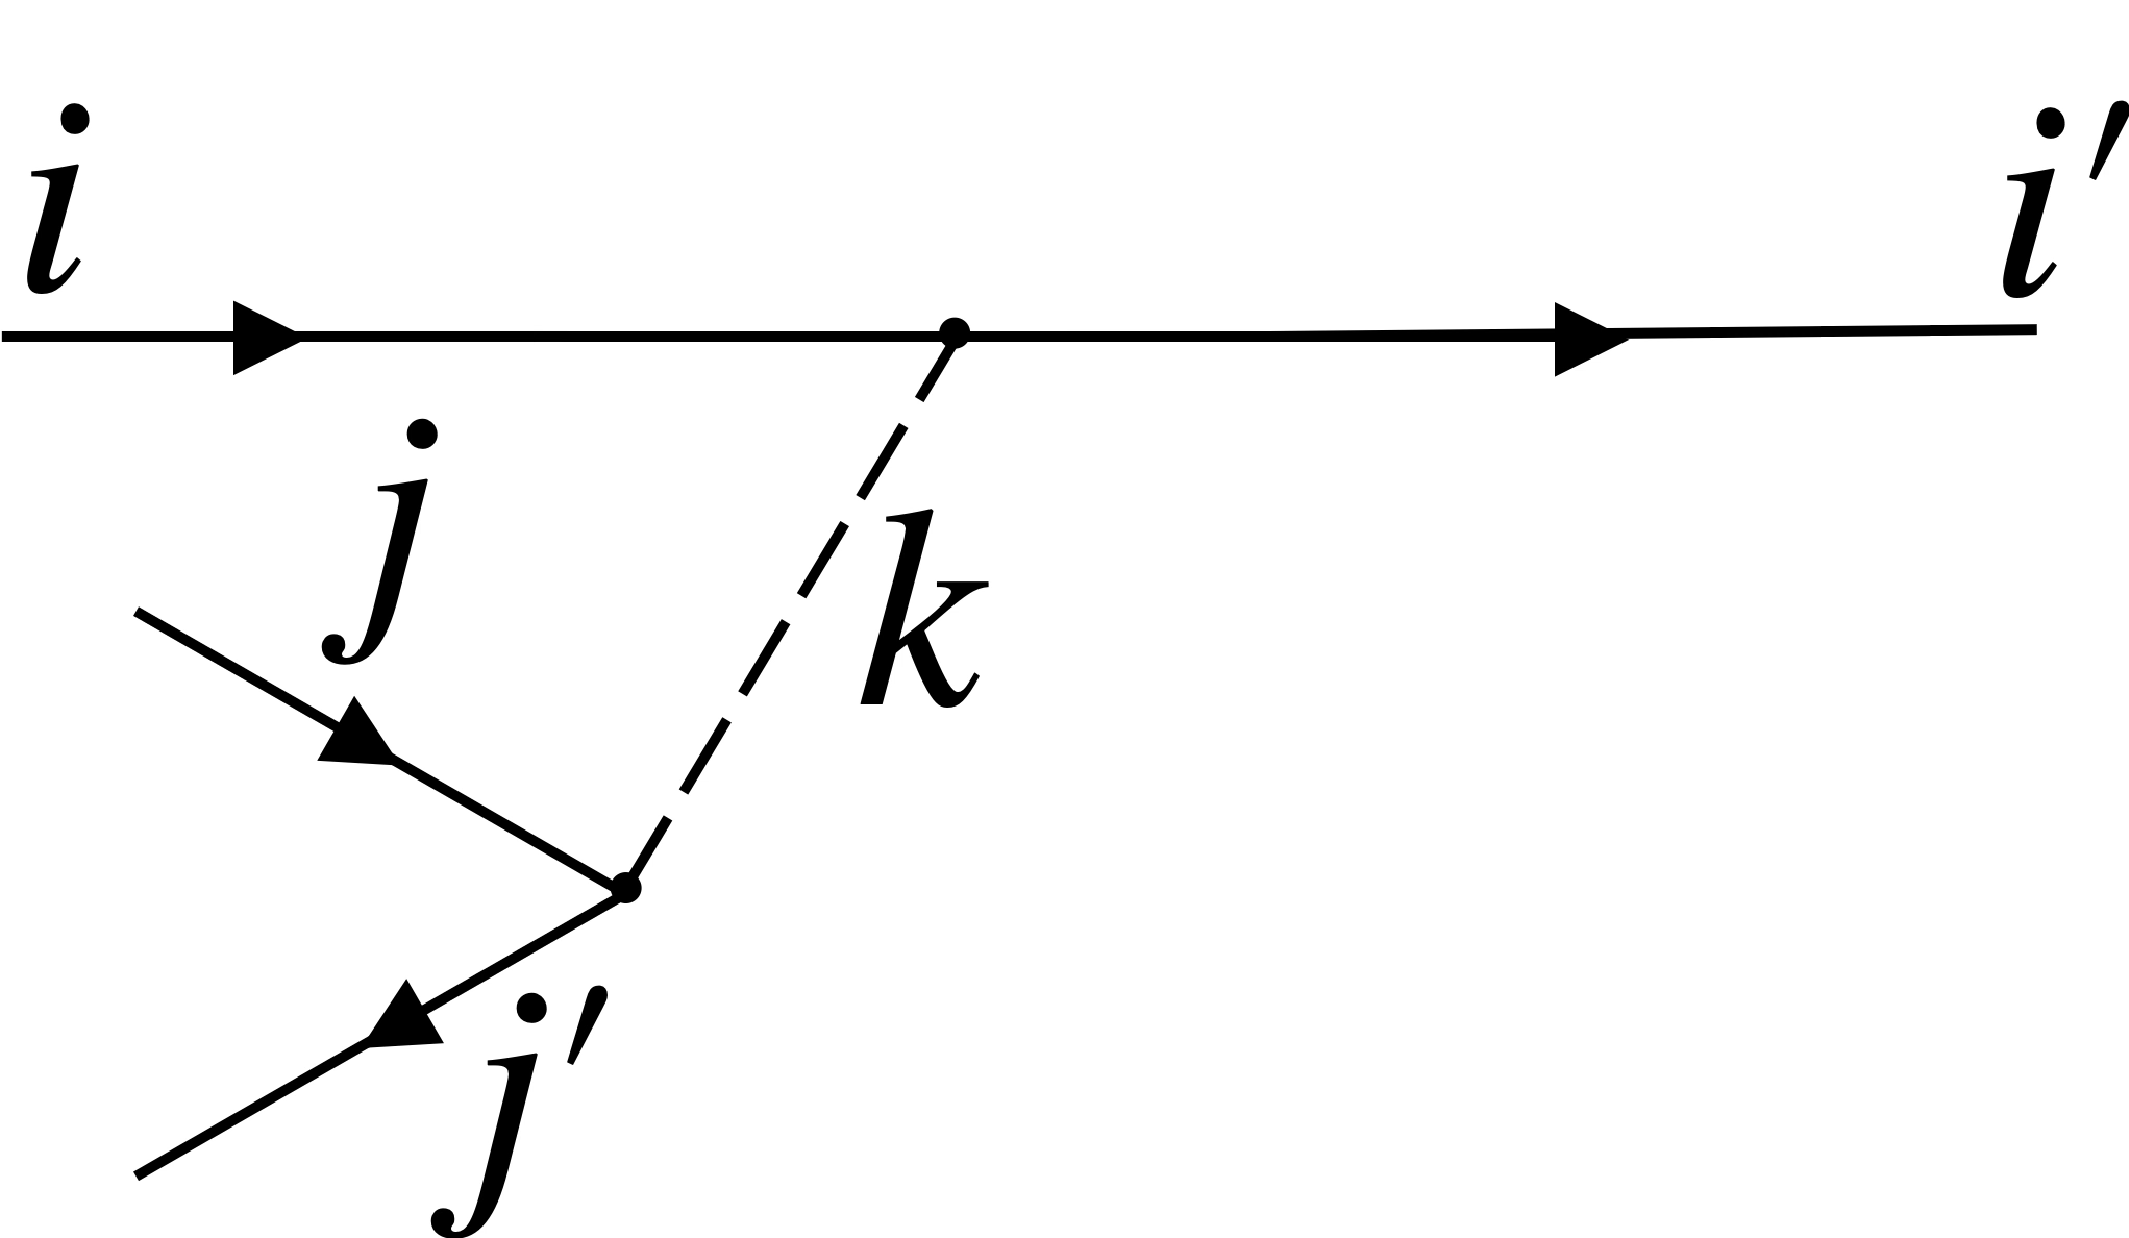
\includegraphics[width=0.15\textwidth]{figures/fbar-ffbarfbar.pdf} & 
        {\small $\displaystyle 
        \int_{ijki'k'} \frac{(c_{i'} + c_{j} + c_{j'} - c_i - 2c_k)   \bar c^*_{iki'}(0)  \tilde c_{ij'k}(0)}
        { (c_i + c_k - c_{i'})^2 + (c_i + c_{j'} - c_k)^2 -(c_i + c_j + c_{j'} - c_{i'})^2}
        \left( e^{-(c_i + c_j + c_{j'} - c_{i'})^2t} 
        - e^{-\left( (c_i + c_k - c_{i'})^2 + (c_i + c_{j'} - c_k)^2 \right)t} \right)
        b_{j'}^\dagger d_i^\dagger d_{j}^\dagger d_{i'}
        $} \\
        \hline
        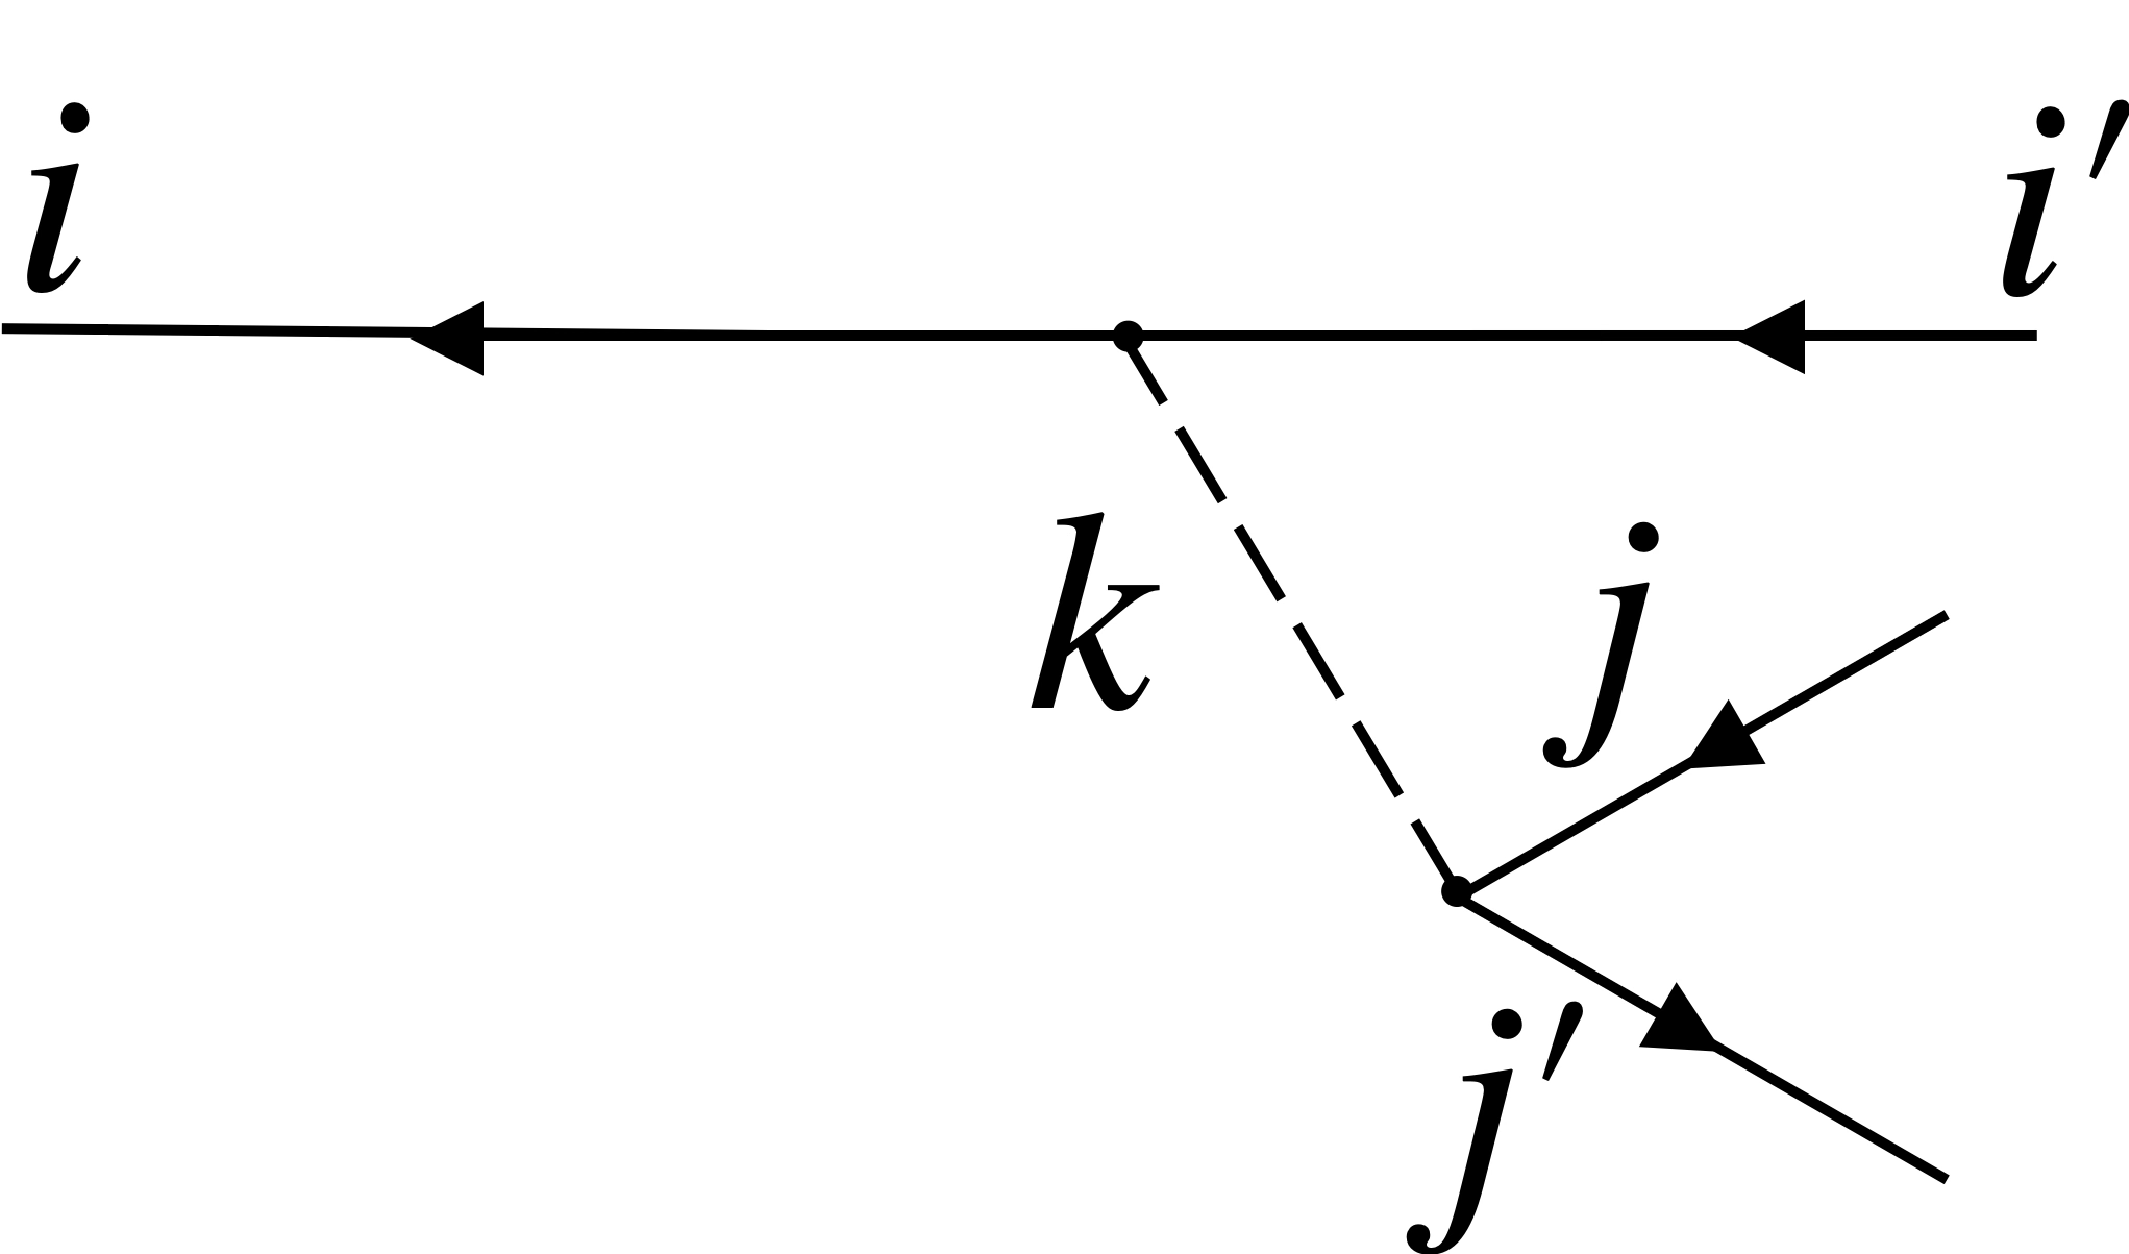
\includegraphics[width=0.15\textwidth]{figures/fffbar-f.pdf} & 
        {\small $\displaystyle 
        \int_{ijki'k'} \frac{(c_{i} - c_{j} - c_{j'} - c_{i'} - 2c_k)   c_{iki'}(0)  \tilde c^*_{ij'k}(0)}
        { (c_i - c_k - c_{i'})^2 + (c_k - c_{j'} - c_j)^2 -(c_i - c_j - c_{j'} - c_{i'})^2}
        \left( e^{-(c_i - c_j - c_{j'} - c_{i'})^2t} 
        - e^{-\left((c_i - c_k - c_{i'})^2 + (c_k - c_{j'} - c_j)^2\right)t} \right)
        b_i^\dagger b_{i'}   b_j d_{j'}
        $} \\
        \hline
        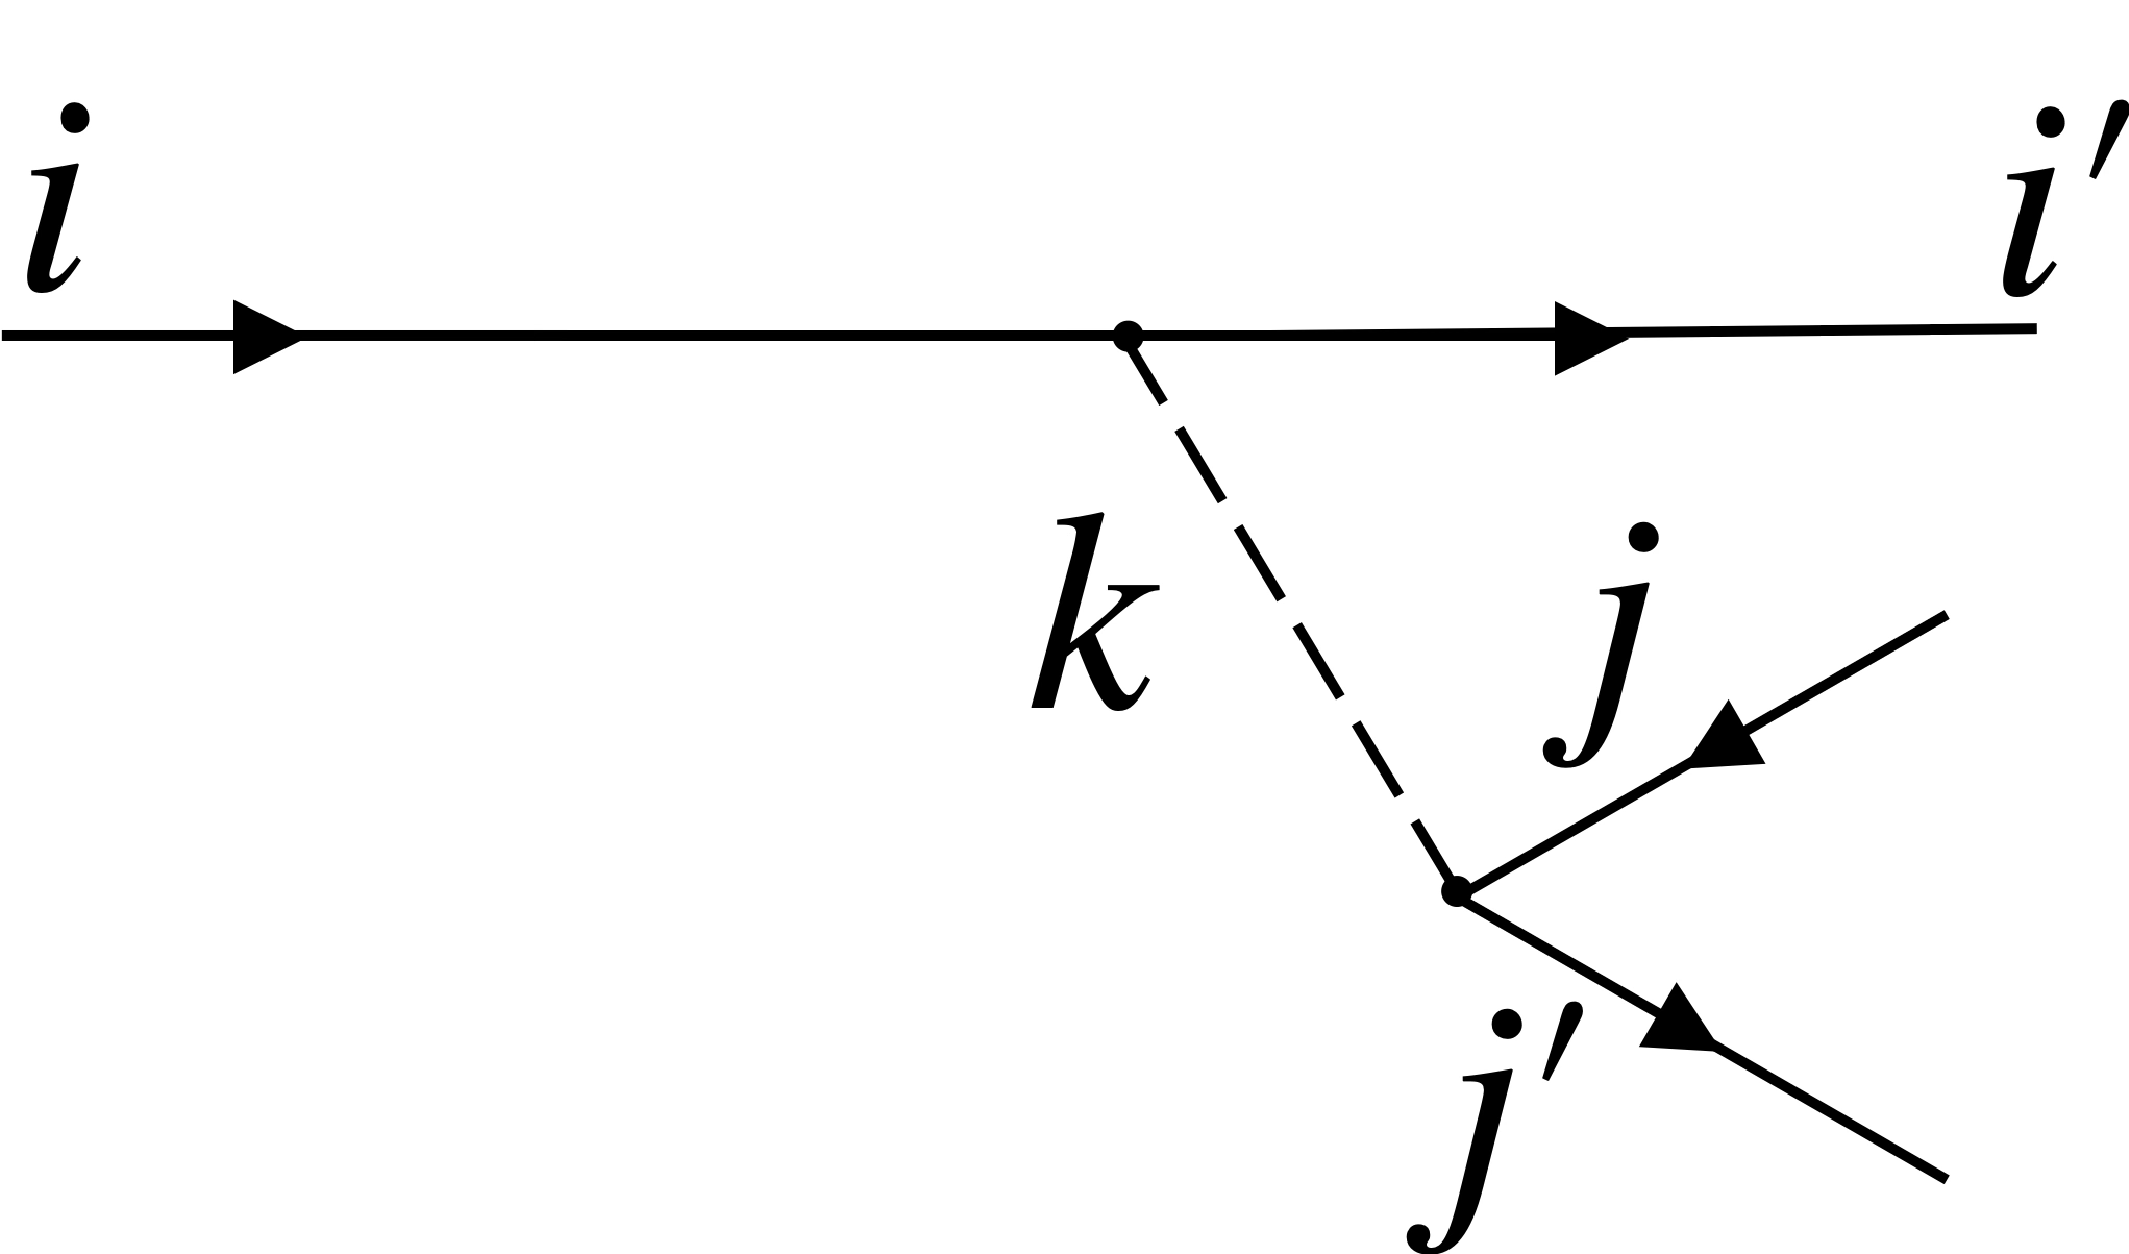
\includegraphics[width=0.15\textwidth]{figures/fbarfbarf-fbar.pdf} & 
        {\small $\displaystyle 
        \int_{ijki'k'} \frac{(c_{i} - c_{j} - c_{j'} - c_{i'} - 2c_k)   \bar c_{iki'}(0)  \tilde c^*_{ij'k}(0)}
        { (c_i - c_k - c_{i'})^2 + (c_k - c_{j'} - c_j)^2 -(c_i - c_j - c_{j'} - c_{i'})^2}
        \left( e^{-(c_i - c_j - c_{j'} - c_{i'})^2t} 
        - e^{-\left((c_i - c_k - c_{i'})^2 + (c_k - c_{j'} - c_j)^2\right)t} \right)
        b_j d_i^\dagger d_{i'}    d_{j'}
        $} \\
        \hline
        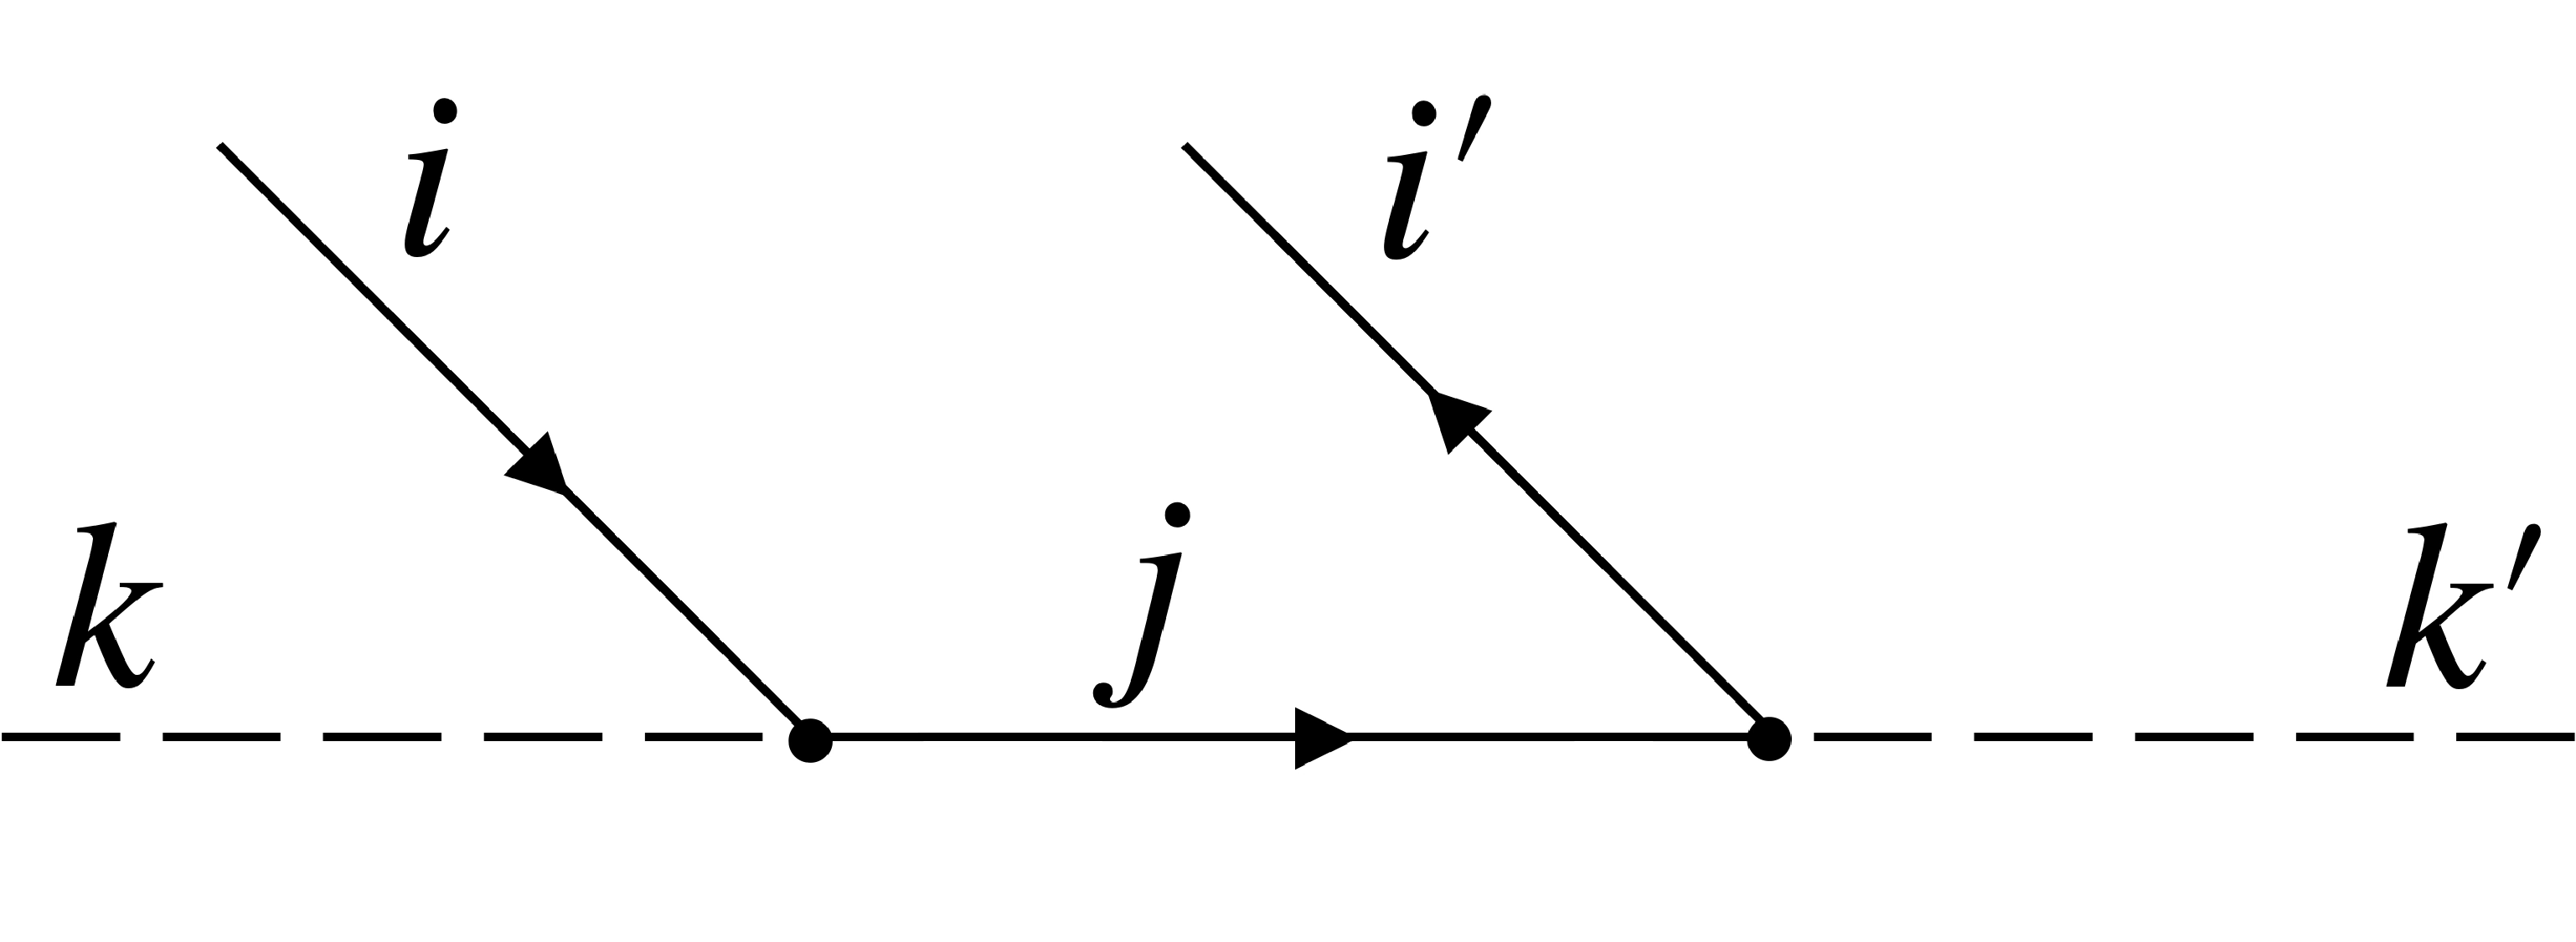
\includegraphics[width=0.15\textwidth]{figures/b-bffbar.pdf} & 
        {\small $\displaystyle 
        \int_{ijki'k'} \frac{(c_{k'} - c_{i'} - c_{i} - c_{k} - 2c_j) \bar c^*_{ikj}(0)  \tilde c_{i'jk'}(0)}
        { (c_i + c_k - c_j)^2 + (c_{i'} + c_j - c_{k'})^2 -(c_i + c_{i'} + c_k - c_{k'})^2}
        \left( e^{-(c_i + c_{i'} + c_k - c_{k'})^2t} 
        - e^{-\left((c_i + c_k - c_j)^2 + (c_{i'} + c_j - c_{k'})^2\right)t} \right)
        b_{i'}^\dagger d_i^\dagger a_k^\dagger a_{k'}
        $} \\
        \hline
        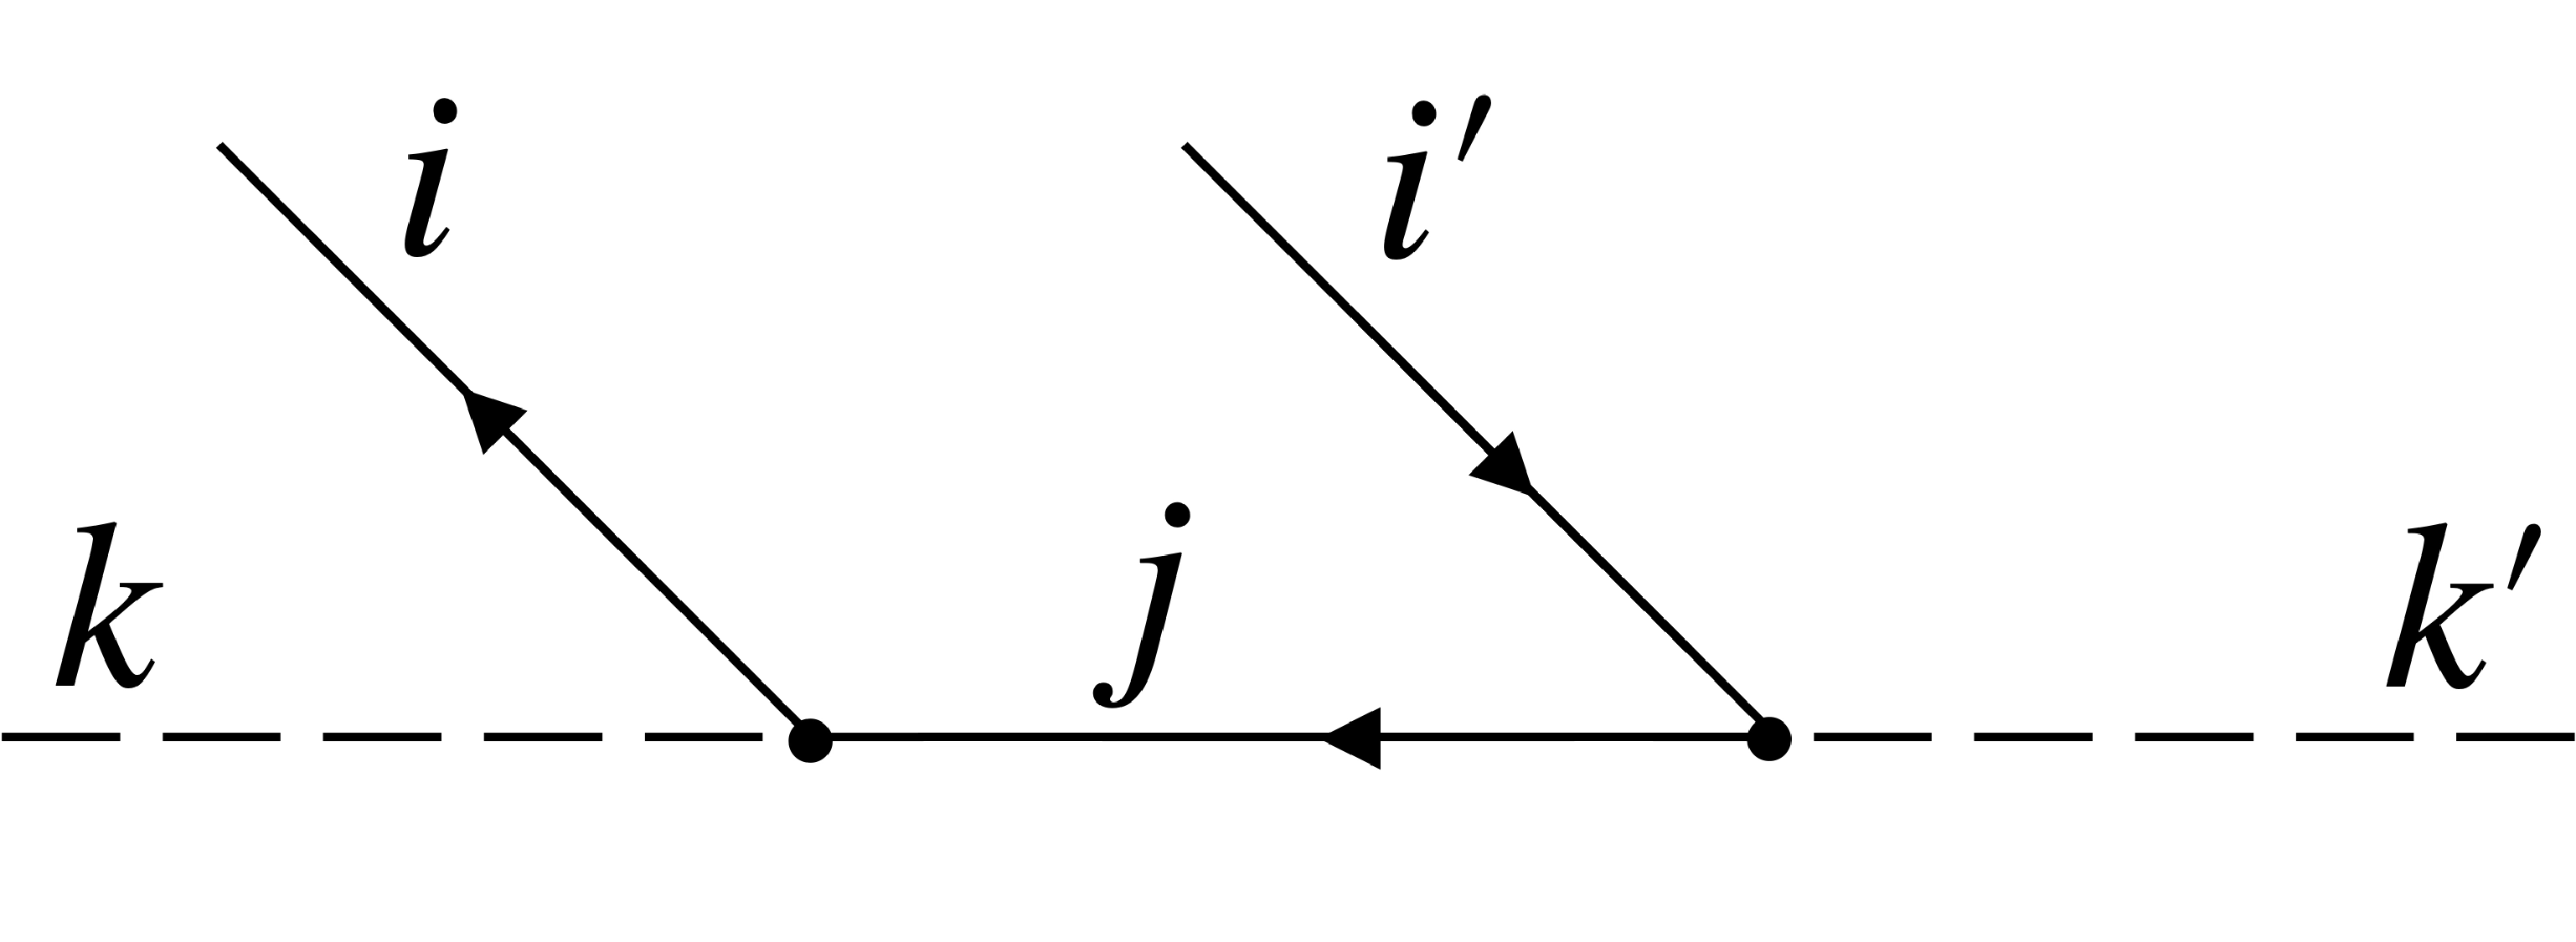
\includegraphics[width=0.15\textwidth]{figures/b-bffbar(2).pdf} & 
        {\small $\displaystyle 
        \int_{ijki'k'} \frac{(c_{k'} - c_{i'} - c_{i} - c_{k} - 2c_j)  c^*_{ji'k'}(0)  \tilde c_{kij}(0)}
        { (c_k - c_i - c_j)^2 + (c_j + c_{i'} - c_{k'})^2 -(c_k - c_i - c_{i'} - c_k)^2}
        \left( e^{-(c_k - c_i - c_{i'} - c_k)^2t} 
        - e^{-\left((c_k - c_i - c_j)^2 + (c_j + c_{i'} - c_{k'})^2\right)t} \right)
        b_{i}^\dagger d_{i'}^\dagger a_k^\dagger a_{k'} 
        $} \\
        \hline
        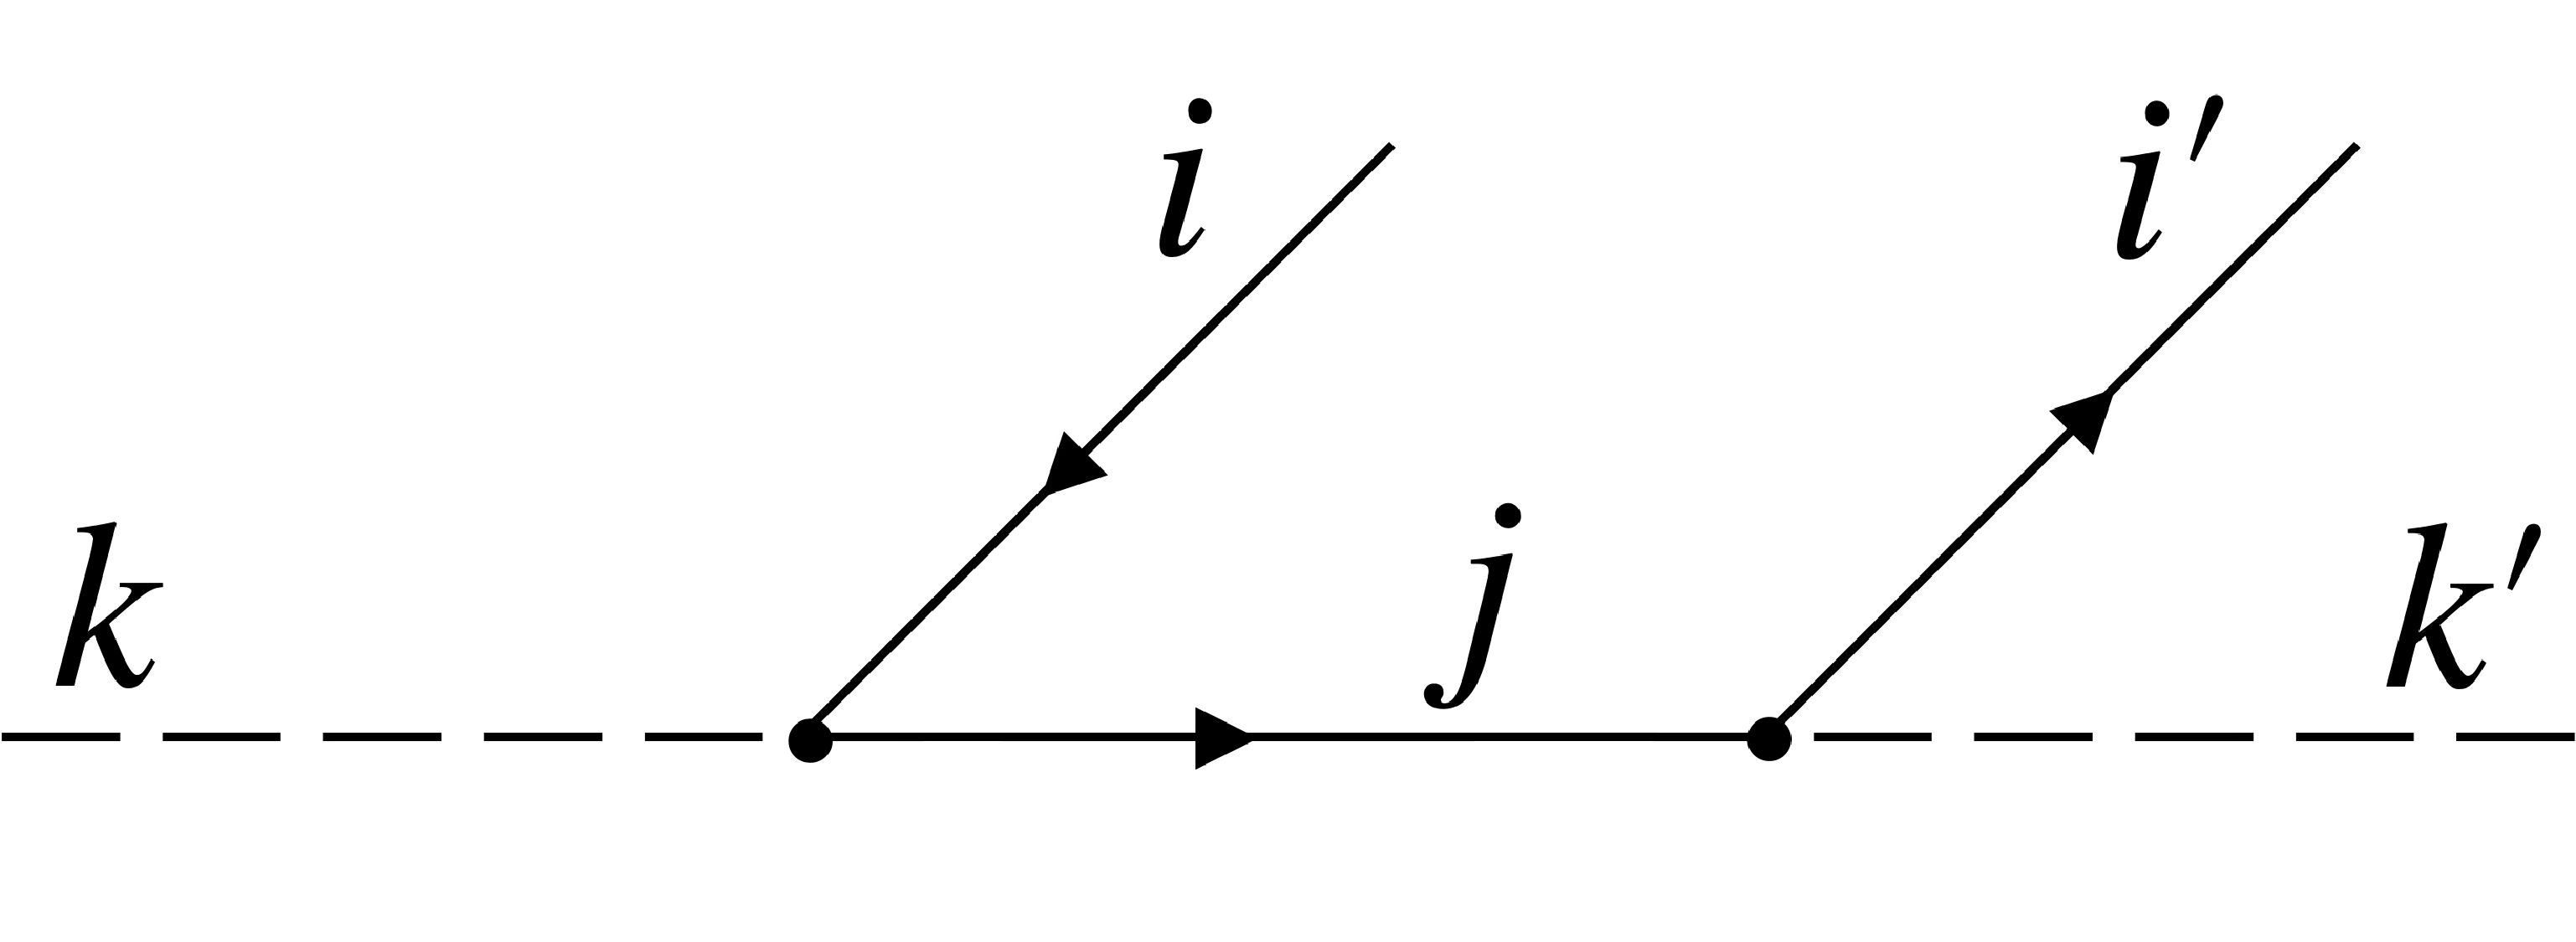
\includegraphics[width=0.15\textwidth]{figures/bffbar-b.pdf} & 
        {\small $\displaystyle 
        \int_{ijki'k'} \frac{(c_{k} - c_{i'} - c_{i} - c_{k'} - 2c_j) \bar c_{ikj}(0)  \tilde c^*_{i'jk'}(0)}
        { (c_i + c_k - c_j)^2 + (c_{i'} + c_j - c_{k'})^2 -(c_i + c_{i'} + c_k - c_{k'})^2}
        \left( e^{-(c_i + c_{i'} + c_k - c_{k'})^2t} 
        - e^{-\left((c_i + c_k - c_j)^2 + (c_{i'} + c_j - c_{k'})^2\right)t} \right)
        b_i d_{i'} a_{k}^\dagger a_{k'}
        $} \\
        \hline
        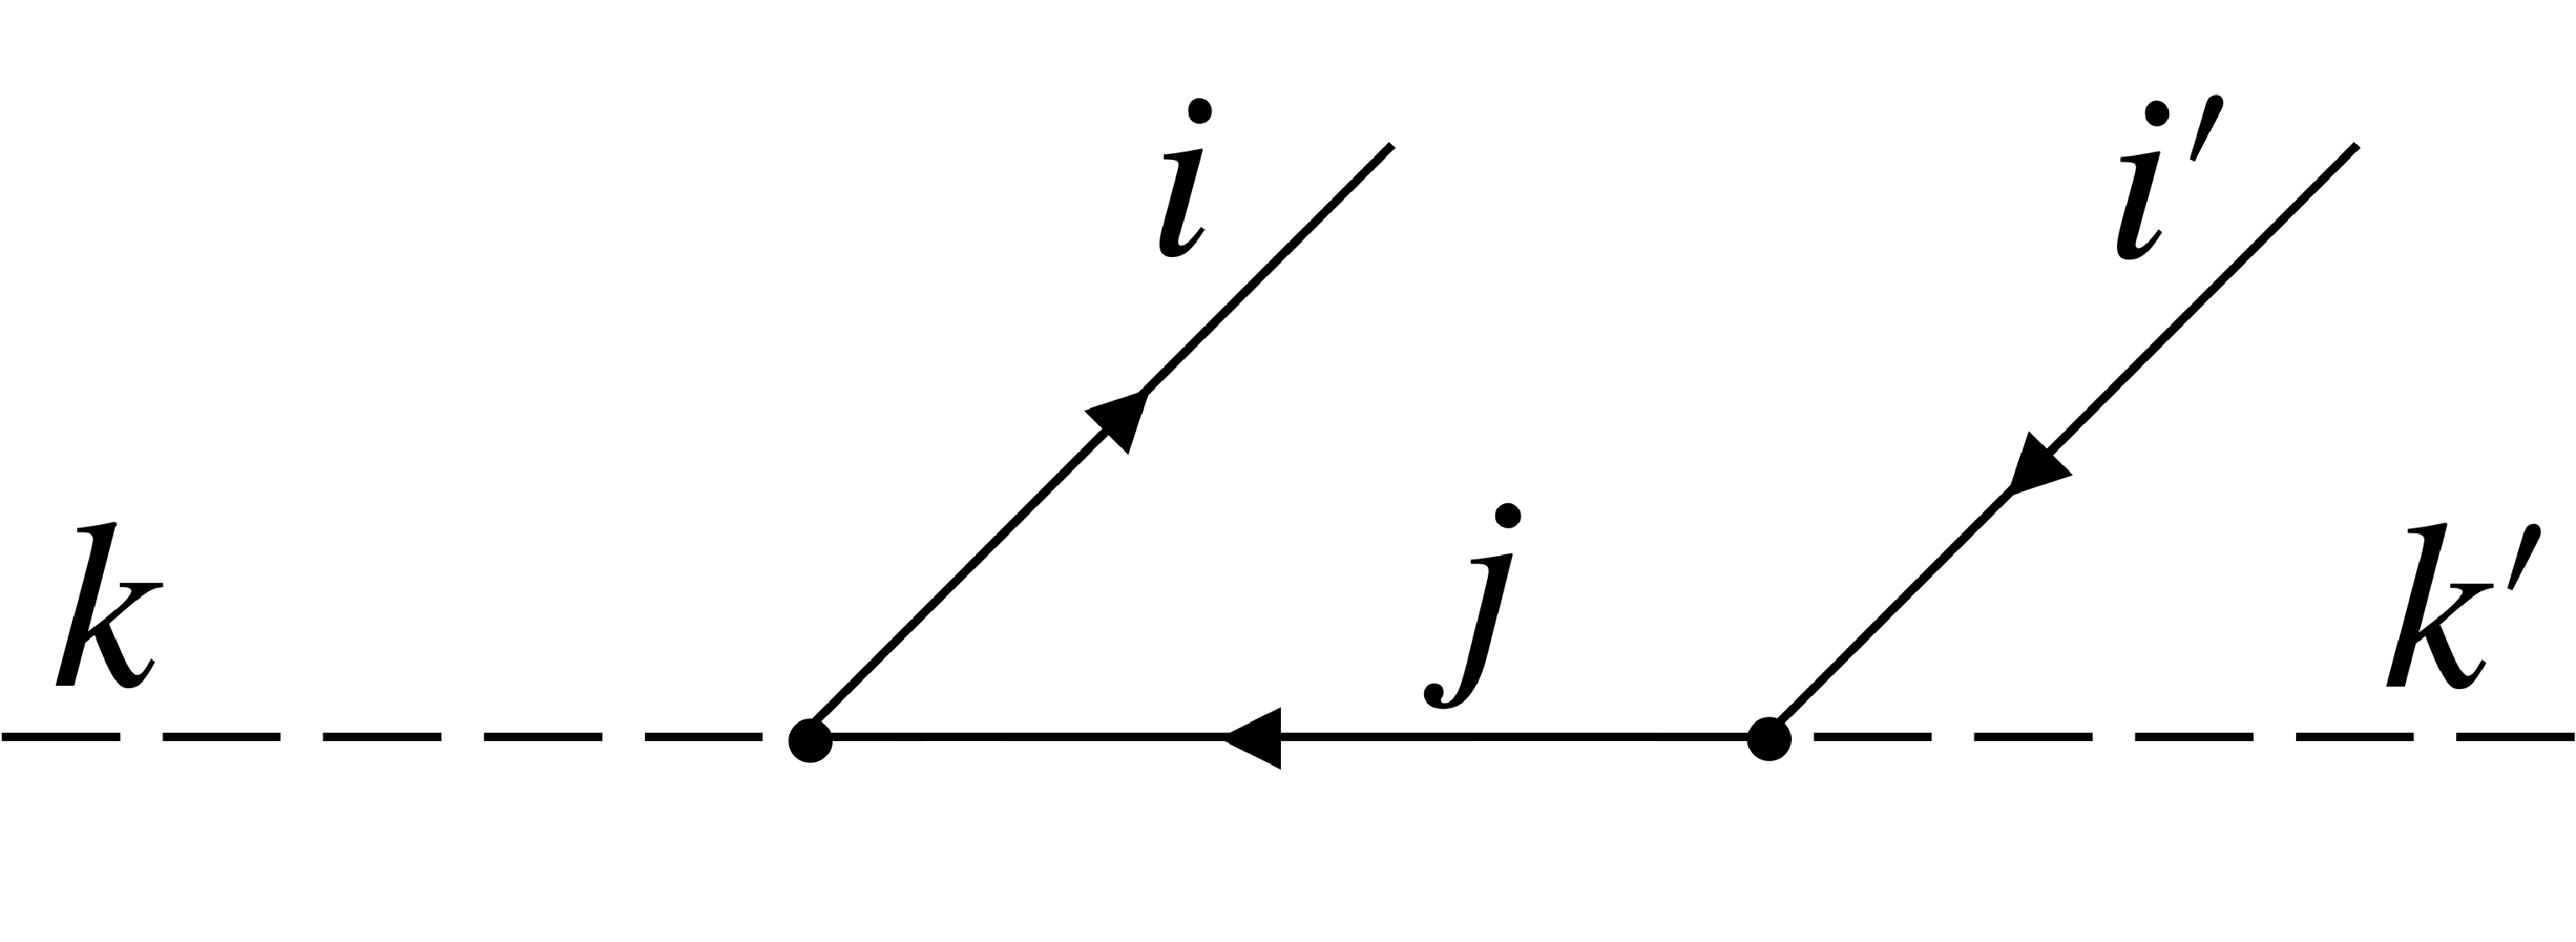
\includegraphics[width=0.15\textwidth]{figures/bffbar-b(2).pdf} & 
        {\small $\displaystyle 
        \int_{ijki'k'} \frac{(c_{k} - c_{i'} - c_{i} - c_{k'} - 2c_j) \tilde c^*_{kij}(0)  c_{ji'k'}(0)}
        { (c_i + c_k - c_j)^2 + (c_{i'} + c_j - c_{k'})^2 -(c_i + c_{i'} + c_k - c_{k'})^2}
        \left( e^{-(c_i + c_{i'} + c_k - c_{k'})^2t} 
        - e^{-\left((c_i + c_k - c_j)^2 + (c_{i'} + c_j - c_{k'})^2\right)t} \right)
        b_{i'} d_{i} a_{k}^\dagger a_{k'} 
        $} \\
        \hline
        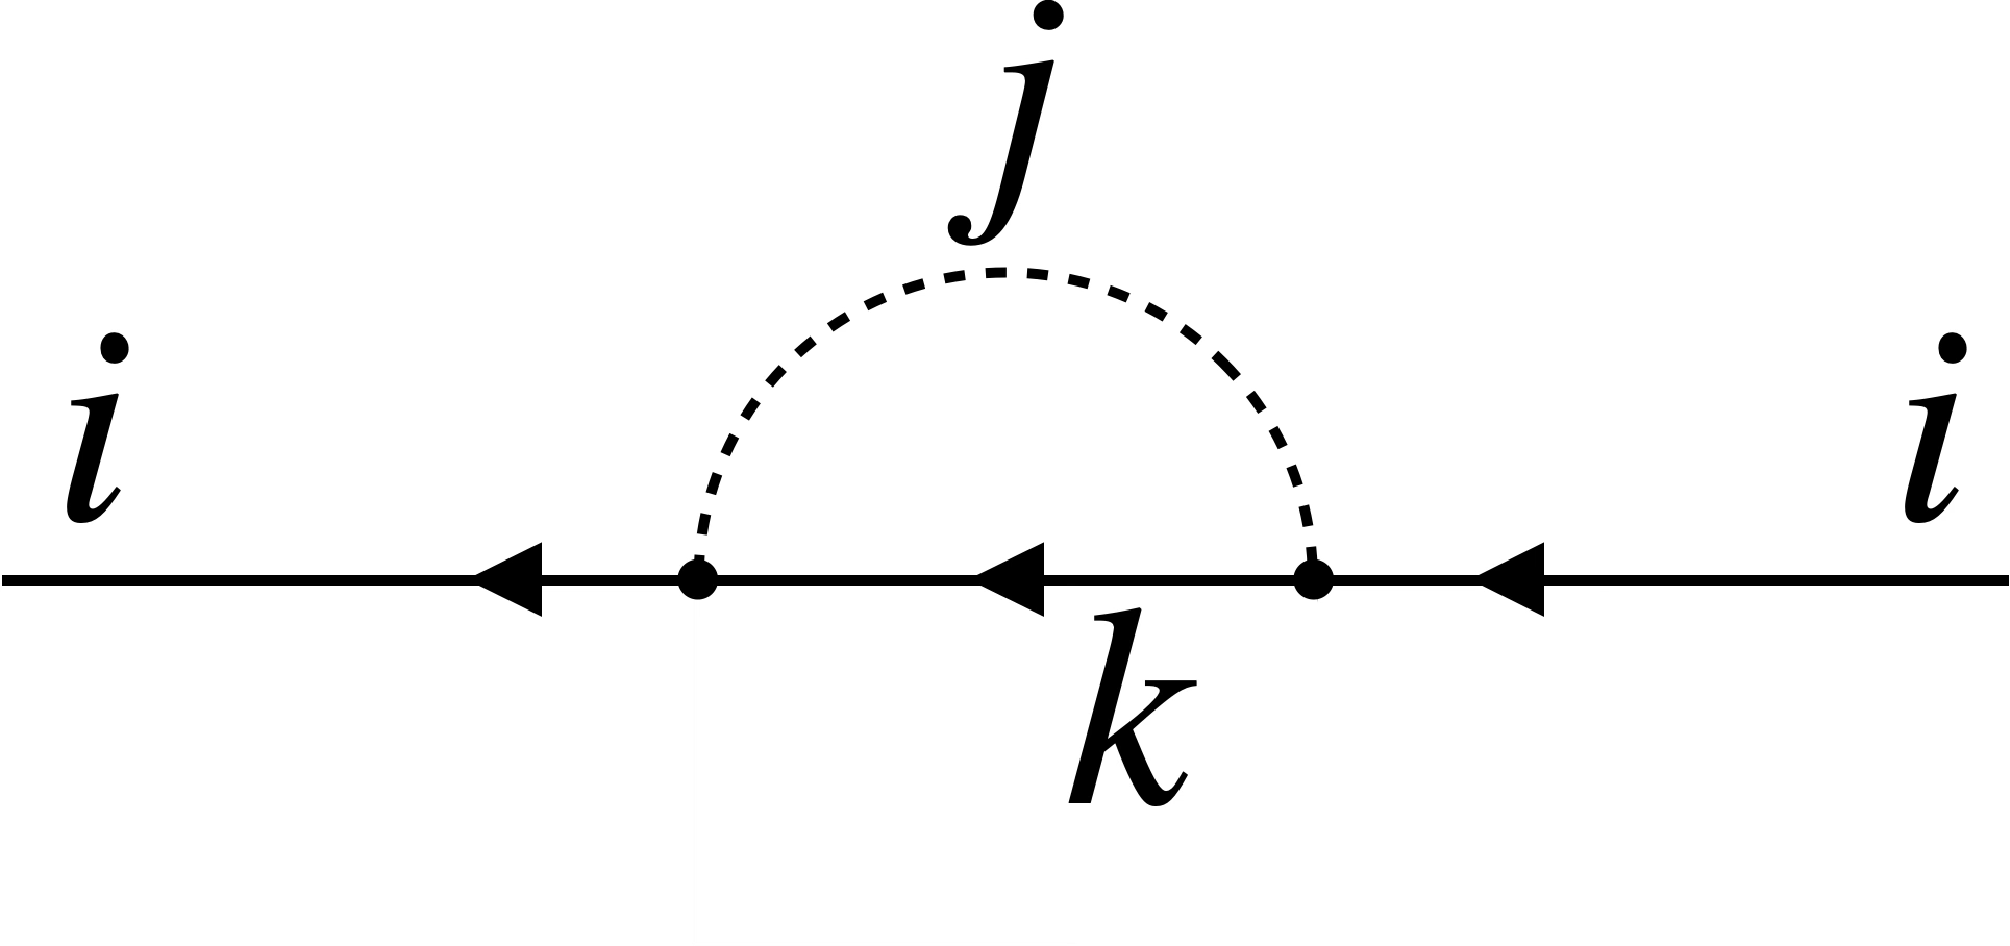
\includegraphics[width=0.15\textwidth]{figures/f-loop.pdf} & 
        {\small $\displaystyle 
        \int_{ijk} \frac{|c_{ijk}(0)|^2}{c_i - c_j - c_k}\left(1 - e^{-2\left(c_i - c_j - c_k \right)^2t} \right) b_i^\dagger b_i + \chi_{\delta_{m_F}}
        $} \\
        \hline
        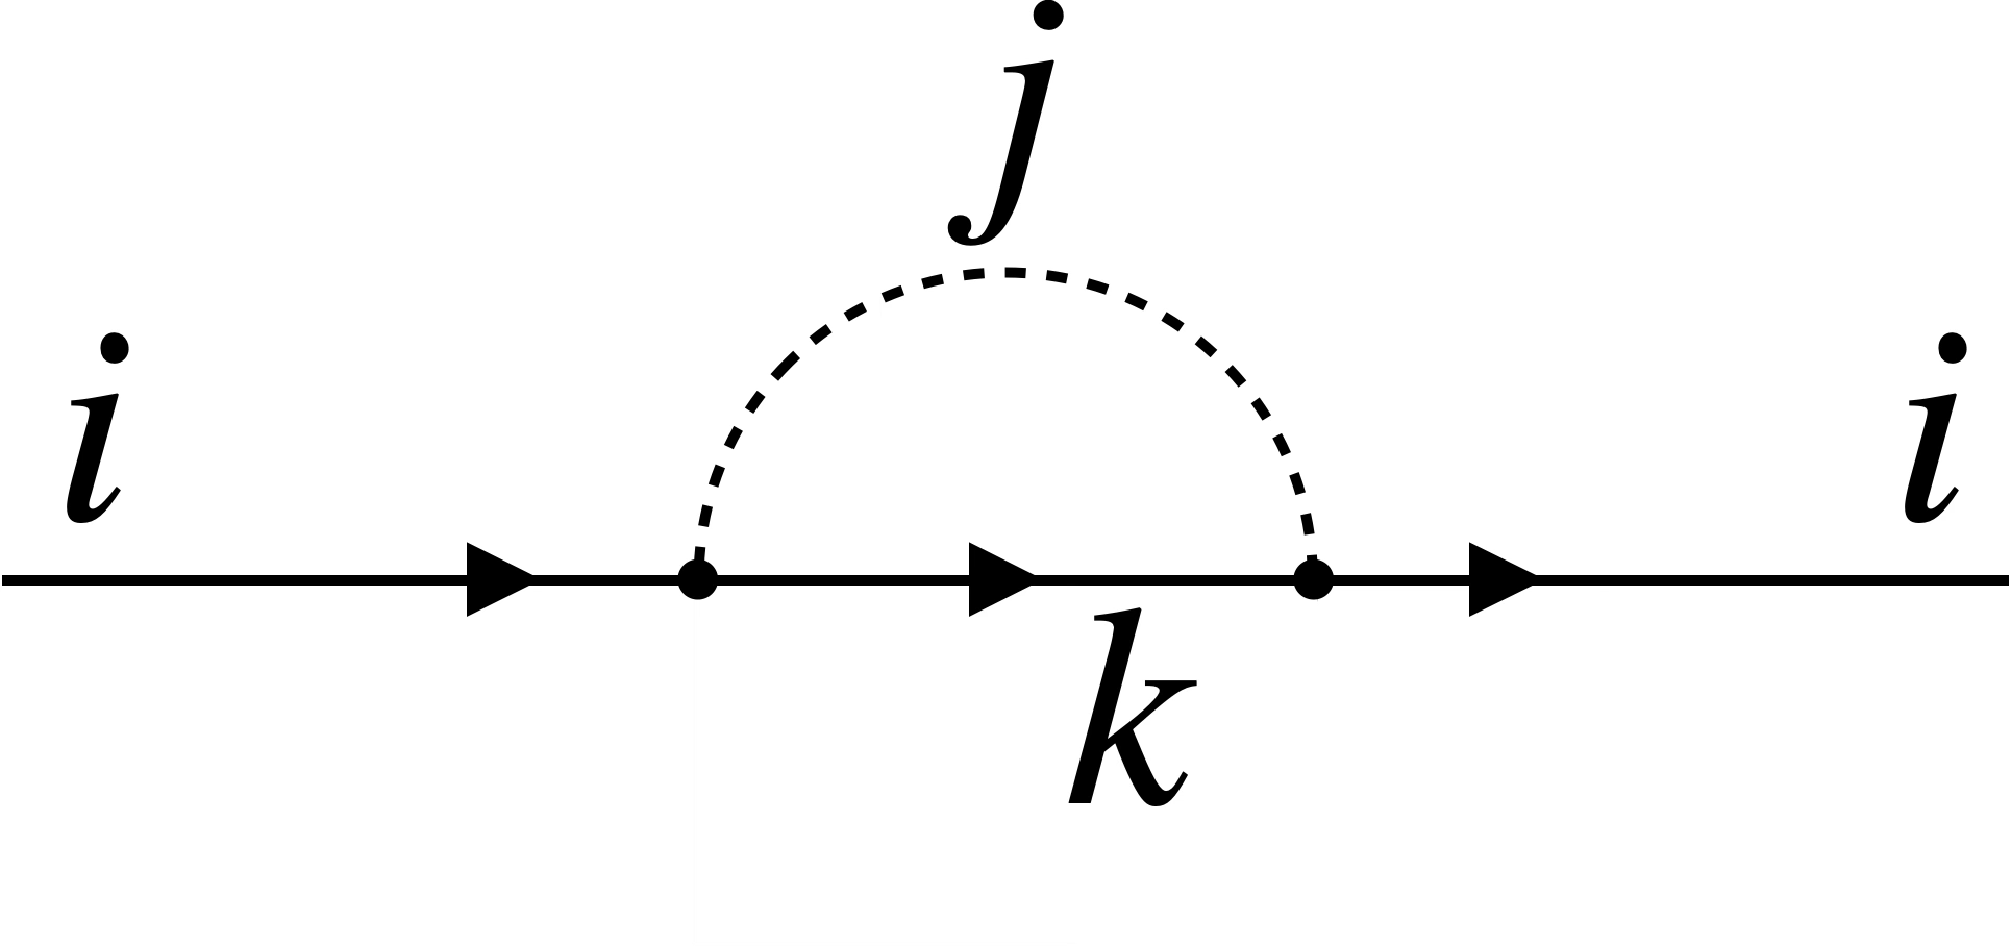
\includegraphics[width=0.15\textwidth]{figures/fbar-loop.pdf} & 
        {\small $\displaystyle 
        \int_{ijk} \frac{|\bar c_{ijk}(0)|^2}{c_i - c_j - c_k}\left(1 - e^{-2\left(c_i - c_j - c_k \right)^2t} \right) d_i^\dagger d_i + \chi_{\delta_{m_{\bar F}}}
        $} \\
        \hline
        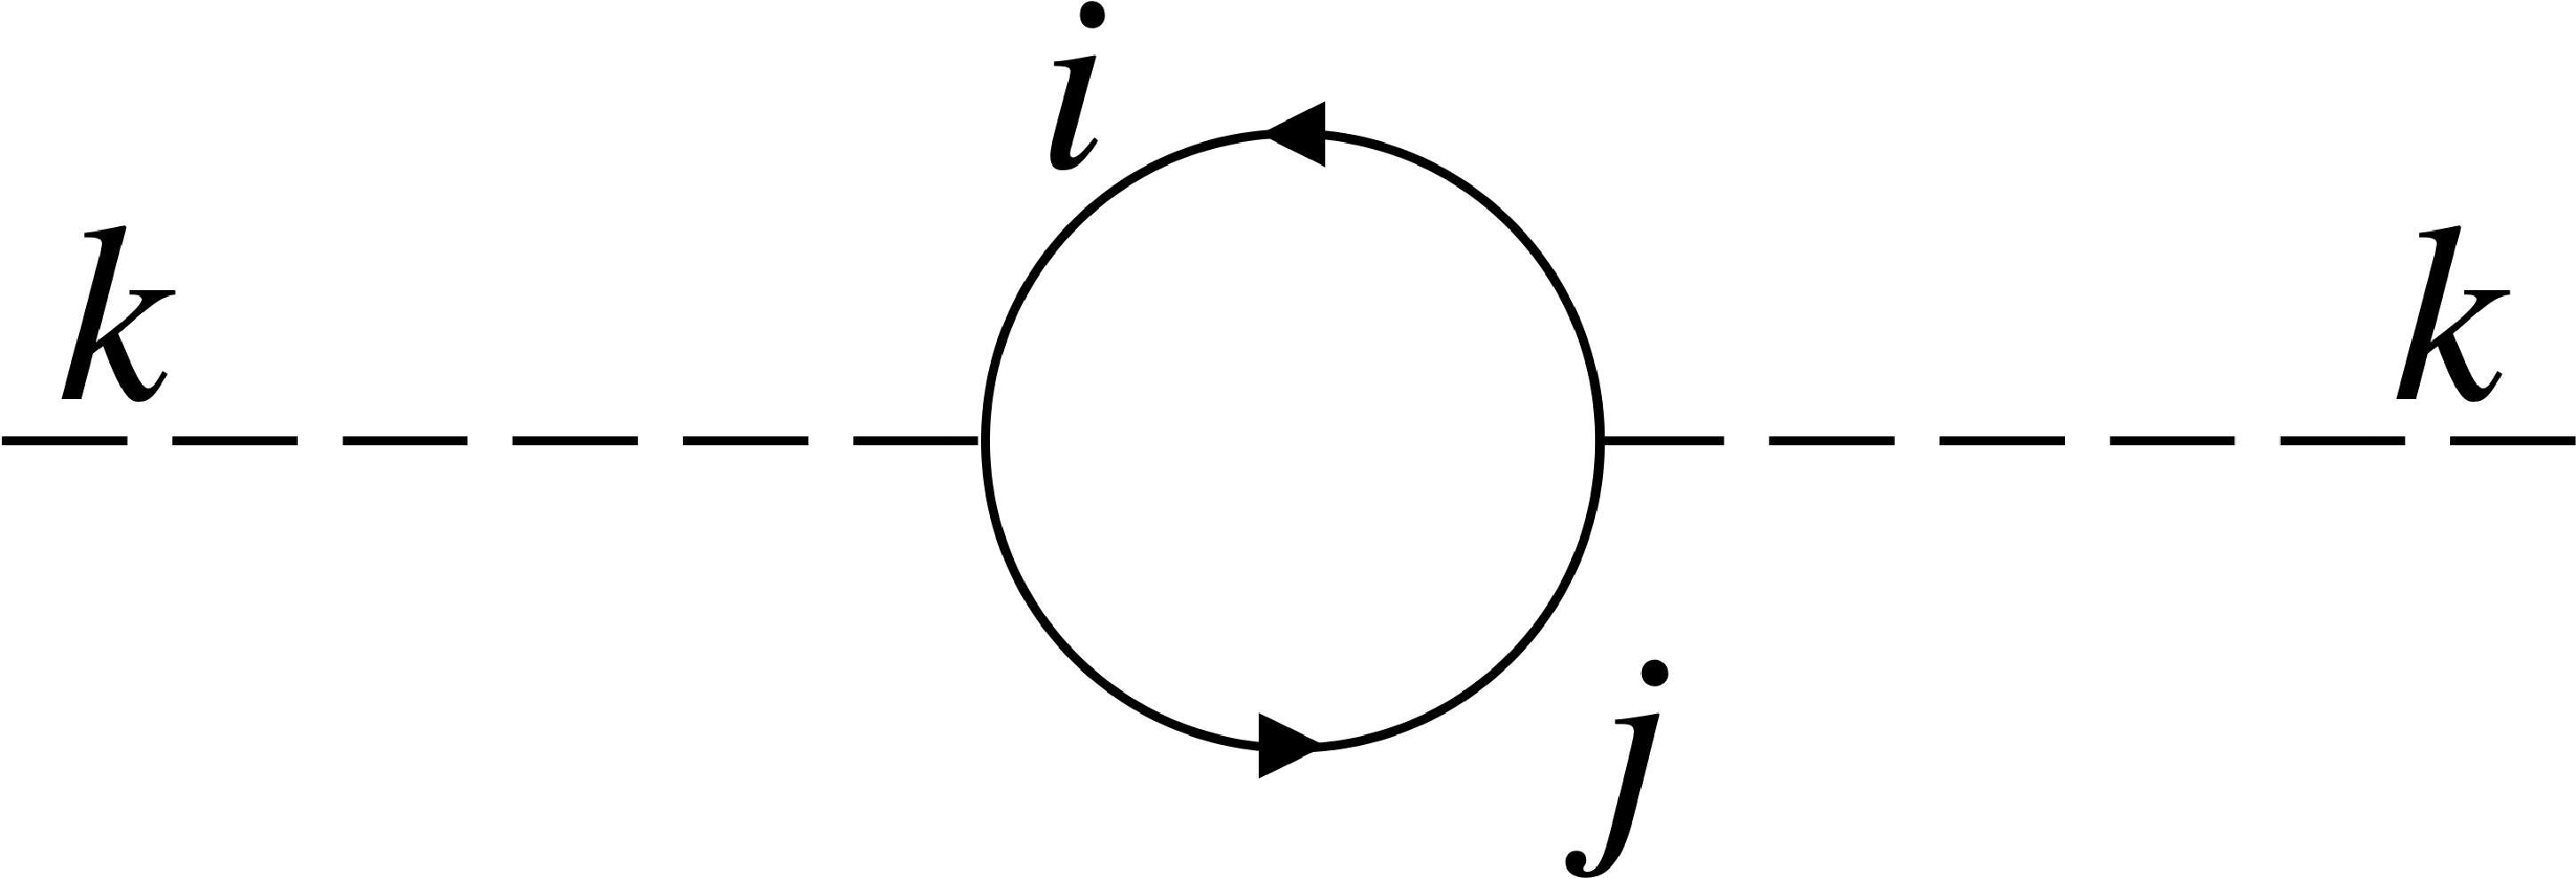
\includegraphics[width=0.15\textwidth]{figures/b-loop.pdf} & 
        {\small $\displaystyle 
        \int_{ijk} \frac{|\tilde c_{kij}(0)|^2}{c_k - c_i - c_j}\left(1 - e^{-2\left(c_k - c_i - c_j\right)^2t} \right) a_k^\dagger a_k + \chi_{\delta_{m_B}}
        $} \\
        \hline

    \end{tabular}
\end{table}

\begin{table}[h]
    \centering
    \hspace*{-1.7cm} % Move table to the left
    \begin{tabular}{|c|c|}
        \hline
        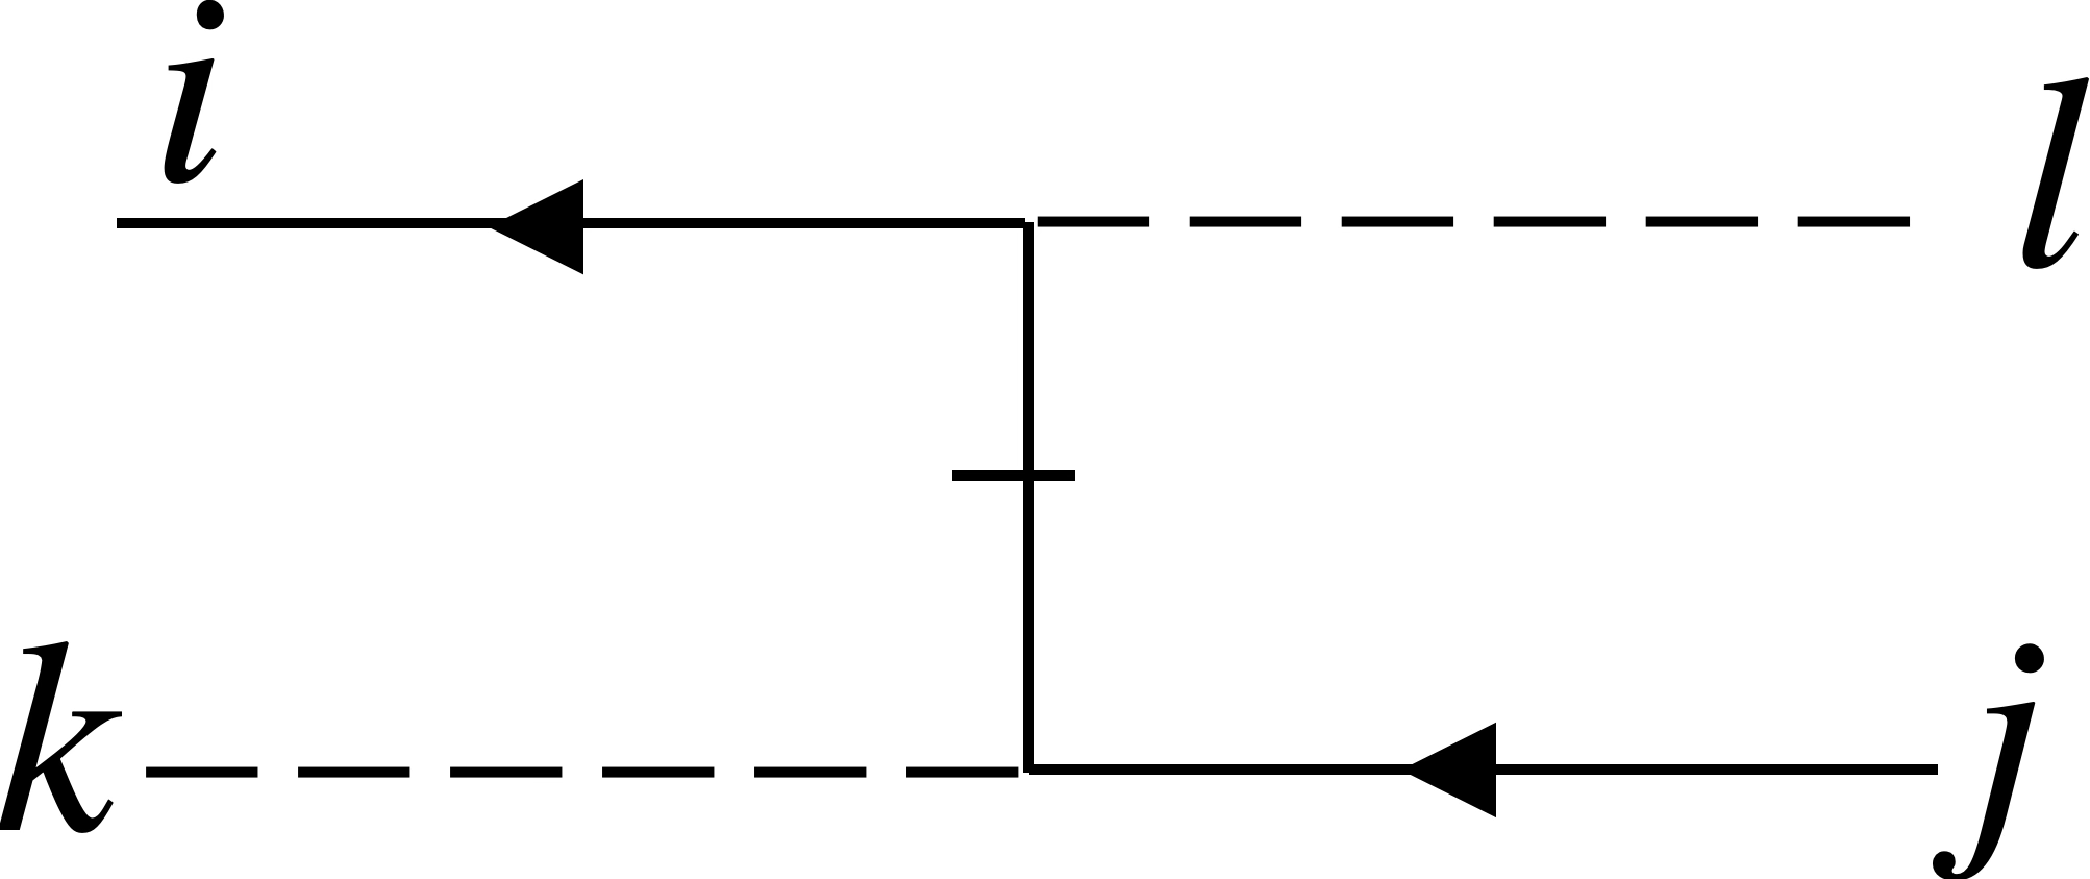
\includegraphics[width=0.15\textwidth]{figures/f-inst.pdf} & 
        {\small $\displaystyle 
        \int_{ijkl} \hat c_{ijkl}(0) e^{-\left(c_i + c_k - c_j - c_l \right)^2t} b_i^\dagger b_j a_k^\dagger a_l
        $} \\
        \hline
        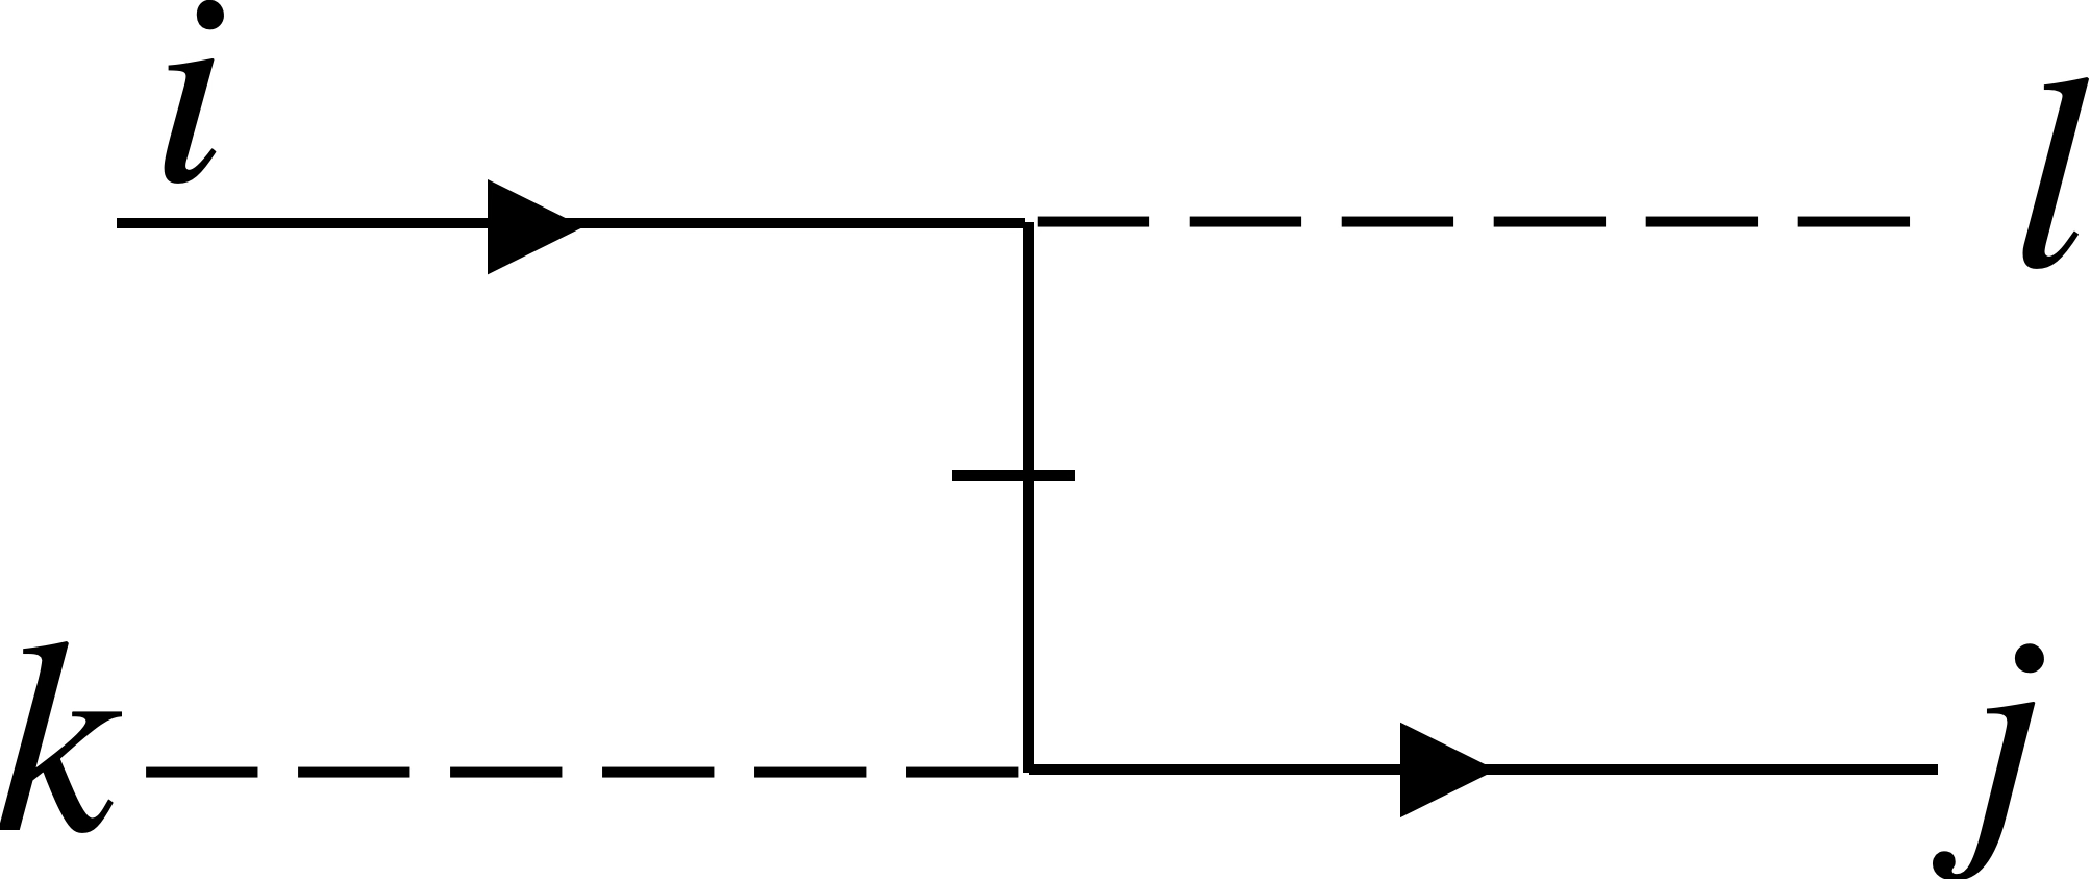
\includegraphics[width=0.15\textwidth]{figures/fbar-inst.pdf} & 
        {\small $\displaystyle 
        \int_{ijkl} \hat{\bar{c}}_{ijkl}(0) e^{-\left(c_i + c_k - c_j - c_l \right)^2t} d_i^\dagger d_j a_k^\dagger a_l
        $} \\
        \hline

    \end{tabular}
    \caption{Terms that make up $H^{(2)}(t)$} 
    \label{tab:H2}

\end{table}